\pagestyle{empty}
\graphicspath{{Aplicaciones/}}
\part{Las aplicaciones  y usos pr�cticos}

\onecolumn

\sffamily

\vspace*{4cm}

En esta parte se presentan casos pr�cticos del uso de SIG en diversas disciplinas. De este modo, podr� comprobarse la versatilidad de este y ver c�mo todo aquello que hemos estudiado en las partes anteriores de este libro tiene una aplicaci�n real en campos muy variados. 

En cada cap�tulo se destacan los elementos particulares que resultan de mayor inter�s para el caso tratado, tomados de entre todos los que ya conocemos del �mbito SIG. Asimismo, se presentar�n algunos nuevos y m�s espec�ficos cuando ello resulte relevante. %Junto a esto, casos reales de aplicaci�n ayudan a completar el contenido de cada tema.

\begin{itemize}
\item El cap�tulo \ref{Introduccion_aplicaciones} presenta en l�neas generales el conjunto de disciplinas y grupos de inter�s que pueden beneficiarse del uso de SIG, al tiempo que explora la presencia de estos en distintos �mbitos.

\item El cap�tulo \ref{Analisis_riesgos} trata la aplicaci�n de los SIG a distintos an�lisis relacionados con riesgos naturales tales como inundaciones, incendios, movimientos de tierras, plagas o contaminaci�n de aguas.

\item El cap�tulo \ref{Ecologia} repasa las principales aplicaci�n del SIG dentro del campo de la ecolog�a tales como la modelizaci�n de comunidades animales o vegetales, entre otras.

\item Relacionado con el anterior, el cap�tulo \ref{Gestion_ambiental} trata el uso de SIG para la gesti�n de recursos naturales y la planificaci�n territorial.

%\item El cap�tulo \ref{Geomarketing} trata el uso de los SIG en el mundo de los negocios, describiendo particularmente su uso dentro de lo que se conoce como \emph{geomarketing}.

\end{itemize}

\rmfamily
%\twocolumn

\chapter{Introducci�n. �Para qu� puedo utilizar un SIG?}
\label{Introduccion_aplicaciones}
\pagestyle{fancy}



\bigskip

\begin{intro}
Los SIG son herramientas muy vers�tiles y no existe pr�cticamente ning�n �mbito de trabajo en el que los SIG no puedan, de un modo u otro, ser de utilidad. En este cap�tulo, veremos c�mo la flexibilidad de los SIG les ha permitido incorporarse en las tareas de las m�s diversas disciplinas y veremos estas de modo gen�rico. En los siguientes cap�tulos, trataremos en profundidad las particularidades del uso de SIG en las principales disciplinas, y el objeto de este cap�tulo es presentar de forma gen�rica todo ese conjunto de �mbitos beneficiarios del SIG y describir sus caracter�sticas comunes, analizando qu� utilidades generales tiene un SIG dentro de todos ellos.
\end{intro}

\section{Introducci�n}

A lo largo de los anteriores cap�tulos, hemos visto qu� es un SIG, cu�les son sus componentes y sus caracter�sticas principales, y qu� tipo de tareas y procesos pueden llevarse a cabo con ellos. Todos estos elementos pueden ser aprovechados de formas muy distintas por los diferentes grupos de usuarios en funci�n de sus necesidades, ya que, por su propia naturaleza, un SIG es una herramienta altamente vers�til. Como sistema complejo, puede adaptarse a las circunstancias particulares de un gran n�mero de situaciones y entornos, los cuales tender�n a hacer uso prioritario de unas u otras capacidades de un SIG. 

En algunas disciplinas, el an�lisis es el elemento fundamental, y los SIG en ellas se entienden principalmente como herramientas anal�ticas. En otras, sin embargo, las capacidades de visualizaci�n y representaci�n pueden resultar mucho m�s importantes, aprovech�ndose estas de forma preferente y utilizando las capacidades de an�lisis en menor medida.

En conjunto, todas estas capacidades (an�lisis, visualizaci�n, manejo de datos, etc.) que ya hemos visto con detalle en las partes anteriores del libro ofrecen una serie de utilidades que son las que cada comunidad de usuarios emplea de modo particular seg�n sea las necesidades de su trabajo.

En este cap�tulo detallaremos esas utilidades y veremos qu� elementos de un SIG est�n implicados en ellas. Posteriormente, recorreremos el amplio abanico de campos de aplicaci�n de los SIG, perfilando las funciones b�sicas de un SIG que resultan de mayor inter�s en ellos. Como es l�gico pensar, resulta imposible describir todos los posibles casos de aplicaci�n de los SIG, siendo estos excesivamente numerosos. Centraremos el contenido de este cap�tulo en tratar los principales grupos de disciplinas afines, describiendo brevemente el papel que los SIG juegan en ellas.

Las m�s representativas de estas disciplinas ser�n tratadas con m�s detalles en los restantes cap�tulos de esta parte del libro, describiendo no solo la utilidad de los SIG sino las formulaciones concretas que se utilizan en cada caso, las soluciones particulares en cada uno de estos campos en t�rminos de tecnolog�a SIG, as� como otros elementos particulares de cada �mbito de aplicaci�n.

\section{Caracterizaci�n de las aplicaciones de un SIG}

Los SIG son herramientas �tiles desde muchos puntos de vista, y act�an como herramientas vers�tiles de las que puede sacarse uno u otro provecho seg�n el enfoque adoptado. Para clasificar los diferentes �mbitos de aplicaci�n de los SIG no solo debe atenderse al �mbito en s�, sino tambi�n a la funcionalidad que del SIG se espera en cada uno de ellos, y de algunos otros aspectos relativos a los distintos elementos que conforman el SIG. De esta forma se pueden definir los grupos comunes de actividad existentes en torno al SIG y los elementos que las agrupan o diferencian.

Entre los factores que pueden emplearse para esta clasificaci�n, podemos citar algunos como los siguientes.

\begin{itemize}
\item Procesos principales de inter�s.
\item Tipo fundamental de datos con los que se trabaja.
\item Volumen de variables y datos empleados.
\item Precisi�n de trabajo necesaria.
\item Tipo de usuarios de SIG esperados.
\item Complejidad de las operaciones y tareas desarrolladas.
\item Medida en que los SIG responden a las necesidades existentes.
\end{itemize}

Aunque una clasificaci�n en funci�n de estos criterios puede resultar notablemente difusa (no olvidemos que el SIG es una herramienta integradora y las posibilidades ser�an muy numerosas y con gran variabilidad), estas circunstancias resultan de inter�s para estudiar c�mo es la presencia de los SIG en cada uno de los campos de aplicaci�n principales.

Es importante asimismo clasificar el papel que el SIG desempe�a dentro del trabajo que habitualmente se lleva a cabo en cada disciplina, para de este modo poder entender mejor su importancia y extraer de su aplicaci�n la mayor funcionalidad posible. Desde el punto de vista del usuario es de inter�s conocer <<qu� se puede hacer con un SIG>> pero tambi�n <<por qu� podemos hacer eso con un SIG>>, ya que de este modo se tiene un conocimiento m�s rico de los SIG como herramientas. Conocer lo que otros usuarios hacen con un SIG enriquece nuestro propio conocimiento de este.

Algunos de los papeles principales que un SIG puede jugar son los siguientes.

\begin{itemize}

\item SIG como herramienta modelizadora. Utilizando los diferentes procesos de an�lisis espacial implementados en un SIG, pueden modelizarse realidades geogr�ficas complejas. Como ya vimos en el cap�tulo \ref{SIGs_escritorio}, la combinaci�n de an�lisis sencillos mediante la definici�n de flujos de trabajo permite generar operaciones de mayor complejidad que contengan modelos de diversa �ndole. Las funcionalidades de los SIG en este sentido los hacen igualmente adecuados para modelos tanto de tipo conceptual como matem�tico, y ya sean estos est�ticos o din�micos.

Procesos de todo tipo pueden ser modelizados de este modo, y permiten no solo obtener resultados directos, sino tambi�n contribuir a una mejor comprensi�n del proceso en s� y de los mecanismos que lo rigen, lo cual amplia notablemente la utilidad de los SIG como herramientas modelizadoras.

\item SIG como herramienta para la toma de decisiones. Gran parte de los campos en los que se puede aplicar un SIG requieren en alg�n momento tomar decisiones en funci�n de ciertas variables. Estas variables implican dentro de un SIG el uso de distintas capas, normalmente en n�mero elevado. La combinaci�n de estas arroja resultados que resultan m�s adecuados para su interpretaci�n por parte de un t�cnico experto, que ser� el encargado de tomar las decisiones. 

Las t�cnicas de evaluaci�n multicriterio que ya conocemos se aplican en gran n�mero de disciplinas, y el SIG resulta la herramienta perfecta para aplicarlas. La cantidad elevada de variables (capas) que se manejan en estos procesos hace necesaria una herramienta que facilite el uso conjunto de todas ellas, al mismo tiempo que permita una visi�n global del conjunto de datos que se manejan, y el SIG cumple todos los requisitos para ser dicha herramienta. 

La toma de decisiones representa una utilizaci�n particular de las capacidades de modelizaci�n citadas anteriormente, en la que la interpretaci�n de los resultados es el elemento clave, apoyada fuertemente en las capacidades anal�ticas del SIG. 

\item SIG como herramienta para la difusi�n de informaci�n geogr�fica. Su capacidad para exponer los datos geogr�ficos a un p�blico m�s amplio y hacerlo de una forma �ptima es una de las virtudes m�s notables de los SIG, especialmente con las tecnolog�as actuales y la situaci�n existente hoy en d�a. Para muchas disciplinas, poder hacer llegar la informaci�n geogr�fica a ciertos destinatarios supone un hecho importante, y es por ello que los SIG resultan herramientas �tiles en esos casos.

No se ha de olvidar que los SIG, como ya dijimos, ponen de manifiesto la naturaleza espacial de muchos datos, y por ello son un veh�culo perfecto para la difusi�n de todo tipo de informaci�n geogr�fica. En otras palabras, el SIG es una herramienta muy potente para ampliar el alcance de la informaci�n geogr�fica, y que todos aquellos que puedan sacar partido de ella tengan a su disposici�n esa informaci�n sin dificultad alguna.

Esto es de importancia en muchos campos no t�cnicos, jugando las tecnolog�as Web un papel clave para hacer llegar a usuarios sin perfil t�cnico datos y elementos SIG que dan valor a la informaci�n con que estos trabajan. Informaci�n que antes se mostraba sin componente geogr�fica alguna ahora puede acompa�arse de forma sencilla de mapas interactivos u otros elementos SIG, a la vez que se ofrece a los usuarios una serie de funcionalidades propias de los SIG, a trav�s de las cuales podr�n realizar un uso m�s intenso y completo de esa informaci�n. En los campos m�s t�cnicos, no obstante, tambi�n se benefician de este hecho, y la mayor disponibilidad de la informaci�n geogr�fica es responsable directa de avances o descubrimientos, pues act�a como un catalizador de estos (puede consultarse \cite{webBBCArqueologia} para un caso peculiar, aunque no aislado, de lo anterior).

\item SIG como herramienta centralizadora. Cuando el factor humano es el m�s importante para el desarrollo de una determinada actividad, la capacidad organizativa de un SIG como sistema apto para coordinar las tareas de un equipo de trabajo resulta determinante. Este hecho es especialmente relevante cuando se trabaja en el seno de una organizaci�n voluminosa en la cual pueden coexistir usuarios de informaci�n geogr�fica con distintos intereses. Tal es el caso de un SIG corporativo instalado en una gran empresa o en una administraci�n local, en la que las necesidades que se presentan cubren un abanico muy amplio.

En esta circunstancia el SIG act�a como un elemento central para facilitar el acceso de todas las personas implicadas a la informaci�n geogr�fica y garantizar que ese acceso se realiza de forma correcta. El SIG es ante todo una herramienta para la gesti�n de la informaci�n geogr�fica, y los principales (aunque no �nicos) beneficiarios de la tecnolog�a SIG son en este caso los responsables de esa informaci�n, quienes organizan y gestionan el gran volumen de datos del que se dispone. Estos tienen a su vez el papel m�s importante dentro de todos los profesionales implicados en el sistema SIG, pues el dise�o e implementaci�n de la base de datos geogr�fica correspondiente, as� como su mantenimiento, son vitales para el buen funcionamiento del SIG y que este pueda dar respuesta a todos los requerimientos existentes.

\end{itemize}

\section{�reas de aplicaci�n de un SIG}

Con los elementos vistos en el apartado anterior, podemos caracterizar en t�rminos generales la forma en que los distintos campos de aplicaci�n hacen uso de los SIG para su trabajo habitual. Algunas de las principales �reas de utilizaci�n de un SIG las siguientes:

\subsection{Gesti�n de recursos naturales}

La gesti�n de recursos naturales es uno de los campos que llevan aprovechando las tecnolog�as y elementos SIG desde su mismo origen. De hecho, y como ya vimos al inicio de este libro, las necesidades originadas en este �rea fueron responsables del desarrollo de los primeros SIG, y fueron estas necesidades las que originalmente definieron las capacidades y caracter�sticas de los SIG en sus inicios.

Por ello, los SIG son herramientas excepcionales para la gesti�n de la informaci�n sobre los distintos recursos naturales, y la explotaci�n de la gran cantidad de datos de los que se dispone en este campo. Estos datos pueden ser de tipos muy variados, y ello hace que tanto datos vectoriales como r�ster sean de gran importancia para este tipo de an�lisis.

La labor de gesti�n de datos de un SIG es importante en este campo, pero tambi�n lo es su capacidad de an�lisis, ya que las necesidades de tipo anal�tico que presenta la gesti�n de recursos naturales es elevada.

\subsection{Gesti�n de riesgos}

Los riesgos, tanto los naturales como los generados por las actividades humanas, pueden analizarse en un SIG, estudiando su distribuci�n o tratando de evaluar la probabilidad de que se produzcan episodios problem�ticos. Se trata, por tanto, de una labor fundamentalmente de an�lisis, y es este un campo en el que se emplean gran parte de las t�cnicas que hemos visto en la parte dedidada al an�lisis en este libro.

Los datos que se emplean son principalmente de tipo r�ster, ya que gran parte de las variables con las que se trabaja son de tipo continuo. No obstante, los registros de ocurrencia de fen�menos como incendios, avalanchas o inundaciones se recogen mejor en datos de tipo vectorial, y las metodolog�as en este campo combinan frecuentemente ambos tipos de datos.

Los usuarios de SIG en este terreno son de tipo avanzado y exigen de los SIG una amplia serie de funcionalidades, en ocasiones requiriendo gran n�mero de elementos adicionales en estos. 

\subsection{Ecolog�a}

El trabajo con SIG en el �rea de la ecolog�a aporta grandes ventajas y herramientas tanto para conocer el estado de las comunidades y poblaciones objeto de estudio como para estudiar el comportamiento de estas. Por una parte, la ecolog�a se nutre de abundante informaci�n tomada en campo, la cual es necesario gestionar y disponer de un modo adecuado para posteriormente poder ser usada. La creaci�n de cartograf�a a partir de esa informaci�n, as� como el propio manejo de esta, suponen una gran ayuda proporcionada por los SIG, permitiendo a los profesionales del campo de la ecolog�a poder apoyarse en ella para el desarrollo de otras tareas. Por otra parte, el car�cter din�mico de los elementos con los que trabaja la ecolog�a convierten a los SIG en aplicaciones interesantes para modelizar estos, en especial teniendo en cuenta que una buena parte de los resultados que se desea obtener poseen una importante componente espacial (pi�nsese, por ejemplo, en la modelizaci�n de gran variedad de movimientos, desde migraciones de aves a patrones de dispersi�n de semillas de una determinada planta).

Por todo lo anterior, algunas de las funcionalidades m�s empleadas en el campo de la ecolog�a son las de alto contenido visual (SIG como visor de datos, preparaci�n cartograf�a, etc.), pero tambi�n las menos gr�ficas, tales como los procesos de an�lisis, los cuales aportan a los  profesionales del campo de la ecolog�a informaci�n que buscan acerca de las comunidades que estudian.

\subsection{Negocios y marketing}

Uno de los campos donde las formulaciones de an�lisis de los SIG se emplean con profusi�n es en el an�lisis de mercados y marketing en general. Cualquier actividad de mercado debe estudiarse sobre el espacio en el que tiene lugar, principalmente con objeto de maximizar sus resultados y minimizar la inversi�n necesaria a realizar, y son muchas las capacidades que se han incorporado a los SIG con este prop�sito. Estas permiten estudiar la distribuci�n espacial de la competencia, localizar zonas �ptimas para el establecimiento de negocios o incluso predecir la evoluci�n de un negocio ya existente en funci�n de otros similares en el entorno.

Asimismo, las capacidades de representaci�n y creaci�n de cartograf�a son de gran utilidad para elaborar informes, necesarios dentro de este �mbito como paso previo antes de realizar alguna actividad, o bien como meros elementos comerciales.

\subsection{Ciencias sociales}

Las ciencias sociales estudian al ser humano como individuo aislado, pero especialmente como miembro de una comunidad. Por ello, las relaciones entre individuos o grupos constituyen una materia de estudio habitual, y resulta claro que tales relaciones est�n �ntimamente vinculadas al espacio ocupado por estos. Es decir, se trata de relaciones con una gran componente espacial. Los algoritmos de an�lisis de los SIG son una herramienta de gran valor para estudiar esas relaciones, y proveen a las ciencias sociales de �tiles para extraer conclusiones y elaborar hip�tesis.

Una buena parte de las formulaciones m�s habituales dentro de las ciencias sociales son de tipo estad�stico. Los conceptos y formulaciones de la geoestad�stica, algunas de las cuales hemos visto en otros cap�tulos anteriores, y que guardan una estrecha relaci�n con los SIG, se a�aden al conjunto de herramientas disponibles, extendiendo el an�lisis estad�stico para incluir esa componente espacial que desempe�a un papel tan relevante en las relaciones estudiadas.

\subsection{Planificaci�n}

La ejecuci�n de cualquier actividad en el medio requiere hoy en d�a un cuidadoso estudio para escoger el mejor lugar en el que llevar esta a cabo, maximizando beneficios y disminuyendo los posibles impactos negativos. Puesto que son muchos los factores implicados que han de tenerse en cuenta, el SIG es imprescindible para poder combinarlos todos, ya que permite un manejo fluido y potente de un gran n�mero de distintas capas. Sin el SIG, resultar�a dif�cil plantear estudios con tal cantidad de factores, y poder disponer de una visi�n global de todo ellos y sus interrelaciones es una de las muchas ventajas que el uso de un SIG aporta en este campo.

El papel de un SIG como herramienta de ayuda a la toma de decisiones es fundamental en este caso, y contribuye de manera muy relevante a que esas decisiones se tomen sobre una base m�s s�lida y teniendo en cuenta todos los factores geogr�ficos implicados.

\subsection{Militar}

Como en muchos otros �mbitos, el sector militar es un gran impulsor en la creaci�n de tecnolog�a, desarrollando esta acorde con sus necesidades. Resulta obvio que la informaci�n espacial es de gran importancia para el desarrollo de la actividad militar, y los SIG han sido por ello herramientas muy valiosas en este terreno desde sus mismos inicios. Dentro de las distintas capacidades que un SIG presenta, el an�lisis resulta de especial importancia para el estudio de alternativas y escenarios, aunque la practica totalidad de ellas encuentran aplicaci�n en una u otra actividad dentro del sector. Es necesario recordar igualmente que los ej�rcitos son importantes creadores de cartograf�a, por lo que las capacidades de edici�n de datos, digitalizaci�n y composici�n cartogr�fica tambi�n son muy relevantes para este colectivo.

\section{Acerca de los cap�tulos de esta parte}

Antes de pasar a detallar c�mo y para qu� se emplean los SIG en algunas disciplinas citadas anteriormente, es necesario aclarar que el conjunto de cap�tulos restantes de esta parte no pretenden en absoluto ser una referencia acerca de todos los campos de aplicaci�n posibles de un Sistema de Informaci�n Geogr�fica. Por la propia versatilidad de estos, hacer algo as� implicar�a una labor muy extensa que dar�a lugar a un texto poco manejable y con mucho m�s detalle del necesario. Por esta raz�n, se han escogido algunas �reas de aplicaci�n, con objeto de mostrar de la forma m�s ilustrativa posible la utilidad pr�ctica de los SIG, pero existen otras muchas quiz�s incluso m�s representativas que las elegidas, de las cuales no se incluye informaci�n alguna. Esto no significa, no obstante, que sean de menor inter�s o que el SIG en ellas no tenga aplicaci�n real.

Asimismo, tampoco se ha tratado, dentro de las �reas escogidas, de recoger todos los conocimientos posibles, ni tan siquiera una visi�n global. Del mismo modo que a la hora de seleccionar grandes bloques de aplicaci�n se ha hecho con criterio meramente did�ctico e ilustrativo, cada cap�tulo detalla solo algunos casos particulares, y estos se enfocan desde uno u otro punto de vista en funci�n de qu� aspecto resulte de mayor inter�s mostrar respecto al uso de los SIG en ese campo. En algunos casos, se intenta explicar con detalle algunos modelos y formulaciones, relacion�ndolas con los procesos que hemos estudiado en la parte correspondiente de este libro, para as� mostrar un uso real de estos en su conjunto. En otros casos, sin embargo, tan solo se detallan las ventajas del uso del SIG o la forma de aprovecharlos, sin entrar en el detalle t�cnico. Cuando se considera oportuno, se menciona alg�n tipo \emph{software} particular que sea habitual emplear para realizar determinadas tareas, y que constituya un complemento a las aplicaciones SIG est�ndar.

En cualquier caso, no debes esperar que estos cap�tulos te permitan adentrarte en el �rea de conocimiento concreta que se detalla y en c�mo trabajar en ella con un SIG, sino �nicamente aprender algo m�s acerca de c�mo este SIG puede ser una herramienta valiosa en esa disciplina, y tal vez extraer ideas sobre la forma de trabajo dentro de esta que luego podr�s aplicar en tu propia labor, sea esta en uno u otro campo.

Si se desea ampliar la informaci�n sobre el uso real de los SIG, existen multitud de referencias al respecto. En \cite{webEstudiosCaso} encontrar�s una buena colecci�n de estudios de caso acerca del uso de SIG en muy diversos campos.

\section{Resumen}

Las �reas de aplicaci�n de los SIG son muy variadas, y cada una de ellas hace un uso distinto de las diferentes componentes de estos. Podemos clasificarlas en funci�n de par�metros como el tipo de usuario, el tipo de datos empleado o los procesos m�s importantes que se utilizan. En cada caso, el SIG juega un papel particular para satisfacer las necesidades concretas del campo de aplicaci�n. Cabe destacar los roles como herramienta para la toma de decisiones, la difusi�n de la informaci�n o la gesti�n del acceso a esta.

Algunos campos en los que el SIG tiene actualmente una amplia importancia son la ecolog�a, el marketing, la gesti�n de riegos o las ciencias sociales, aunque pr�cticamente todos los �mbitos de conocimiento pueden en mayor o menor medida ser beneficiarios de estas tecnolog�as, ya que, de un modo y u otro, trabajan con informaci�n georreferenciada.


%\bibliographystyle{unsrt}
%\bibliography{../../Libro_SIG}
\chapter{An�lisis y gesti�n de riesgos}
\label{Analisis_riesgos}



\bigskip

\begin{intro}
El an�lisis de riesgos es una tarea habitual de un SIG, ya que dichos riesgos, bien sean naturales o artificiales, incluyen una componente geogr�fica que puede ser modelizada.

El alcance de este tipo de modelos es muy amplio, y abarca desde el an�lisis de riesgo de incendios hasta los riesgos de inundaci�n o corrimiento de tierras, pasando por otros como riesgos vulcanol�gicos o contaminaci�n de aguas. 

En este cap�tulo trataremos algunos de ellos, detallando por igual la forma en que un SIG permite estudiarlos y las t�cnicas que se emplean para ello. 
\end{intro}

\section{Introduccion}

Dentro de los distintos tipos de an�lisis geogr�ficos, aquellos enfocados a la prevenci�n y estudio de riesgos han jugado siempre un importante papel. Esto es as� debido a que, en su mayor�a, se encuentran relacionados con fen�menos en los cuales la posici�n geogr�fica o la disposici�n espacial de sus elementos es de gran importancia. Con la aparici�n de los SIG este tipo de an�lisis han pasado a desarrollarse en mayor medida, ya que la modelizaci�n de los distintos procesos, de vital importancia, puede realizarse con mayor detalle y precisi�n debido a la capacidad de c�lculo que aporta el entorno inform�tico en que se lleva a cabo.

En este cap�tulo trataremos algunos de los an�lisis m�s habituales relacionados con la existencia de riesgos, la mayor�a de ellos de origen natural. En todos ellos, el trabajo de an�lisis puede dividirse en dos grupos fundamentales: prevenci�n y modelizaci�n. Estos, a su vez, no representan bloques disjuntos ya que, por ejemplo, la prevenci�n puede apoyarse en la modelizaci�n para lograr sus resultados.

La prevenci�n tiene como principal objetivo el an�lisis gen�rico de los fen�menos de riesgo sobre una zona dada, buscando la localizaci�n de zonas con mayores riesgos, o estableciendo clasificaciones en funci�n de una escala de riesgos previamente definida. 

La modelizaci�n, por su parte, busca reproducir el comportamiento de un evento o proceso dado, el cual representa el elemento causante de riesgo. Una avenida o un incendio son ejemplos de estos procesos. Aunque el SIG aporta la base para el an�lisis geogr�fico de estos procesos y para estudiar caracter�sticas espaciales de los mismos (por ejemplo, su din�mica y movimiento), es necesario recurrir a disciplinas adicionales para lograr un modelo v�lido. Los conceptos y modelos existentes en campos como la hidr�ulica o la termodin�mica se trasladan a un �mbito geogr�fico y unidos al SIG permiten obtener a su vez resultados geogr�ficos tales como mapas de riesgo o de superficies afectadas. En la medida de lo posible, veremos tambi�n los conceptos m�s b�sicos de estos modelos no espaciales, a�adiendo referencias adicionales para el lector interesado que desee profundizar en las ideas base.

En primer lugar, trataremos tres tipos de riesgos muy relacionados entre s�: riesgos de tipo meteorol�gico (sequ�as, huracanes, etc.), riesgos de naturaleza hidrol�gica (inundaciones, avenidas, aludes, etc.), y riesgos relativos al terreno, tales como desplazamientos en masa. Existe una clara vinculaci�n entre estas tres clases de riesgos, ya que todas ellas tienen relaci�n con dos elementos fundamentales: el clima y el terreno. En funci�n de la existencia o no de predominancia por parte de una de estas variables, encontramos uno u otro de los bloques anteriores.

En el caso del an�lisis meteorol�gico la variable clima es la fundamental, aunque condicionada directamente por el terreno. Lo contrario sucede en el caso de procesos como los desplazamientos en masa, los cuales fundamentalmente dependen de la configuraci�n del terreno, aunque el clima juega tambi�n un papel importante, pues condiciona, entre otros factores, la humedad del terreno, de gran importancia para que tengan lugar o no estos procesos.

Por su parte, el an�lisis de riesgos hidrol�gicos depende fuertemente de ambas variables, pues el desarrollo de eventos de riesgo tales como avenidas viene unido a las caracter�sticas del clima, aunque el desarrollo posterior de tales avenidas y la existencia de riesgo causado por estas dependen de la configuraci�n del terreno. Ambos factores deben estudiarse en profundidad para poder desarrollar modelos �tiles al respecto.

Otro tipo de fen�menos de riesgo que veremos en este cap�tulo son los relacionados con incendios. El an�lisis de estos riesgos requiere la utilizaci�n de gran numero de capas de variables geogr�ficas, con lo que el SIG se demuestra como una herramienta de enorme utilidad de cara a poder llevar a cabo un an�lisis de mayor alcance.

En conjunto, a lo largo de este cap�tulo veremos numerosos ejemplos de c�mo el SIG constituye un �til b�sico para tareas de planificaci�n o protecci�n civil, entre otras. Los resultados de los an�lisis de riesgos pueden ser utilizados adem�s como base para otros an�lisis tales como los estudios de viabilidad y localizaci�n �ptima que veremos m�s dentro de esta parte, o bien para combinarse con otras variables tal y como vimos en el cap�tulo \ref{Estadistica_avanzada}

Asimismo, veremos c�mo un SIG puede ser una herramienta �til no solo para prevenir una situaci�n de riesgo o para modelizar un determinado fen�meno, sino tambi�n como elemento para la gesti�n de estos riesgos. Un SIG permite coordinar los equipos encargados de trabajar directamente en las zonas que se ven afectadas por un incendio o una inundaci�n, o localizar el foco de un fuego con rapidez para enviar efectivos de forma inmediata. Estas tareas, aunque no implican un an�lisis del fen�meno en s�, representan una muy importante parcela de aplicaci�n de los SIG.

\section{Riesgos climatol�gicos}

El clima es un componente importante de muchos an�lisis, y su estudio es fundamental para tener un adecuado conocimiento de gran n�mero de fen�menos. Los an�lisis relativos a riesgos hidrol�gicos que veremos m�s adelante no pueden entenderse sin la influencia del clima, y sucede de igual modo para los riesgos relacionados con incendios. Mientras que en el primer caso es necesario conocer las caracter�sticas de la precipitaci�n, en el segundo las variables tales como la humedad ambiental o la temperatura condicionan el inicio y desarrollo del fuego.

El clima como tal es responsable directo de gran n�mero de fen�menos da�inos tales como sequ�as, precipitaciones torrenciales o tornados. Estudiar el riesgo de que tales fen�menos tengan lugar implica estudiar el comportamiento del clima, un tipo particular de an�lisis que resulta adem�s de inter�s para muchas otras aplicaciones en otros �mbitos de estudio.

A lo largo de esta secci�n veremos las ideas fundamentales del an�lisis climatol�gico y el papel que los SIG juegan en �l, sin especial aplicaci�n al an�lisis de los riesgos. Como se ha dicho, estos conceptos ser�n de utilidad para otras aplicaciones, y en apartados sucesivos recurriremos a ellos al estudiar la utilizaci�n del SIG en otros campos donde el clima sea una variable relevante.

El uso de un SIG o de una herramienta con capacidades SIG para la gesti�n de datos climatol�gicos o meteorol�gicos no es algo nuevo, y una buena parte de los elementos que son habituales en el mundo SIG y que hemos visto a lo largo de los anteriores cap�tulos del libro, derivan del �mbito del an�lisis clim�tico. As� sucede, por ejemplo, con la teledetecci�n, ya que una buena parte de los primeros sat�lites eran sat�lites de observaci�n meteorol�gica. De hecho, los datos procedentes de estos sat�lites deben resultarnos familiares, pues aparecen como cartograf�a de apoyo en las previsiones meteorol�gicas que podemos ver cada d�a en televisi�n.

De acuerdo con su enfoque, el trabajo con elementos clim�ticos lo podemos dividir en dos bloques principales:

\begin{itemize}
	\item Trabajo con variables clim�ticas o meteorol�gicas para un instante dado, o valores medios o extremos para un periodo definido. Modelizaci�n cartogr�fica del clima.
	\item Modelizaci�n din�mica del clima.
\end{itemize}

La principal diferencia entre ellos reside en el papel que la variable tiempo juega en ambos an�lisis, ya que ello condiciona en gran medida la utilidad que el SIG puede tener para su desarrollo.

En el primer caso, se trata de trabajar con variables tales como la temperatura o la precipitaci�n media, creando capas continuas de estas variables. Son procesos con un car�cter est�tico, puesto que parten de valores relativos a un instante o periodo dado de tiempo y ofrecen resultados tambi�n relativos a dicho momento. Los m�todos de interpolaci�n que vimos en el cap�tulo \ref{Creacion_capas_raster} constituyen herramientas b�sicas en este tipo de operaciones.\index{Interpolaci�n}

En el segundo caso, el an�lisis tiene un car�cter din�mico, y conlleva un estudio de la informaci�n climatol�gica en el que el tiempo es una variable fundamental. Este es el tipo de an�lisis en el que se fundamentan los algoritmos que permiten predecir si llover� o har� sol dentro de unos pocos d�as o, en otra escala de tiempo, prever los efectos del cambio clim�tico en las pr�ximas d�cadas.

\subsection{Modelizaci�n cartogr�fica del clima}

El trabajo con variables clim�ticas dentro de un SIG implica principalmente la creaci�n de cartograf�a clim�tica y la preparaci�n de capas en formatos adecuados para su empleo en los diversos an�lisis en que estas variables se utilizan. La modelizaci�n cartogr�fica del clima es una tarea en la que los SIG resultan fundamentales, aportando mediante sus herramientas una serie de importantes capacidades que permiten un mejor aprovechamiento de la informaci�n climatol�gica

En particular, la creaci�n de capas r�ster a partir de capas vectoriales mediantes m�todos de interpolaci�n o regresi�n es una de las tareas fundamentales en este campo. Esto es as� debido a que este tipo de variables se recogen de forma puntual, mientras que de cara a su utilizaci�n en procesos de an�lisis dentro de un SIG resulta mucho m�s adecuado emplearlas en formato r�ster.

Existen en la actualidad metodolog�as que permiten obtener variables climatol�gicas registradas de forma no puntual. El radar meteorol�gico, por ejemplo, genera im�genes que, para un instante dado, informan de la intensidad de precipitaci�n en cada p�xel. No obstante, la fuentes de tipo puntual siguen siendo primordiales en este campo, y su utilizaci�n resulta fundamental en la gran mayor�a de casos.

Aunque las variables clim�ticas tienen una importante variable temporal (en cada punto de observaci�n no se dispone de un �nico valor de la variable, sino de una serie temporal), la modelizaci�n cartogr�fica del clima no hace un uso directo de esa componente temporal. En su lugar, se suelen emplear resultados �nicos obtenidos a partir del estudio estad�stico de esas series. Este an�lisis estad�stico no se realiza dentro del SIG, ya que no se trata de una capacidad que estos implementen. En su lugar, se emplean aplicaciones externas, cuyos resultados posteriormente se ponen en un contexto espacial (asociando cada valor a la coordenada del punto en el que se ha obtenido la serie) y pueden de este modo ser tomados como valores de partida para un an�lisis SIG.

La existencia de esa componente temporal es tambi�n una de las razones por la que las fuentes tales como la teledetecci�n no pueden suplir por completo a los m�todos tradicionales de recogida de datos climatol�gicos. Para que la realizaci�n de esos an�lisis estad�sticos arroje valores representativos, se ha de trabajar con series suficientemente largas. Los m�todos m�s recientes no pueden aportar series que cubran el rango temporal necesario, y en caso de poder hacerlo, se tiene un volumen de datos muy elevado. La teledetecci�n resulta de mayor utilidad para la obtenci�n de capas adicionales que puedan emplearse en los procesos de interpolaci�n o regresi�n, como veremos seguidamente.

Un ejemplo para ilustrar lo anterior es la creaci�n de una capa de temperatura media. El dato de partida para este proceso lo constituyen los valores recogidos en las distintas estaciones de la red meteorol�gica. Para cada una de estas estaciones se tendr�n unas coordenadas y una serie de valores que constituir�n la serie temporal asociada a dicha coordenada.

Estas series temporales se analizan mediante procedimientos estad�sticos diversos, los cuales no ser�n detallados aqu�. El resultado de estos procedimientos ser�n valores individuales, tales como, por ejemplo, la temperatura media anual o la media correspondiente a un mes dado. Desde el punto de vista del SIG, esto da como resultado una capa con entidades puntuales, a cada una de las cuales se asocian uno o varios datos. Por simplicidad, asumiremos que ese dato es �nico, en particular la temperatura media anual.

A partir exclusivamente de esta capa, pueden emplearse m�todos de interpolaci�n como los que vimos en la secci�n \ref{Interpolacion} para obtener una capa r�ster de temperatura media. Esta capa ya es adecuada para su an�lisis y puede emplearse como cartograf�a base para el an�lisis de riesgos relacionados con la temperatura, as� como para otros estudios como, por ejemplo, los relativos a la modelizaci�n de la presencia o ausencia de especies, los cuales veremos en el cap�tulo \ref{Ecologia}.

El empleo de estos m�todos de interpolaci�n �nicamente con los valores de la variable a interpolar es, sin embargo, poco preciso si se tiene en cuenta que hay un gran n�mero de otras variables que tiene una influencia notable en el comportamiento de la temperatura media. Aquellos m�todos que permiten la incorporaci�n de variables de apoyo, tales como el kriging universal o la regresi�n m�ltiple, son m�s adecuados para la creaci�n de una capa r�ster de una variable en la cual dichas variables de apoyo juegan un papel importante, tal y como es el caso de la temperatura. \index{Kriging}\index{Regresi�n}

Para el caso particular de la temperatura, y en general para la interpolaci�n de variables meteorol�gicas, las variables independientes de inter�s pertenecen a uno de los dos grupos siguientes:

\begin{itemize}
	\item \textbf{Variables geogr�ficas}. La variable por excelencia de este grupo es la altitud, que condiciona la totalidad de valores climatol�gicos. De igual modo, la latitud desempe�a un papel fundamental y es otra variable de apoyo empleada muy frecuentemente. Junto con estas, encontramos todas las variables derivadas del an�lisis morfom�trico que vimos en el cap�tulo \ref{Geomorfometria}, como pueden ser la orientaci�n o la insolaci�n. \index{Orientaci�n}\index{Insolaci�n}
	
	Algunas otras variables geogr�ficas pueden recoger la influencia de distintos elementos y requerir an�lisis m�s elaborados. En zonas costeras, la distancia al mar debe considerarse, y puede utilizarse una mera distancia eucl�dea o bien realizar un an�lisis de costes que modelice m�s exactamente el efecto conjunto de orograf�a y distancia a la costa  \cite{Ninyerola2000IJC}.

\item \textbf{Variables no geogr�ficas}. El tipo de vegetaci�n o la temperatura del agua son algunas de las variables de este grupo que tienen influencia sobre las variables climatol�gicas. La teledetecci�n es en este caso una fuente de datos de primer orden, ya que permite obtener las capas correspondientes a estos predictores. El uso de �ndices de vegetaci�n es habitual en este sentido.
\end{itemize}

El empleo conjunto de todas estas variables produce resultados m�s precisos, al incorporar un mayor n�mero de elementos relevantes al proceso de interpolaci�n. T�cnicas tales como el An�lisis de Componentes Principales (cap�tulo \ref{Estadistica_avanzada}) pueden emplearse para seleccionar las variables m�s representativas de entre todas las anteriores, simplificando as� el proceso de interpolaci�n sin prescindir de informaci�n de relevancia.

Del mismo modo que estas t�cnicas se emplean para la obtenci�n de cartograf�a de temperaturas, otras variables climatol�gicas son tambi�n susceptibles de ser tratadas mediante procedimientos similares. De especial relevancia es el caso de la precipitaci�n, una variable que tiene un papel primordial en el an�lisis de riesgos hidrol�gicos, el cual trataremos en una pr�xima secci�n de este cap�tulo. La creaci�n del denominado Modelo Digital de Precipitaciones (MDP) es un paso previo necesaria para las operaciones a realizar en este tipo de an�lisis, y se lleva a cabo aplicando las ideas anteriores sobre interpolaci�n de variables climatol�gicas. \index{Modelo Digital de Precipitaciones}


\subsection{Modelizaci�n din�mica del clima}

La idea fundamental de la modelizaci�n din�mica del clima es obtener el estado de las principales variables climatol�gicas (presi�n, humedad, temperatura, etc.) para un instante dado, a partir de datos conocidos para instantes anteriores y estudiando la evoluci�n del sistema mediante modelos que describen su funcionamiento.

El clima deriva de los movimientos de las masas de aire y su circulaci�n, siendo estos los que definen las caracter�sticas y evoluci�n de dicho clima. La interacci�n entre las masas de aire, regidas por las leyes fundamentales de la f�sica de gases, son las que dan lugar a todos los elementos del clima tales como vientos o meteoros. Estudiando estas interacciones, pueden plantearse modelos que permitan simular la evoluci�n del sistema global a partir de una situaci�n conocida. En un ejemplo sencillo, podemos, por ejemplo, calcular la velocidad del viento en un punto a lo largo de un periodo dado.

Estos modelos se conocen como Modelos de Circulaci�n Global (GCM\footnote{Global Circulation Models}) y son habitualmente muy complejos, pues requieren el an�lisis simult�neo de muchas variables y la realizaci�n de un n�mero elevado de operaciones. La aplicaci�n de estos modelos requiere asimismo grandes vol�menes de datos, necesarios debido a la propia complejidad de los planteamientos.

El desarrollo de sistemas basados en diferencias finitas\footnote{El m�todo de diferencias finitas es un m�todo num�rico para la resoluci�n de ecuaciones diferenciales. El lector interesado puede consultar la Web \cite{webDifFinitas} para obtener m�s informaci�n desde un enfoque puramente matem�tico del tema.}, en los cuales se establecen unidades fundamentales con caracter�sticas propias que las definen y se plantean sistemas de ecuaciones que expresan las relaciones entre estas unidades, es una metodolog�a habitual para abordar el desarrollo de un GCM\footnote{Este tipo de planteamientos son anteriores en muchos a�os a la aparici�n de los SIG e incluso a la de los ordenadores. Lewis Fry Richardson, un matem�tico y f�sico brit�nico, public� un sistema de esta �ndole en 1922, aunque la aplicaci�n pr�ctica del mismo era, como cabe esperar, casi nula debido a la inviabilidad de realizar los c�lculos necesarios para solucionarlo.}.

Al contrario que los an�lisis que ve�amos en el punto anterior, los SIG no son herramientas especialmente adecuadas para llevar a cabo la modelizaci�n del clima. El factor principal que influye en esta mala disposici�n es la multidimensionalidad tanto de los datos como de los procesos modelizados. 

Si bien un esquema en diferencias finitas es similar funcionalmente a un modelo r�ster de representaci�n de datos (las celdas o pixeles ser�an las unidades fundamentales), este modelo se emplea en un SIG para almacenar datos planos (bidimensionales). Esto resulta insuficiente para modelizar el comportamiento de la atm�sfera, ya que la dimensi�n vertical es tan importante o m�s que las dimensiones horizontales. Los movimientos de las masas de aire se producen tanto en horizontal como en vertical, y las diferencias de presi�n o temperatura entre puntos situados uno por encima del otro no pueden ignorarse como condiciones de un modelo clim�tico.

As�, la unidad base sobre la que se articula un GCM es una unidad volum�trica y no una unidad plana como las que constituyen una capa r�ster. Se necesita, por tanto, una malla tridimensional en lugar de una malla bidimensional, lo cual resulta m�s dif�cil de integrar en los esquemas habituales de almacenamiento y manejo de datos que implementan los SIG.

Junto con esto, la componente temporal del modelo es tambi�n de primordial importancia, pues se trata de estudiar la evoluci�n del clima (la evoluci�n de esa malla tridimensional de unidades fundamentales) a lo largo del tiempo. Este manejo de la variable temporal sabemos ya que no es una de las capacidades m�s fuertes con las que cuentan los SIG, y plantea ciertas dificultades. En conjunto, la modelizaci�n din�mica del clima plantea unos requerimientos funcionales que distan bastante de lo que un SIG puede ofrecer en la actualidad. 

El SIG puede, sin embargo, ser de gran ayuda para tomar los datos de un GCM y prepararlos para un empleo concreto a nivel regional. A partir del modelo tridimensional del GCM en un instante dado y tomando un <<corte>> de este, obtenemos una capa bidimensional. A ese nivel regional, no obstante, se requieren datos con una resoluci�n mucho mayor que la que los resultados de un Modelo de Circulaci�n Global proporciona, siendo estos de menor resoluci�n \cite{Storch1993JClim}. Por su propio car�cter global, as� como por la inherente complejidad de los planteamientos, estos modelos trabajan con resoluciones horizontales que pueden ser del orden de los 500 metros, siendo necesaria una adaptaci�n de los datos para poder aplicarlos en un contexto pr�ctico tal como los an�lisis de riesgo de incendios o inundaci�n que veremos m�s adelante en este mismo cap�tulo.

En general, cualquier tipo de aplicaci�n para la que se requieran datos clim�ticos va a exigir un nivel de detalle mayor que aquel con el que se trabaja en un GCM. La modificaci�n de los resultados derivados de este para obtener datos que puedan ser aplicados en los contextos de an�lisis habituales es, por tanto, un proceso habitual, y se conoce gen�ricamente como \emph{downscaling}. Por su importancia, existen abundantes desarrollos al respecto, cada uno de ellos con distintos fundamentos te�ricos.

La forma m�s sencilla de obtener una capa con mayor resoluci�n es utilizando un mero remuestreo. Conocemos del cap�tulo \ref{Algebra_de_mapas} algunos m�todos de remuestreo, los cuales pueden utilizarse para esta tarea. Esta forma de proceder, sin embargo, no es rigurosa, y aunque las capas resultantes puedan tener un menor tama�o de celda, presentan una precisi�n geogr�fica que no es real. Haciendo una similitud con la cartograf�a cl�sica, este remuestreo es equivalente a ampliar un mapa impreso y asumir que mantiene la misma precisi�n a pesar del cambio de escala.

Para utilizar la informaci�n de la capa obtenida del GCM y lograr una capa con informaci�n m�s detallada al respecto es necesario a�adir informaci�n adicional de variables relacionadas. Las capas acerca de una variable climatol�gica concreta, obtenidas seg�n las ideas descritas en el punto anterior, pueden emplearse para esta tarea. Se combinan as� los resultados de una modelizaci�n din�mica y capas est�ticas preparadas dentro de un SIG.

Para el lector interesado, un software con car�cter did�ctico destinado a mostrar los fundamentos b�sicos de los Modelos de Circulaci�n General es \emph{EdGCM}, que puede descargarse de forma gratuita en la direcci�n Web \cite{EdGCM}


\section{Riesgos hidrol�gicos}

El an�lisis de riesgos hidrol�gicos representa un tipo de an�lisis en el que la componente espacial resulta de especial importancia, y por tanto existen numerosos puntos en su desarrollo en los que la utilizaci�n de SIG supone un aumento notable de las posibilidades.

El m�s habitual de los an�lisis de esta clase es la delimitaci�n de zonas de inundaci�n, estimando las zonas lim�trofes a los cauces que se ver�n afectadas en caso de avenidas y la forma en que se producir� dicha afecci�n. Este an�lisis incorpora tanto conceptos hidrol�gicos como hidr�ulicos, y lo veremos con detalle en esta secci�n. Los fundamentos e ideas que desarrollaremos pueden emplearse de igual modo para otros estudios en los que la modelizaci�n hidrol�gica juegue un papel importante, y ser�n explicados ampliamente a lo largo de las pr�ximas p�ginas. 

Los an�lisis de riesgos relativos a aludes, menos habituales aunque tambi�n importantes, los veremos por igual en esta misma secci�n, as� como los que derivan de la contaminaci�n de aguas y el desplazamiento de contaminantes.

\subsection{Delimitaci�n de zonas de inundaci�n}

La delimitaci�n de zonas de inundaci�n puede dividirse en las siguientes etapas:

\begin{itemize}
\item C�lculo o estimaci�n de las variables meteorol�gicas. Aplicando los conceptos ya vistos en una secci�n anterior, as� como las formulaciones estad�sticas correspondientes, deben obtenerse los valores de variables tales como la precipitaci�n m�xima para un periodo de retorno dado.
\item Aplicaci�n de modelos hidrol�gicos para modelizar el comportamiento de esas precipitaciones sobre la cuenca, la conversi�n de estas en escorrent�a neta y otros procesos hidrol�gicos fundamentales. Valores tales como el caudal punta esperable para un periodo de retorno concreto, o elementos como el hidrograma de tormenta para un evento m�ximo constituyen los resultados principales de esta etapa.
\item Aplicaci�n de modelos hidr�ulicos para el c�lculo de calados y perfiles de las zonas inundadas en los eventos modelizados en la anterior etapa.
\end{itemize}

\subsubsection{Estimaci�n de variables meteorol�gicas}

Respecto al primer paso, todo lo visto antes para el estudio de variables climatol�gicas resulta aplicable en este caso. La variable b�sica en el estudio de fen�menos hidrol�gicos, la precipitaci�n, se puede tratar de la forma que ya vimos, o bien pueden tratarse de igual modo otros par�metros de los cuales esta puede derivarse, empleando las capacidades del SIG para estudiar su distribuci�n espacial.

Por ejemplo, una formulaci�n estad�stica habitual para la estimaci�n de precipitaciones m�ximas es la distribuci�n de Gumbel \cite{Gumbel1942BAMS}, cuya funci�n de densidad de probabilidad es:

\begin{equation}
f(x) = \frac{1}{\beta} e^{\frac{x - \mu}{\beta}} e^{-e^{\frac{x - \mu}{\beta}}}
\end{equation}

Los par�metros $\beta$ y $\mu$ se obtienen a partir de la media y la desviaci�n t�pica, calculados en base a los valores recogidos en estaciones meteorol�gicas. Estos pueden ponderarse para luego ser aplicados en la f�rmula anterior, o bien puede aplicarse esa misma ponderaci�n una vez se han calculados los valores de $f(x)$. 

El concepto de Modelo Digital de Precipitaciones resulta fundamental para estos an�lisis, del mismo modo que lo es el Modelo Digital del Terreno, elemento base tanto del an�lisis hidrol�gico como del an�lisis hidr�ulico.

\subsubsection{Aplicaci�n de modelos hidr�logicos}

Respecto a la modelizaci�n hidrol�gica, veremos a continuaci�n algunas de las ideas fundamentales, haciendo especial �nfasis en la contribuci�n que el uso de SIG aporta en este terreno. Se trata, no obstante, de un �rea especialmente amplia de la que solo se recoger�n algunos ejemplos representativos. Informaci�n mucho m�s detallada al respecto puede encontrarse en \cite{Olaya2004}.

Los elementos y procesos que han de analizarse dentro de un modelo hidrol�gico gen�rico son fundamentalmente los siguientes:

\begin{itemize}
\item Precipitaci�n
\item Infiltraci�n
\item Escorrent�a
\item P�rdidas (evapotranspiraci�n, intercepci�n, etc.)
\end{itemize}

Puesto que la aplicaci�n que estudiamos en este cap�tulo es al an�lisis de riesgos, los modelos con los que trabajaremos son los que se conocen como modelos \emph{de evento}. En estos, los fen�menos estudiados son de corta duraci�n, y las perdidas por evapotranspiraci�n o intercepci�n, as� como las aportaciones por deshielo, no tienen influencia significativa en el resultado. Por ello, los elementos m�s importantes son la precipitaci�n (de la que ya hemos hablado), la escorrent�a y la infiltraci�n.   Estos dos �ltimos son fen�menos interrelacionados, siendo la escorrent�a la componente b�sica en la que debemos centrar nuestro an�lisis, pues es esa escorrent�a la que habr� de generar el elemento de riesgo que estudiamos. Veamos c�mo los procesos y conceptos de los SIG que conocemos nos sirven para su an�lisis.

El proceso de conversi�n de precipitaci�n en escorrent�a depende de numerosos factores, entre los cuales cabe destacar la vegetaci�n existente, las caracter�sticas del suelo y el estado de humedad existente en dicho suelo en el momento de producirse la precipitaci�n. Estos factores pueden recogerse en capas independientes y luego emplearse para evaluar en conjunto la magnitud de escorrent�a que se generar� a partir de una precipitaci�n dada.

Para obtener las anteriores capas, pueden utilizarse capas que contengan directamente la informaci�n necesaria, o bien estimar el comportamiento de los distintos factores en funci�n de capas adicionales. En el primer caso, y por ejemplo para las variables de suelo, se necesitar�an varias capas para contener una  serie de valores tales como el contenido de materia org�nica o el porcentaje de arcillas, entre otros. Estos pueden obtenerse mediante la realizaci�n de calicatas (datos puntuales), y la creaci�n posterior de capas r�ster mediante m�todos de interpolaci�n. \index{Interpolaci�n}

Esta forma de proceder, no obstante, es menos adecuada, y resulta m�s efectivo acudir a cartograf�a adicional que guarde alguna relaci�n con las variables buscadas. Las capas de partida m�s importantes para esta tarea son el MDE y las im�genes (a�reas o de sat�lite), cuya clasificaci�n puede aportar informaci�n relevante al respecto.

En el caso de la vegetaci�n, la clasificaci�n puede proporcionarnos una capa de distintas clases de cobertura de suelo, a cada uno de los cuales puede asignarse un comportamiento distinto en lo que a la generaci�n de escorrent�as respecta. Esta descripci�n de la variable vegetaci�n es de tipo cualitativa, y suficiente para algunos modelos. 

Otros modelos, sin embargo, requieren descripciones cuantitativas y valores concretos de un par�metro referido a la propia vegetaci�n, tales como por ejemplo la Fracci�n de Cabida Cubierta (FCC) ocupada. En este caso, las im�genes pueden emplearse para tratar de estimar dicha FCC a partir de otros par�metros auxiliares tales como el NDVI, o el �ndice de �rea Foliar (LAI\footnote{\emph{Leaf Area Index}}). 

El LAI puede relacionarse con el NDVI seg�n ecuaciones existentes para las distintas especies arb�reas \cite{Biftu2001JH}, debiendo combinarse as� los valores cuantitativos del NDVI y los datos cualitativos que nos indican qu� especie encontramos en cada zona.

En lo que al suelo respecta, sus distintas propiedades pueden estimarse a partir de la configuraci�n del terreno, ya que este condiciona fuertemente el desarrollo y evoluci�n del suelo. \cite{Moore1993SSSAJ} establece una relaci�n entre par�metros morfom�tricos como la pendiente o el �ndice topogr�fico de humedad, y variables del suelo como el contenido en materia org�nica o arena. El tipo de suelo, por su parte, puede obtenerse a partir de los valores de altitud, pendiente, orientaci�n o curvatura \cite{Thomas1999Geoderma}. En \cite{McBratney2003Geoderma} pueden encontrarse m�s referencias al respecto.

Por �ltimo, las condiciones de humedad precedente van a condicionar la capacidad de infiltraci�n del suelo y, por tanto, la magnitud de la escorrent�a generada. Esta humedad precedente puede conocerse analizando los eventos de precipitaci�n previos, aunque depende tambi�n en gran medida de la morfolog�a del terreno. El �ndice de humedad topogr�fica que ya conocemos (v�ase cap�tulo \ref{Geomorfometria}) ha sido precisamente desarrollado para recoger esta idea.

Este �ndice forma parte del modelo TOPMODEL \cite{Beven1979HS}, un modelo ampliamente estudiado y desarrollado, en el cual la generaci�n de escorrent�a depende del valor de dicho �ndice. S�lo aquellas celdas que superan un valor umbral generan escorrent�a en cada intervalo analizado. El valor umbral es variable a lo largo del periodo que se analiza, con lo que el �rea que aporta escorrent�a tambi�n var�a (Figura \ref{Fig:Variacion_area_TOPMODEL}).

\begin{figure}[!hbt]
\centering
\includegraphics[width=.6\textwidth]{Analisis_riesgos/Variacion_area_TOPMODEL.png}
\caption{\small Variaci�n del �rea contribuyente (en negro) a medida que se modifica el umbral de saturaci�n en funci�n del �ndice topogr�fico.}
\label{Fig:Variacion_area_TOPMODEL}
\end{figure}

Se han propuesto modificaciones del �ndice de humedad topogr�fica encaminadas a modelizar de forma m�s realista el proceso, incorporando otras variables que tambi�n influyen en el mismo, principalmente otros par�metros morfom�tricos. En esta l�nea encontramos, por ejemplo, el \emph{�ndice topogr�fico de humedad relativa} propuesto por \cite{Parker1982PG} o el �ndice elaborado por \cite{Fall2000RB}, en el que incorporan tambi�n la posici�n orogr�fica de la celda. El uso de estas, no obstante, es reducido.

La figura \ref{Fig:Esquema_MDT_modelos_hidro} muestra la relaci�n existente entre los elementos anteriores y la forma en que estos se emplean para conformar el conjunto de entradas necesarias para la aplicaci�n de los modelos hidrol�gicos puramente dichos, que veremos a continuaci�n. Aunque no se han tratado extensamente en este cap�tulo, se han incluido tambi�n procesos como los relacionados con la evapotranspiraci�n potencial, que tal y como se mencion� no son significativos al evaluar un modelo de eventos, con objeto de aportar una visi�n m�s global de la relaci�n existente.

\begin{figure}[!hbt]
\centering
\includegraphics[width=.7\textwidth]{Analisis_riesgos/Esquema_MDT_modelos_hidro.png}
\caption{\small Esquema de la utilizaci�n e incorporaci�n de Modelos Digitales del Terreno y otros datos de partida en los diferentes elementos que forman parte de un proceso de modelizaci�n hidrol�gica gen�rico.}
\label{Fig:Esquema_MDT_modelos_hidro}
\end{figure}

Tanto en el an�lisis de las variables de partida que acabamos de ver (variables meteorol�gicas, vegetaci�n, suelo, etc.) como en la propia modelizaci�n hidrol�gica, es importante tener en cuenta el hecho de que en este caso se trabaja sobre una unidad (la cuenca vertiente) delimitada espacialmente, y que los valores que interesan son los relativos a esta cuenca, pues es ella la que va a aportar el caudal que va a generar la situaci�n de riesgo que pretendemos analizar.

Este hecho nos introduce una importante consideraci�n acerca de los modelos que vamos a plantear, y que tiene especial relevancia en el contexto de un SIG y de los datos que en �l manejamos. Dentro de las distintas clasificaciones de modelos hidrol�gicos que pueden realizarse, tiene particular inter�s en este caso la que divide estos en modelos \emph{agregados} y modelos \emph{distribuidos}, y la diferencia fundamental entre ellos radica en la forma en que consideran esa unidad fundamental de trabajo que es la cuenca. Es en esta clasificaci�n donde la influencia del SIG y del trabajo en un entorno informatizado m�s se hace notar.

Los modelos agregados son aquellos que consideran la cuenca como una entidad indivisible, y caracterizan esta mediante valores �nicos. Por ejemplo, la cuenca tendr� una superficie, un valor medio de precipitaci�n, de altura, un coeficiente �nico que relaciona esa precipitaci�n con la escorrent�a efectiva, etc., y ser� con estos con los que se obtengan resultados tales como el caudal estimado en el punto de cierre de dicha cuenca.

Estos modelos agregados representan la forma cl�sica de la modelizaci�n hidrol�gica, y con anterioridad a la aparici�n de los ordenadores eran la �nica opci�n aplicable en la pr�ctica, dada su mayor sencillez y menores requerimientos de c�lculo.

Para establecer una caracterizaci�n de la cuenca mediante valores �nicos, se han empleado tradicionalmente formulaciones que permit�an ponderar los distintos valores en el interior de la cuenca, o estimar de alg�n modo valores medios. Una de ellas es la basada en los conocidos pol�gonos de Thiessen (Figura \ref{Fig:Ponderacion_Thiessen}). En funci�n del �rea que cada pol�gono tenga dentro de la cuenca, se le asigna un peso al punto central del mismo, y de esta forma se puede tener un valor final como suma ponderada de una serie de valores puntuales, tal y como ocurre por ejemplo en el caso de contar con valores de precipitaci�n en una serie de estaciones meteorol�gicas cercanas a la cuenca.

\begin{figure}[!hbt]
\centering
\includegraphics[width=.3\textwidth]{Analisis_riesgos/Ponderacion_Thiessen.png}
\caption{\small Ponderaci�n de estaciones en funci�n de pol�gonos de Thiessen. El peso asignado a cada una de ellas se establece en relaci�n con el �rea de su pol�gono correspondiente situada dentro de la cuenca.}
\label{Fig:Ponderacion_Thiessen}
\end{figure}

Los datos con los que trabajamos en un SIG nos ofrecen, no obstante, mejores posibilidades. Ve�amos en el manejo de variables meteorol�gicas c�mo los m�todos de interpolaci�n ten�an una gran importancia, ya que  disponer de capas en formato r�ster implicaba unas mayores ventajas. En los restantes procesos, tambi�n la mayor�a de capas a emplear, con el MDE a la cabeza, se encuentran en formato r�ster. Este MDE es, de hecho, el que nos permitir� la delineaci�n de la cuenca vertiente, en virtud de lo que ya vimos en el cap�tulo \ref{Geomorfometria}.\index{Interpolaci�n}

El hecho de trabajar mayoritariamente con capas r�ster hace que esa estimaci�n de valores �nicos para caracterizar una cuenca pueda realizarse de un modo distinto, por ejemplo como valor medio de todas las celdas de la cuenca (suma de sus valores dividida entre el n�mero de celdas que pertenecen a la cuenca). A pesar de que, a la hora de la modelizaci�n hidrol�gica, la cuenca sigue siendo una unidad, en el c�lculo de sus par�metros definitorios se considera como compuesta de muchas subunidades regulares, correspondientes estas a las celdas en que las capas r�ster de partida se encuentran divididas.

Un paso m�s all� en esta l�nea es el que da lugar a los modelos distribuidos, y que consiste en considerar cada una de esas subunidades como un elemento aut�nomo pero conectado a los dem�s, en el cual se aplican de id�ntica forma todas las formulaciones del modelo hidrol�gico. En lugar de estudiarse el comportamiento global de la cuenca, se estudia el comportamiento individual de cada elemento unitario y la relaci�n de este con los dem�s, teni�ndose as� un modelo m�s detallado y preciso. Esto es as� debido a que cada una de las celdas, al poseer distintas caracter�sticas, tendr� un comportamiento hidrol�gico diferente, circunstancia que no puede recogerse si se emplea un modelo agregado.

Este tipo de modelos, adem�s, permiten no solo aprovechar mejor la estructura en malla regular de las capas r�ster con las que se trabaja, sino tambi�n una mayor integraci�n con procesos tales como la propia delineaci�n de la cuenca a partir del MDT, basada a su vez en el c�lculo de direcciones de flujo en las distintas celdas. Es decir, la celda se convierte en el elemento fundamental del modelo (Figura \ref{Fig:Celda_modelo_distribuido}).

\begin{figure}[!hbt]   
\centering
\includegraphics[width=.4\textwidth]{Analisis_riesgos/Celda_modelo_distribuido.png}
\caption{\small Caracterizaci�n de cada celda como una unidad independiente desde el punto de vista de sus caracter�sticas f�sicas. La base para el desarrollo de modelos distribuidos reside fuertemente en esta consideraci�n (Adaptado de \cite{Wigmosta1999WRR})}
\label{Fig:Celda_modelo_distribuido}
\end{figure}

Cada celda constituye un elemento en equilibrio desde el punto de vista hidrol�gico, incorporando los bloques b�sicos del proceso hidrol�gico que se mencionaron anteriormente (Figura \ref{Fig:Balance_hidrico_celda}).

\begin{figure}[!hbt]   
\centering
\includegraphics[width=.4\textwidth]{Analisis_riesgos/Balance_hidrico_celda.png}
\caption{\small Cada celda es un elemento en equilibrio en el que tienen lugar distintos procesos de entrada y salida.}
\label{Fig:Balance_hidrico_celda}
\end{figure}

Empleando el concepto de volumen de control \cite{Chow1988McGraw}, tres son las formas principales de tratar el conjunto de celdas de una cuenca para lograr los valores finales del modelo correspondientes a esta\cite{Asante2000PhD}:

\begin{itemize}
	\item Metodolog�as basadas en unidades hidrogr�ficas. La cuenca se define como un conjunto de subunidades con significado hidrogr�fico y una serie de elementos que los relacionan ---uniones, bifurcaciones, etc.---. Cada una de estas subunidades constituye el volumen de control, y los flujos se transmiten entre los vol�menes de control de acuerdo con las relaciones anteriormente mencionadas. Es, como se aprecia, un enfoque m�s cercano a los modelos agregados.
	\item Metodolog�as basadas en transmisi�n celda a celda. Fundamentadas en el an�lisis del balance hidrol�gico en cada celda y las de su entorno inmediato. Se analiza cada celda seg�n el esquema mostrado en la figura \ref{Fig:Balance_hidrico_celda}.
	\item Metodolog�as de tipo \emph{source--to--sink}. En estos m�todos, cada elemento en que se divide la cuenca se relaciona exclusivamente con la salida de la misma, siendo por tanto el volumen de control la ruta de flujo entre dicho elemento y el punto de cierre. A lo largo de este volumen de control, pueden considerarse diferentes reg�menes de flujo.\index{Source--to--sink}
\end{itemize}

Mediante la aplicaci�n de formulaciones de algunos de los tipos anteriores, puede modelizarse la respuesta de la cuenca ante un evento dado. Dicho evento se divide en una serie de intervalos, cada uno de los cuales es estudiado. De acuerdo con alguna de las ideas anteriores, se analiza el movimiento del agua desde la celda sobre la que se produce escorrent�a en el intervalo hasta el momento en que esta llega al punto de salida de la cuenca.

Los modelos que consideran unidades hidrogr�ficas pueden entenderse como modelos agregados que se aplican sobre subunidades, combin�ndose luego los resultados de todos ellos. El empleo del SIG facilita la divisi�n en subcuencas y el c�lculo de los valores que definen a cada una de ellas. Una vez aplicada la formulaci�n agregada que se elija sobre cada unidad y con los par�metros caracter�sticos de esta, estos se unen para obtener la respuesta de la cuenca en su conjunto.

Los modelos de tipo \emph{source--to--sink} se asemejan a las ideas que vimos en la secci�n \ref{Delimitacion_cuencas} cuando tratamos la creaci�n de una capa de tiempos de salida. Conociendo la escorrent�a que se produce en una celda en un intervalo, y el momento exacto que ese intervalo representa, podemos saber el momento en que dicha escorrent�a alcanza la salida de la cuenca, sin m�s que emplear el tiempo de salida correspondiente a dicha celda. Acumulando los distintos vol�menes de escorrent�a del conjunto de celdas en el conjunto de todos los intervalos que componen el evento estudiado, tendremos el hidrograma correspondiente a este.

Los modelos de transmisi�n celda a celda son los m�s complejos, y su aplicaci�n es especialmente interesante en el caso de modelos f�sicos, plante�ndose para cada celda un conjunto de ecuaciones que definen el conjunto de procesos hidrol�gicos que tienen lugar en ella. Estas ecuaciones dependen de los valores generados en otras celdas con las que exista relaci�n hidrol�gica directa, por lo que el c�lculo no puede hacerse independientemente para cada celda. Por esta raz�n, son asimismo modelos complejos desde el punto de vista algor�tmico y computacional. 

Existen muchos modelos de este tipo desarrollados, aunque una gran parte de ellos con car�cter experimental. El uso de formulaciones de base f�sica en ocasiones limita la aplicaci�n pr�ctica de estos modelos, ya que estos presentan unas exigencias muy elevadas en lo que a datos de entrada se refiere. 

\subsubsection{Aplicaci�n de modelos hidr�ulicos}

Una vez obtenidos los resultados de la modelizaci�n hidrol�gica, el SIG sigue siendo de utilidad para estudiar c�mo esos caudales van a comportarse sobre el terreno. Puesto que la variable principal que condiciona este comportamiento es el propio terreno y el SIG es una herramienta muy v�lida para analizar este �ltimo, lo es tambi�n para modelizar las zonas inundables correspondientes a un evento dado.

Tres son los elementos base que se requieren para la modelizaci�n hidr�ulica:

\begin{itemize}
	\item Elementos geom�tricos que definen las secciones por las que el flujo se desplaza
	\item Par�metros que definen el comportamiento hidrol�gico de los canales de flujo (rugosidad, etc.)
	\item Caracter�sticas de los flujos.
\end{itemize}

La descripci�n de la geometr�a de las secciones se puede obtener a partir del an�lisis del MDE correspondiente a la zona estudiada. Al igual que sucede con otros an�lisis relativos al terreno, el modelo de datos r�ster es mucho m�s ventajoso, aunque las redes de tri�ngulos irregulares (TIN) suponen una alternativa tambi�n v�lida. 

En ambos casos, no obstante, es de inter�s rese�ar que se requiere una descripci�n del terreno m�s detallada que la que es necesaria para el estudio hidrol�gico. En t�rminos de tama�os de celda si se trabaja con un MDE r�ster, es l�gico pensar que una secci�n de un cauce no puede obtenerse con precisi�n a partir de una capa de elevaciones con tama�o de celda de, por ejemplo, 30 metros, ya que esta dimensi�n es excesiva si la comparamos con la dimensi�n del objeto que estudiamos. Este tama�o de celda es, sin embargo, adecuado para el estudio hidrol�gico de una cuenca de tama�o medio.

Los par�metros tales como la rugosidad del canal pueden manejarse dentro del SIG del mismo modo que variables de otra �ndole, y las funcionalidades b�sicas del an�lisis espacial nos servir�n para asociar los valores correspondientes de dichas variables a las distintas secciones que obtengamos. El uso combinado del MDE y las capas adicionales con este tipo de par�metros permite al SIG producir una definici�n completa de los elementos hidr�ulicos.

Por �ltimo, los flujos a estudiar vienen caracterizados por los resultados de la modelizaci�n hidrol�gica, y pueden ser tanto flujos estacionarios (se tiene �nicamente un valor de caudal que se asume constante a lo largo del tiempo), o bien flujos variables (definidos por un hidrograma).

Con estos elementos, una primera aproximaci�n a la delimitaci�n de zonas de inundaci�n se puede obtener mediante algunas de las ideas vistas en la secci�n \ref{Zonas_influencia_dimension_variable}. Calculando zonas de influencia de dimensi�n variable, cuya dimensi�n depende del calado, se tiene un primer resultado cartogr�fico.

Con similares par�metros de partida, es posible plantear modelos m�s elaborados, generalmente basados en formulaciones f�sicas y conceptos cl�sicos de la hidr�ulica. Si bien en este terreno los conceptos no son novedosos (se trata de un campo cl�sico con formulaciones bien establecidas), la introducci�n de los ordenadores supuso una verdadera revoluci�n en este �mbito, ya que la aplicaci�n pr�ctica de los mismos requiere abundantes c�lculos. Con la presencia de un SIG, los resultados de estos c�lculos pueden adem�s plasmarse sobre el terreno y visualizarse, ampliando el car�cter puramente num�rico que tienen en las aplicaciones de modelizaci�n hidr�ulica.

Detalles sobre los fundamentos de uno de estos modelos pueden encontrarse en \cite{Brunner2008HEC}.


\subsubsection{\emph{Software}}

En general, el conjunto de herramientas necesarias para llevar a cabo todas las operaciones descritas en esta secci�n no se encuentra implementado de forma completa en un SIG. Las funcionalidades b�sicas que permiten trabajar con las capas de partida, en la mayor�a de los casos sencillas operaciones del �lgebra de mapas, s� se encuentran dentro de la pr�ctica totalidad de los SIG (al menos en aquellos con un cierto soporte para datos r�ster). Las formulaciones relativas al an�lisis hidrol�gico y, especialmente, el an�lisis hidr�ulico, se encuentran,  no obstante, mucho m�s desarrolladas en aplicaciones externas sin componente SIG. Lo habitual en esta situaci�n es alimentar estas aplicaciones con datos procedentes del SIG, no siendo posible llevar a cabo dentro de dicho SIG tambi�n los procesos de modelizaci�n.

Algunos modelos hidrol�gicos no excesivamente complejos tales como el ya citado TOPMODEL se encuentran implementados en ciertos SIG \footnote{Por ejemplo, de entre los SIG libres que se detallan en el anexo \ref{Panorama_actual}, SAGA y GRASS lo implementan}, o bien existen interfaces para emplear estos modelos desde el propio SIG. El modelo SWAT (Soil And Water Assesment Tool) \cite{Arnold1998JAWRA} es otro de los modelos que podemos encontrar implementados en un SIG \cite{webSWAT}.

La utilizaci�n de los resultados de estos modelos para alimentar los procesos de modelizaci�n hidr�ulica no se realiza, sin embargo, dentro de un SIG. El empleo de los resultados hidrol�gicos tales como hidrogramas de tormenta se ha de llevar a cabo en aplicaciones de modelizaci�n hidr�ulica dise�adas a tal efecto, generalmente sin componente SIG alguna. 

En el SIG podemos igualmente calcular las secciones transversales del cauce, el otro elemento junto con los caudales necesario para ejecutar el modelo hidr�ulico. No obstante, y aunque el SIG nos proporciona la herramienta para definir las secciones y calcular los caudales, el proceso en s� de modelizaci�n hidr�ulica a partir de estos elementos no aparece incorporado junto con otras herramientas habituales de un SIG. Por una parte, se trata de un proceso complejo. Por otra, el proceso no incorpora expl�citamente una importante componente espacial, por lo que su implementaci�n no requiere la presencia de un SIG sobre el que apoyarse.

Asimismo, y aunque el MDE ya hemos visto que automatiza en gran medida la definici�n de las secciones transversales, estas pueden ser definidas con mayor cantidad de detalles que los que el propio MDE es capaz de ofrecer. Mientras que algunos modelos hidr�ulicos pueden requerir solo un mero perfil de la secci�n, otros pueden incorporar componentes tales como la presencia de puentes, conducciones cerradas u otros elementos adicionales que alteran el comportamiento hidr�ulico. 

Mientras que el SIG es el elemento ideal para analizar el MDE, no lo es tanto para definir o editar estas secciones m�s complejas, y el manejo de elementos tridimensionales como por ejemplo los antedichos puentes a�n no es habitual dentro de los SIG. A medida que estos est�n preparados para una gesti�n flexible y adecuada de elementos verdaderamente tridimensionales (frente a datos 2,5D como el propio MDE), es probable que puedan aparecer soluciones que permitan una mayor integraci�n con los procesos de modelizaci�n hidr�ulica o, al menos, con la definici�n de las secciones m�s all� de lo que el MDE puede ofrecer. 

Otra de las razones por las que la integraci�n de la modelizaci�n hidr�ulica no es completa en la actualidad es la dificultad ya mencionada que por el momento presentan los SIG para el manejo de la variable tiempo. Si se prescinde de esta, pueden aplicarse modelos hidr�ulicos suponiendo un instante concreto o bien asumiendo que las variables de entrada son constantes (esto quiere decir, por ejemplo, que el flujo ser�a estacionario). Si se desea trabajar con variables que var�en a lo largo del tiempo, las debilidades del SIG se hacen patentes en este terreno, y el manejo tanto de las entradas como de los resultados no resulta tan �ptimo.

Una vez que se tienen los resultados de la modelizaci�n hidr�ulica, obtenidos mediante una aplicaci�n externa, estos pueden ahora s� incorporarse al SIG para lograr una mejor visualizaci�n de los mismos (con las restricciones comentadas anteriormente para el caso de incluir variaciones temporales), as� como para llevar a cabo con ellos nuevos an�lisis (c�lculo de superficies inundadas, grado de afecci�n de esas inundaciones a construcciones y otros elementos, etc.). 

Algunas aplicaciones actuales para modelizaci�n hidr�ulica incorporan ya abundantes elementos SIG, de forma que pueden trabajar con capas de datos tanto r�ster como vectoriales, y posteriormente pueden representar los resultados creando mapas a partir de ellos, incorporando asimismo las funciones habituales de representaci�n de un SIG.  En algunos casos, incluso los modelos hidrol�gicos se encuentran tambi�n incorporados, o bien se presentan interfaces que facilitan su uso desde la propia aplicaci�n.

Estas aplicaciones incorporan adem�s otras capacidades adicionales como por ejemplo la creaci�n de animaciones en las que puede observarse la evoluci�n de las zonas inundadas, superando as� en parte la ya citada carencia de un SIG est�ndar para el manejo de componentes temporales.

A pesar de todo ello, las capacidades SIG de estos programas no son tan vers�tiles como las de un SIG gen�rico, y el uso de los mismos queda muy restringido al propio estudio de procesos hidrol�gicos e hidr�ulicos. 


En resumen, se trata de un proceso en el que han de emplearse por regla general varias aplicaciones de forma coordinada, no existiendo en la actualidad  un SIG que incorpor� todas las herramientas necesarias para efectuar todo el proceso de forma aut�noma y con el mismo nivel de detalle. La preparaci�n de los datos y la ejecuci�n de un modelo hidrol�gico puede llevarse a cabo en un SIG, ya que existen algunas soluciones integradas al respecto. La modelizaci�n hidr�ulica, no obstante, es habitual efectuarla de forma aislada, al no existir elementos para llevarla a cabo dentro de un SIG, debido principalmente a la menor necesidad de manejar una componente espacial en este tipo de an�lisis.

\subsection{Aludes}

Junto con la utilidad que ya hemos visto para la estimaci�n y predicci�n de los riesgos asociados a caudales l�quidos, los SIG son una herramienta igualmente valiosa para la predicci�n de aludes. El an�lisis de las condiciones del terreno y el manto nivoso mediante las distintas capacidades de un SIG  puede utilizarse para crear la cartograf�a de riesgos correspondiente.

En la creaci�n de esta cartograf�a distinguimos dos tareas principales:

\begin{itemize}
	\item Creaci�n de cartograf�a de riesgo de aludes. Estas capas indican la probabilidad de que en un punto dado se inicie una avalancha, es decir, que se d� un desplazamiento del manto de nieve.
	\item Creaci�n de cartograf�a de riesgo de alcance. A partir de los puntos en los que existen un probabilidad elevada de inicio de avalanchas, se modeliza el desplazamiento del alud hacia las zonas bajas, estudiando qu� �reas pueden verse afectadas directamente por �l.
\end{itemize}

La creaci�n de capas que representen el riesgo de inicio de aludes se realiza principalmente combinando distintos �ndices que cuantifican la influencia de los principales factores, aplicando los conceptos de combinaci�n de capas y evaluaci�n multicriterio que ya vimos en el apartado \ref{Evaluacion_multicriterio}. Estos factores son principalmente los derivados del terreno y del clima, con diferente importancia relativa seg�n el lugar.

Entre los par�metros derivados del terreno encontramos como factor principal la pendiente \cite{McClung1993Avalanche}. Otros par�metros relevantes son la orientaci�n (esta condiciona la forma en que el viento afecta a la capa de nieve) y la forma del terreno. Este �ltimo par�metro puede tomarse de algunas de las clasificaciones que vimos en el apartado \ref{Caracterizacion_terreno}, as� como utilizando la informaci�n sobre curvaturas.

En el caso de la pendiente, valores bajos indican zonas de poco riesgo, ya que las fuerzas que se dan en ellas no son suficientes para iniciar el desplazamiento. De igual modo, valores muy altos de pendiente tampoco se relacionan con riesgos altos, ya que la propia pendiente impide que se acumulen grandes cantidades de nieve. Existiendo poca nieve, esta tiene menor probabilidad de iniciar un alud.
As�, existe un rango central de m�ximo riesgo, donde la pendiente es suficientemente elevada y las cantidades de nieve tambi�n tienen una entidad considerable y suficiente como para dar lugar a un alud.

El establecimiento de los umbrales que separan estas zonas y la asignaci�n de valores de �ndice de riesgo correspondientes puede hacerse mediante el an�lisis hist�rico de avalanchas registradas en la zona, una pr�ctica habitual en este tipo de estudios. En general, el intervalo entre 30 y 50 grados de pendiente es considerada habitualmente como intervalo de riesgo.

A la hora de trabajar con estos par�metros derivados del terreno, es de gran importancia emplear Modelos Digitales de Elevaciones con una resoluci�n elevada, ya que el propio proceso que estudiamos requiere de tales datos de partida. Una resoluci�n de 25 metros, habitual y adecuada para, por ejemplo, el an�lisis hidrol�gico, resulta tambi�n v�lida para estudiar el riesgo de aludes, pero solo en zonas de pendiente moderada y cuando el relieve sea m�s o menos uniforme. En �reas abruptas y de relieve variado, tales como por ejemplo las canales de pendiente elevada, es necesario trabajar con datos de mayor resoluci�n. Puesto que este tipo de relieves concentran gran parte de las avalanchas que se producen, resulta por tanto imprescindible trabajar con un MDE de resoluci�n mayor que esos 25 metros.

Otro par�metro relacionado con el terreno que debe considerarse por su gran importancia es la cobertura vegetal, en particular la de tipo arb�reo. La presencia de vegetaci�n aumenta la rugosidad del terreno, favoreciendo la buena sujeci�n de la nieve, lo cual resulta especialmente importante cuando el manto de nieve no es muy grueso. Las formas habituales de obtener este tipo de datos, tales como la clasificaci�n de im�genes, son en este caso aplicables de igual modo que en otros �mbitos.

La presencia de vegetaci�n puede ser tambi�n un indicador de los eventos registrados con anterioridad, teniendo as� una utilidad similar a la del registro hist�rico de estos. Si en un �rea encontramos arbolado, esto indica que no se han producido grandes avalanchas en zonas aguas arriba de ese �rea de arbolado, ya que estas arrasan las masas arb�reas a su paso. Este dato puede emplearse para desarrollar un nuevo �ndice que asocie valores de riesgo menores a las �reas aguas arriba de las zonas arbolada y mayores a las restantes. Los m�todos de an�lisis hidrol�gico que vimos en la secci�n \ref{Analisis_hidrologico} pueden emplearse para la delimitaci�n de esas zonas aguas arriba a partir de las zonas de arbolado.

Los par�metros clim�ticos m�s importantes son la radiaci�n solar y el viento. La precipitaci�n en forma de nieve es, l�gicamente, un factor clave. No obstante, su relevancia est� en relaci�n con el patr�n de precipitaci�n que se d� en la zona de estudio. Si este patr�n es regular en la extensi�n de dicha zona (por ejemplo, a lo largo de todo un valle), se presentar�n valores muy similares de precipitaci�n, y a la hora de combinar todas las variables implicadas esta apenas aporta diferencias. El �ndice que puede asociarse a la nieve ca�da en cada punto de la zona de estudio va a tener valores muy parecidos en todos ellos, por lo que no resulta de inter�s a la hora de crear cartograf�a que permita localizar las zonas m�s proclives a la ocurrencia de aludes. En otras ocasiones, sin embargo, el patr�n puede dar lugar a nevadas muy localizadas, en cuyo caso este par�metro s� va a resultar relevante.

Combinando todos los par�metros anteriores se obtiene la cartograf�a de riesgos, gracias a la cual pueden localizarse las zonas con mayor probabilidad de que en ellas se inicie un alud.

El otro tipo de an�lisis a realizar es la modelizaci�n de la trayectoria de los posibles aludes, para de este modo estimar la afecci�n que estos pueden tener sobre las zonas situadas en dicha trayectoria. Esta modelizaci�n se realiza mediante modelos de simulaci�n num�rica, los cuales no se encuentran implementados en el SIG, sino como aplicaciones independientes. El SIG es, no obstante, de utilidad una vez m�s para la preparaci�n de los datos de partida con que alimentar esos modelos, ya que gran parte de los par�metros de entrada que requieren son de tipo espacial y se elaboran de forma m�s eficaz en el entorno de trabajo de un SIG. Estos par�metros son principalmente de tres tipos \cite{webGruberAvalanche}:

\begin{itemize}
	\item Par�metros relativos a la ruta potencial del alud
	\item Condiciones iniciales. A partir del mapa de riesgos se extraen los valores que definen las condiciones en las zonas con mayor riesgo de inicio de un alud, tales como la superficie que ocupan o su longitud m�xima.
	\item Par�metros de fricci�n. Los modelos de simulaci�n de avalanchas emplean generalmente dos componentes para modelizar estas: una componente de fricci�n \emph{seca} y una componente de fricci�n \emph{viscosa} o \emph{turbulenta}. La primera se corresponde con el rozamiento directo de la masa de nieve, y es proporcional a la fuerza normal de esta seg�n un coeficiente $\mu$. La segunda es relativa al propio desplazamiento de la masa y depende de factores tales como el confinamiento de la nieve en la trayectoria del desplazamiento, estando este en funci�n de la propia topograf�a. La curvatura horizontal (perpendicular a la l�nea de m�xima pendiente, seg�n vimos en el apartado \ref{Curvaturas}) es un par�metro muy adecuado para cuantificar dicho confinamiento.
\end{itemize}

Todos estos par�metros puede derivarse de capas fundamentales como el MDE, con lo que el SIG es la herramienta b�sico para el desarrollo de las primeras etapas en la modelizaci�n de avalanchas. Del mismo modo que suced�a con la delimitaci�n de zonas de inundaci�n, una vez que se obtienen los resultados de las simulaciones, estos pueden incorporarse a un SIG para visualizarlos en combinaci�n con las capas originales o en representaciones tridimensionales m�s intuitivas, mostr�ndolos as� en un contexto espacial m�s rico que favorece su correcta interpretaci�n y aprovechamiento.

\subsection{Contaminaci�n de aguas}

La contaminaci�n de aguas puede modelizarse mediante un SIG haciendo uso de los procesos que vimos en el apartado \ref{Analisis_hidrologico} relativos al an�lisis hidrol�gico, en particular mediante todo lo relacionado con las direcciones de flujo. Del mismo modo que, dado un punto sobre el terreno, podemos conocer la ruta que seguir� el agua hacia aguas abajo, podemos calcular el patr�n de dispersi�n de un contaminante. 

Si este contaminante alcanza una red fluvial, y puesto que conocemos los vol�menes en esta a partir del an�lisis hidrol�gico tal y como acabamos de ver en un apartado anterior, es posible analizar la concentraci�n de este a lo largo de los distintos tramos fluviales, pudiendo de este modo modelizar no solo su movimiento sino tambi�n otros par�metros a lo largo de su recorrido.

Una vez m�s, las limitadas capacidades de an�lisis multidimensional de los SIG limitan este tipo de an�lisis a los flujos superficiales, siendo m�s complejo modelizar los flujos subterraneos hacia los que tambi�n se produce dispersi�n de contaminantes por percolaci�n y posterior flujo subsuperficial.

Limit�ndonos al flujo superficial, es importante rese�ar la gran importancia que en este caso tiene la elecci�n correcta de un modelo de asignaci�n de direcciones de flujo. El modelo D8, el m�s popular para otro tipo de an�lisis hidrol�gicos como ya vimos, y que pese a su simpleza resulta suficiente para esto, es claramente insuficiente en este caso, ya que la modelizaci�n unidimensional del flujo no aporta una visi�n realista del proceso. Desde una celda en la que se conoce la presencia de un contaminante, �ste puede te�ricamente desplazarse hacia todas las celdas circundantes de menor altura, no solo a aquella que define la l�nea de m�xima pendiente, por lo que modelos como el MFD, que pueden modelizar este hecho, resultando mucho m�s adecuados.

Si queremos conocer hacia qu� zonas es posible que se desplace el contaminante, una t�cnica usada habitualmente (en especial si s�lo disponemos en nuestro SIG del modelo D8, es sustituir el problema de flujo hacia aguas abajo por uno de flujo desde aguas arriba. Para ello <<invierte>> el MDE y se calcula desde el punto en cuesti�n el �rea aguas arriba de este en el MDE invertido. Crear ese MDT invertido se lleva a cabo mediante la expresi�n

\begin{equation}
h' = \mathrm{max} - h + \mathrm{min}
\end{equation}


\noindent siendo $h$ la elevaci�n original, $h'$ la elevaci�n en el MDE invertido, max el m�ximo de elevaci�n del MDE original y min el m�nimo.

Un ejemplo de esto se muestra en la figura \ref{Fig:MDEInvertido}.

\begin{figure}[!hbt]   
\centering
\includegraphics[width=.8\textwidth]{Analisis_riesgos/MDEInvertido.png}
\caption{\small Inversi�n del MDE para calcular el �rea alcanzable aguas abajo como �rea aguas arriba en el MDE invertido. El c�rculo se�ala el punto de inicio del movimiento, que en el c�lculo se emplea como punto de cierre de la zona aguas arriba.}
\label{Fig:MDEInvertido}
\end{figure}

Esta t�cnica se puede emplear tambi�n para cualquier elemento del que queramos conocer su trayectoria hacia aguas abajo, como en el caso que hemos tratado anteriormente de aludes, o el de desplazamientos en masa que veremos seguidamente.


\section{Desplazamientos en masa}

Otro importante an�lisis de riesgos es el relacionado con los movimientos en masa. Estos se producen principalmente por la propia configuraci�n del terreno, que en ciertos puntos puede ser inestable y dar lugar a este tipo de desplazamientos masivos. Junto con el factor preponderante del terreno, otras variables puede resultar determinantes para desencadenar este tipo de procesos, actuando como detonantes, o bien impidiendo que se desarrollen y teniendo un papel estabilizador. De estas variables, las m�s importante son las caracter�sticas propias del suelo y su composici�n, y la humedad de dicho suelo.

El planteamiento y la situaci�n resultan en cierto modo similares a lo que ve�amos anteriormente para el caso de aludes, con un desplazamiento en este caso del propio terreno en lugar de la capa de nieve.

Todas estas variables pueden recogerse en capas de datos, una vez m�s siendo estas de tipo r�ster generalmente. Las formulaciones que combinan estos elementos pueden implementarse en un SIG para el c�lculo de nuevas capas que indiquen el riesgo de que se produzcan tales desplazamientos en cada una de las celdas. Los resultados de este tipo de an�lisis son principalmente de tipo cualitativo, clasificando las distintas zonas del terreno en grupos de riesgo.

El uso exclusivo de la pendiente es una primera opci�n que, a rasgos generales, puede indicar el condicionamiento que este par�metro ---no el �nico implicado, aunque quiz�s el m�s importante--- plantea de cara a la estabilidad del terreno representado por las distintas celdas. El valor de $35\degree$, denominado habitualmente <<�ngulo de reposo>>, es empleado con frecuencia para establecer una divisi�n sencilla entre las celdas de pendiente mayor que dicho valor ---con riesgo de deslizamiento--- o menores ---sin riego---. Una sencilla reclasificaci�n de una capa de pendientes nos da as� una primera aproximaci�n a una capa de riesgo de desplazamientos en masa.

Si introducimos otras variables adem�s de la pendiente, podemos obtener resultados m�s refinados. \cite{Pack1999SINMAP} propone en su modelo SINMAP un �ndice de estabilidad basado en la teor�a de \emph{pendiente infinita} \cite{Hammond1992USDA} ---tambi�n conocida como de \emph{talud infinito}---, la cual define un factor de seguridad como la relaci�n entre las fuerzas gravitatorias ---desestabilizantes--- y las de cohesi�n ---estabilizantes---.

\begin{figure}[!hbt]      
\centering
\includegraphics[width=.8\textwidth]{Analisis_riesgos/SINMAP.png}
\caption{\small Valores de �ndice de estabilidad en el modelo SINMAP en funci�n de �rea y pendiente (adaptado de \cite{Pack1999SINMAP}).}
\label{Fig:SINMAP}
\end{figure}


Introduciendo la influencia de la humedad, estimada esta en funci�n de la topograf�a, se tiene un �ndice de estabilidad (IE) fundamentalmente basado en la pendiente y el �rea acumulada, La gr�fica mostrada en la figura \ref{Fig:SINMAP} refleja un esquema de los posibles valores de este �ndice que se obtienen en funci�n de los par�metros anteriores. Con los valores del �ndice obtenidos se tienen seis grupos fundamentales, tal y como se rese�a en el cuadro \ref{Tabla:SINMAP}.

\begin{table}[!hbt]
	\begin{center}
		\begin{tabular}{cp{8cm}} \toprule
			\textbf{IE} & \textbf{Estado}  \\ \midrule
			IE$>$1,5 & Zona estable \\ 
			1,54$>$IE$>$1,25 & Zona moderadamente estable \\ 
			1,25$>$IE$>$15 & Zona casi estable. A partir de este punto se pueden producir deslizamientos en masa. \\ 
			1$>$IE$>$0,5 & Zona inestable. Menos del 50\% probabilidad de que se produzca deslizamiento en funci�n de los valores de par�metros considerados. \\ 
			0,5$>$IE$>$0 & Zona inestable. Menos del 50\% probabilidad de que se produzca deslizamiento \\ 		
			0$>$IE & Zona incondicionalmente inestable\\ \bottomrule
		\end{tabular}
	\end{center}
	\caption{Clases de estabilidad seg�n el modelo SINMAP \cite{Pack1999SINMAP}}
	\label{Tabla:SINMAP}	
\end{table}

\section{Incendios}

Una de las �reas donde los SIG han jugado un papel fundamental es en el an�lisis de riesgos derivados de incendios. Al igual que en el caso de la modelizaci�n hidrol�gica o hidr�ulica, los modelos de propagaci�n del fuego que resultan b�sicos para este tipo de an�lisis exist�an con anterioridad a la aparici�n de los SIG, y han sido aplicados en la pr�ctica sin el uso de Sistemas de Informaci�n Geogr�fica e incluso sin el concurso de medios inform�ticos. No obstante, son modelos que requieren de gran cantidad de c�lculos, y cuya utilidad real surge una vez que se aplican en un entorno informatizado.

Mas a�n, estos an�lisis tienen una componente espacial de gran importancia y sin esta se pierde gran parte del sentido que la aplicaci�n de los modelos de propagaci�n de fuego puede tener para el estudio de riesgos. Esto es as� debido a que los resultados que se buscan son de car�cter espacial y pretenden obtener no el resultado num�rico que sale del modelo, sino el patr�n espacial que puede obtenerse a partir de este. En otras palabras, el resultado que se busca es la respuesta a una pregunta del tipo <<�si se original un fuego en un punto A, cu�nto tiempo tardar� en propagarse hasta el punto B?>>, o bien <<�qu� �rea habr� quemado el fuego tras un periodo dado de tiempo X y c�mo se distribuir� la superficie quemada?>>.

En este contexto, los SIG son el elemento que transforma los resultados de la modelizaci�n en resultados espaciales con mucho m�s significado y relevancia a la hora de estudiar los riesgos derivados de los incendios que se modelizan.

Veamos primero algunos detalles sobre la modelizaci�n de incendios en un SIG, para despu�s analizar c�mo esta modelizaci�n puede aplicarse a la evaluaci�n de riesgos.

\subsection{Modelizaci�n de incendios}

En general, cualquier modelo de propagaci�n de fuego es susceptible de ser incorporado a un entorno SIG. Aunque distintos en cuanto a sus requerimientos y fundamentos base, todos ellos van a estimar para unas condiciones dadas las variables que definen el frente de llama, como son su velocidad, altura, intensidad, etc. A efectos del SIG, el par�metro m�s importante es la velocidad, ya que es la que condiciona la propagaci�n en s� del fuego y la que va a dar lugar al patr�n espacial del incendio. 

Un modelo de propagaci�n muy conocido y empleado es BEHAVE \cite{Rothemel1972USDA}, el cual permite calcular la velocidad de propagaci�n, as� como la intensidad del fuego. La velocidad obtenida es un valor �nico, que expresa la velocidad m�xima a la que el fuego avanza en las condiciones especificadas.

La propagaci�n del fuego, sin embargo, no se realiza igual en todas las direcciones, y es necesario para llevar ese modelo al SIG el poder conocer la forma en la que se desplaza en todas las direcciones. Para ello es necesario asumir alg�n comportamiento dado o una forma geom�trica base en la que se produzca tal desplazamiento a partir de un foco puntual. Una forma que se asume con frecuencia para la propagaci�n del fuego es la el�ptica, resultante de aplicar el denominado \emph{principio de Huygens}\footnote{Este principio toma su nombre del matem�tico holand�s del siglo XII, que estudi� la propagaci�n de la luz en t�rminos similares a como se concibe seg�n este enfoque la propagaci�n del fuego} al avance del frente de llama \cite{Richards1990NumMeth}\footnote{Un an�lisis matem�tico m�s extenso puede encontrarse asimismo en \cite{Glasa2007JAMSI}}. 

De este modo, se tiene una velocidad m�xima en la direcci�n del eje mayor de la elipse y, aplicando las propiedades geom�tricas b�sicas de esta, puede obtenerse la velocidad en cualesquiera otras direcciones. Esto permite la aplicaci�n de modelos de coste tales como los que vimos en el cap�tulo \ref{Costes}, ya que para cada celda se tiene una velocidad m�xima (del cual puede calcularse un coste en t�rminos de tiempo), una direcci�n de propagaci�n m�xima (que es tambi�n una direcci�n de coste m�nimo), y una forma de relacionar la velocidad en la direcci�n de m�xima propagaci�n con la velocidad en otras direcciones (que viene dada por las propiedades de la elipse). Es, por tanto, un an�lisis de costes de tipo anisotr�pico, ya que la velocidad de propagaci�n no es igual en todas direcciones, como hemos visto.

Este c�lculo permite obtener una superficie de coste acumulado que indica el tiempo que tarda el fuego en alcanzar cada celda. Los puntos de inicio del fuego se emplean como puntos de destino del modelo de coste, aunque la forma de proceder es la misma que si fueran realmente puntos de destino en lugar de puntos de partida.

En la figura \ref{Fig:Modelizacion_fuego} puede verse un mapa de tiempo de ignici�n para un incendio con dos focos inicial. Las curvas de nivel obtenidas a partir de la capa que contiene esos valores de tiempo representan los frentes de llama correspondientes a intervalos regulares en la evoluci�n del incendio, y pueden calcularse con las formulaciones que vimos en la secci�n \ref{Isolineas}.

\begin{figure}[!hbt]      
\centering
\includegraphics[width=.6\textwidth]{Analisis_riesgos/Modelizacion_fuego.png}
\caption{\small Tiempo de ignici�n a partir de dos focos iniciales. Las zonas en blanco representan �reas de las que no se dispone de informaci�n acerca de su modelo de combustible, o bien son incombustibles (embalses, zonas asfaltadas, etc.).}
\label{Fig:Modelizacion_fuego}
\end{figure}

En lugar de aplicar un modelo de costes, otra forma distinta de plantear la propagaci�n del fuego por las distintas celdas de la malla r�ster es utilizando ideas basadas en aut�matas celulares. Un aut�mata celular es un modelo matem�tico en el cual tanto el espacio como el tiempo son discretos, y los distintos elementos del sistema pueden tomar valores de un conjunto finito de estos. El comportamiento din�mico de este sistema se modeliza a lo largo de los distintos instantes mediante reglas sencillas que permiten conocer el valor de un elemento en un instante $t$ a partir de su valor en el instante $t-1$ y la interacci�n con otros elementos.

En el caso m�s extendido, se considera un aut�mata celular bidimensional en el cual los elementos del sistema son celdas de una malla regular y la interacci�n se produce con las celdas situadas en la vecindad de cada una de ellas. Este esquema es f�cil ver que se corresponde con las ideas del �lgebra de mapas para capas r�ster, por lo que existe una gran similitud formal. Esto favorece la implementaci�n de modelos basados en los conceptos de los aut�matas celulares para llevar a cabo diversos tipos de simulaciones y modelizaciones dentro de un SIG\footnote{Los campos de aplicaci�n de los aut�matas celulares son muy variados, en especial para el estudio de procesos de tipo din�mico como puede por ejemplo la evoluci�n de los usos de suelo en una zona dada. Aunque veremos dentro de esta misma parte algunos otros ejemplos de aplicaciones en las que se emplear�n aut�matas celulares, no trataremos en profundidad los conceptos fundamentales de estos, los cuales pueden encontrarse por ejemplo en \cite{Wolfram1983Alamos}. Sobre la aplicaci�n de aut�matas celulares al an�lisis de riesgos naturales, una interesante referencia es \cite{Malamud2000CSE}}. Los relativos a la propagaci�n de fuego son algunos de los m�s desarrollados y estudiados.

Un planteamiento muy simple para aplicar los aut�matas celulares a la propagaci�n del fuego es el siguiente: 

\begin{itemize}
	\item Una celda puede estar en tres estados distintos, a saber:
	
	\begin{enumerate}
		\item No puede arder (no tiene vegetaci�n o esta ya ha ardido)
		\item Puede arder
		\item Est� ardiendo
	\end{enumerate}

	\item Las reglas que rigen el paso de un estado a otro son las siguientes:
		
	\begin{itemize}
		\item Una celda ardiendo en el instante $t$ se convierte en una celda que no puede arder en el instante $t+1$
		\item Una celda que puede arder en el instante $t$ se convierte en una celda ardiendo en el instante $t+1$ si tiene alrededor suyo alguna otra celda ardiendo en el instante $t$
	\end{itemize}
	
\end{itemize}

En la p�gina Web \cite{appletFuego} puede encontrarse un sencillo simulador que implementa las ideas anteriores.

Este modelo, es, como puede verse, extremadamente sencillo, y no tiene en cuenta todas las variables que intervienen en el proceso ni tampoco la naturaleza f�sica del mismo, sino que tan solo define un esquema para analizar la evoluci�n de este. Sobre esta base, no obstante, pueden a�adirse ideas m�s detalladas e incorporar las variables y los resultados de los modelos de propagaci�n de fuego para definir las reglas del sistema de forma que reflejen m�s fielmente la realidad del avance del fuego entre celdas, as� como los procesos f�sicos que tiene lugar. En el modelo propuesto, el fuego se propaga de una celda a otra simplemente si existe vecindad. Puede incorporarse una probabilidad de propagaci�n (en el modelo anterior es siempre igual a 1) para cada celda, de forma que esta refleje la influencia de los distintos factores tales como el tipo de combustible, la humedad, etc. De este modo, el modelo ser� m�s fiel a la realidad. Para el lector interesado, descripciones m�s detalladas de simulaciones de incendios basadas en aut�matas celulares pueden encontrarse en \cite{Hernandez2007AES} y \cite{Karafyllidis1997Eco}.

Con independencia del modelo concreto de propagaci�n que se aplique o del planteamiento que se utilice para extraer el patr�n espacial que sigue el fuego, las ideas anteriores nos permiten estudiar un evento concreto. Disponiendo de unas capas que recogen las variables fundamentales que condicionan el comportamiento del fuego(pendiente, humedad de los combustibles, tipo de combustibles, velocidad y direcci�n del viento, etc.) y de uno o varios focos de inicio, mediante la modelizaci�n podemos anticipar el efecto que dicho evento tendr� y as� extraer par�metros importantes que permitan la planificaci�n de acciones para mitigar dicho efecto. De acuerdo con el patr�n espacial del incendio podemos, por ejemplo, saber hacia qu� zonas se desplazar� con mayor rapidez el fuego, y de este modo actuar en consecuencia a la hora de tomar decisiones relativas a las labores de extinci�n.

Este an�lisis puede llevarse a cabo para un incendio que ya se ha iniciado, de forma que se obtenga una predicci�n de las zonas que se ver�n afectadas sin necesidad de esperar a que el propio incendio las alcance. Adem�s de las capas ya mencionadas con las variables que afectan al comportamiento del fuego, pueden incorporarse a la modelizaci�n otros elementos tambi�n influyentes como, por ejemplo, aquellos derivados de la actuaci�n humana sobre este. De esta forma, la modelizaci�n permite analizar el resultado que tendr�a una acci�n dada (colocar un ret�n en un punto dado, provocar un contrafuego) y, como consecuencia de ello, optimizar las tareas de lucha.

Igualmente, este tipo de modelizaci�n puede emplearse para el estudio de incendios que ya se han producido, con objeto de analizar las acciones desarrolladas o la influencia que el haber desarrollado otras acciones distintas podr�a haber tenido en la evoluci�n del fuego, as� como para tratar de deducir puntos de inicio posibles en base a la superficie quemada que ya se conoce.

\subsection{An�lisis de riesgo}

Pese a ser un proceso din�mico, la modelizaci�n es de utilidad tambi�n para el an�lisis preventivo, es decir, sin necesidad de que este se base en un evento concreto que ya se est� produciendo. En su lugar, se incorporan elementos probabil�sticos que van a permitir estimar la potencial peligrosidad de un incendio sobre un punto dado, lo cual servir� como ayuda a la hora de planificar las tareas de vigilancia y prevenci�n, para evitar en la medida de lo posible que se desencadenen incendios o, al menos, que aquellos que se produzcan sean los menos graves posibles.

Para entender esto debemos comenzar estudiando el concepto de probabilidad de ignici�n y, sobre todo, ver c�mo el SIG es una herramienta valiosa para su c�lculo. Prescindiendo por el momento de la modelizaci�n, es l�gico pensar que todos los puntos de una determinada zona no van a presentar la misma probabilidad de que se produzca en ellos un incendio. Una zona que se encuentre cubierta por vegetaci�n seca es m�s f�cil que se incendie que una en la que existe un pasto h�medo, y ambas se incendiar�n con m�s probabilidad que una en la que no existe vegetaci�n alguna. La orientaci�n del punto en concreto tambi�n resulta relevante en este sentido, ya que condicionar� la humedad, as� como la insolaci�n recibida.

Asimismo, y adem�s de las caracter�sticas propias de un punto tales como su vegetaci�n o su orientaci�n, existen elementos que modifican la probabilidad de aparici�n de un incendio en cada punto. Una carretera, por ejemplo, tiene un impacto notable, ya que un conductor puede lanzar una colilla encendida y provocar un incendio en las proximidades de la v�a. Los puntos m�s alejados de la carretera no se van a ver afectados de igual modo que aquellos situados en sus inmediaciones, existiendo una distinta influencia y una variaci�n diferente de la probabilidad de ignici�n.

Este tipo de elementos lineales (lineas f�rreas o tendidos el�ctricos tienen un efecto similar) pueden tratarse mediante los conceptos vistos en el cap�tulo \ref{Costes}, bien sea mediante la creaci�n de �reas de influencia (dentro de la zona de influencia la probabilidad de ignici�n relacionada con el elemento en cuesti�n tiene un valor dado en funci�n de sus caracter�sticas, y fuera un valor distinto, normalmente nulo), o bien, de forma m�s precisa, graduando la influencia en funci�n de la distancia.

Otros tipos de informaci�n que pueden a�adirse son los registros hist�ricos de la zona estudiada, que servir�n para estimar, en base a los datos de que se dispone, en qu� lugares resulta m�s habitual que se produzcan incendios.

Con esto, se tendr�n una serie de capas del tipo <<probabilidad de ignici�n seg�n la vegetaci�n>>, <<probabilidad seg�n la topograf�a>>, <<probabilidad seg�n la cercan�a a v�as de comunicaci�n>>, y similares. Todas ellas en conjunto pueden combinarse para obtener una capa que nos indique la probabilidad global de que se inicie un incendio en los distintos puntos de un �rea de estudio.

Esta probabilidad, no obstante, solo tiene en cuenta las caracter�sticas \emph{per se} de cada localizaci�n, y no las de los puntos situados alrededor de estas, tambi�n de importancia. Por ejemplo, en la capa de probabilidad de ignici�n anterior una celda puede tener una probabilidad de ignici�n baja. Esto quiere decir que es poco probable que se inicie un fuego en dicha celda, pero no implica que no pueda ser alcanzada f�cilmente por un fuego iniciado en otro punto. Si dicha celda est� rodeada de otras con alta probabilidad de ignici�n, el fuego podr� propagarse desde estas, con lo que, en realidad, la probabilidad de ignici�n de la celda deber� ser considerada como alta.

Puesto que es necesario conocer la propagaci�n de fuego entre celdas para ampliar la idea de probabilidad de ignici�n (puede ser que esta propagaci�n no se d� o sea muy lenta), es necesario recurrir a los modelos que ya hemos visto con anterioridad, de forma que el c�lculo de la probabilidad de ignici�n no es ya un proceso est�tico de combinaci�n de capas, sino que incluye igualmente una parte de simulaci�n din�mica.

Este proceso puede realizarse de diversas formas, siendo una de las m�s habituales la basada en simulaciones de Monte Carlo. Su aplicaci�n puede esquematizarse en los siguientes pasos:

\begin{itemize}
	\item Se genera un numero $n$ de incendios. Cada uno de ellos tendr� unas coordenadas dentro de la zona de estudio y una probabilidad $P$ asociada ($0\<P\<1$), ambas creadas aleatoriamente.
	\item Para cada uno de estos incendios se compara su probabilidad con la probabilidad de ignici�n del punto. En caso de ser menor esta primera, se supone que el incendio no se produce. En caso de ser superior, se supone que el incendio s� se desarrolla, y se modeliza como tal para una duraci�n  $t$ arbitraria establecida de antemano. Esta duraci�n puede establecerse en funci�n de la duraci�n media de los incendios en la zona de estudio, o cualquier otro valor estad�stico que se considere oportuno.
	\item Para cada celda, se cuenta el n�mero de veces que ha sido alcanzada por alguno de los incendios simulados. El cociente entre este valor y el numero total de incendios simulados ($n$) valor indica una nueva probabilidad de ignici�n, en este caso relativa a las caracter�sticas del entorno como medio propagador del fuego.
	\item La probabilidad anterior puede combinarse con la probabilidad inicial para obtener una nueva capa de probabilidad en la que ya se consideran todos los factores implicados.
\end{itemize}

La figura \ref{Fig:Incendio_MonteCarlo} muestra la una capa de probabilidad de ignici�n como la obtenida en el tercer punto del proceso anterior.

\begin{figure}[!hbt]      
\centering
\includegraphics[width=.6\textwidth]{Analisis_riesgos/Incendio_MonteCarlo.png}
\caption{\small Probabilidad de ignici�n en funci�n de la propagaci�n de fuego desde celdas vecinas, a partir de simulaciones de Monte Carlo.}
\label{Fig:Incendio_MonteCarlo}
\end{figure}


Los resultados de la simulaci�n aportan m�s informaci�n que la anterior. Para cada uno de los incendios simulados se tendr� una superficie quemada distinta (la superficie que el incendio quema en el tiempo $t$ establecido). Este valor $t$ es un indicador del da�o potencial que producir� un incendio iniciado en un punto concreto. La cuantificaci�n de ese da�o puede hacerse m�s precisa si se asignan distintos pesos a las diferentes celdas en funci�n de su inter�s, y en lugar de simplemente contar el n�mero de celdas quemadas por cada incendio se ponderan estas seg�n dichos pesos.

Disponiendo de la anterior capa de da�o potencial y la de probabilidad de ocurrencia de incendio (el riesgo de incendio propiamente dicho), es sencillo plantear combinaciones sencillas para priorizar las acciones y los medios de los que se dispone para la protecci�n contra incendios. Por ejemplo, si una zona tiene una alta probabilidad pero la ocurrencia de un incendio no supone apenas da�o alguno, no tiene inter�s destinar medios a su protecci�n. Por el contrario, s� lo tiene el proteger una zona con menor probabilidad en la cual, de producirse un incendio, el da�o que ocasionar�a ser�a elevado.

La figura \ref{Fig:Esquema_riesgo_incendio} muestra un esquema de los proceso desarrollados en este apartado.

\begin{figure}[!hbt]      
\centering
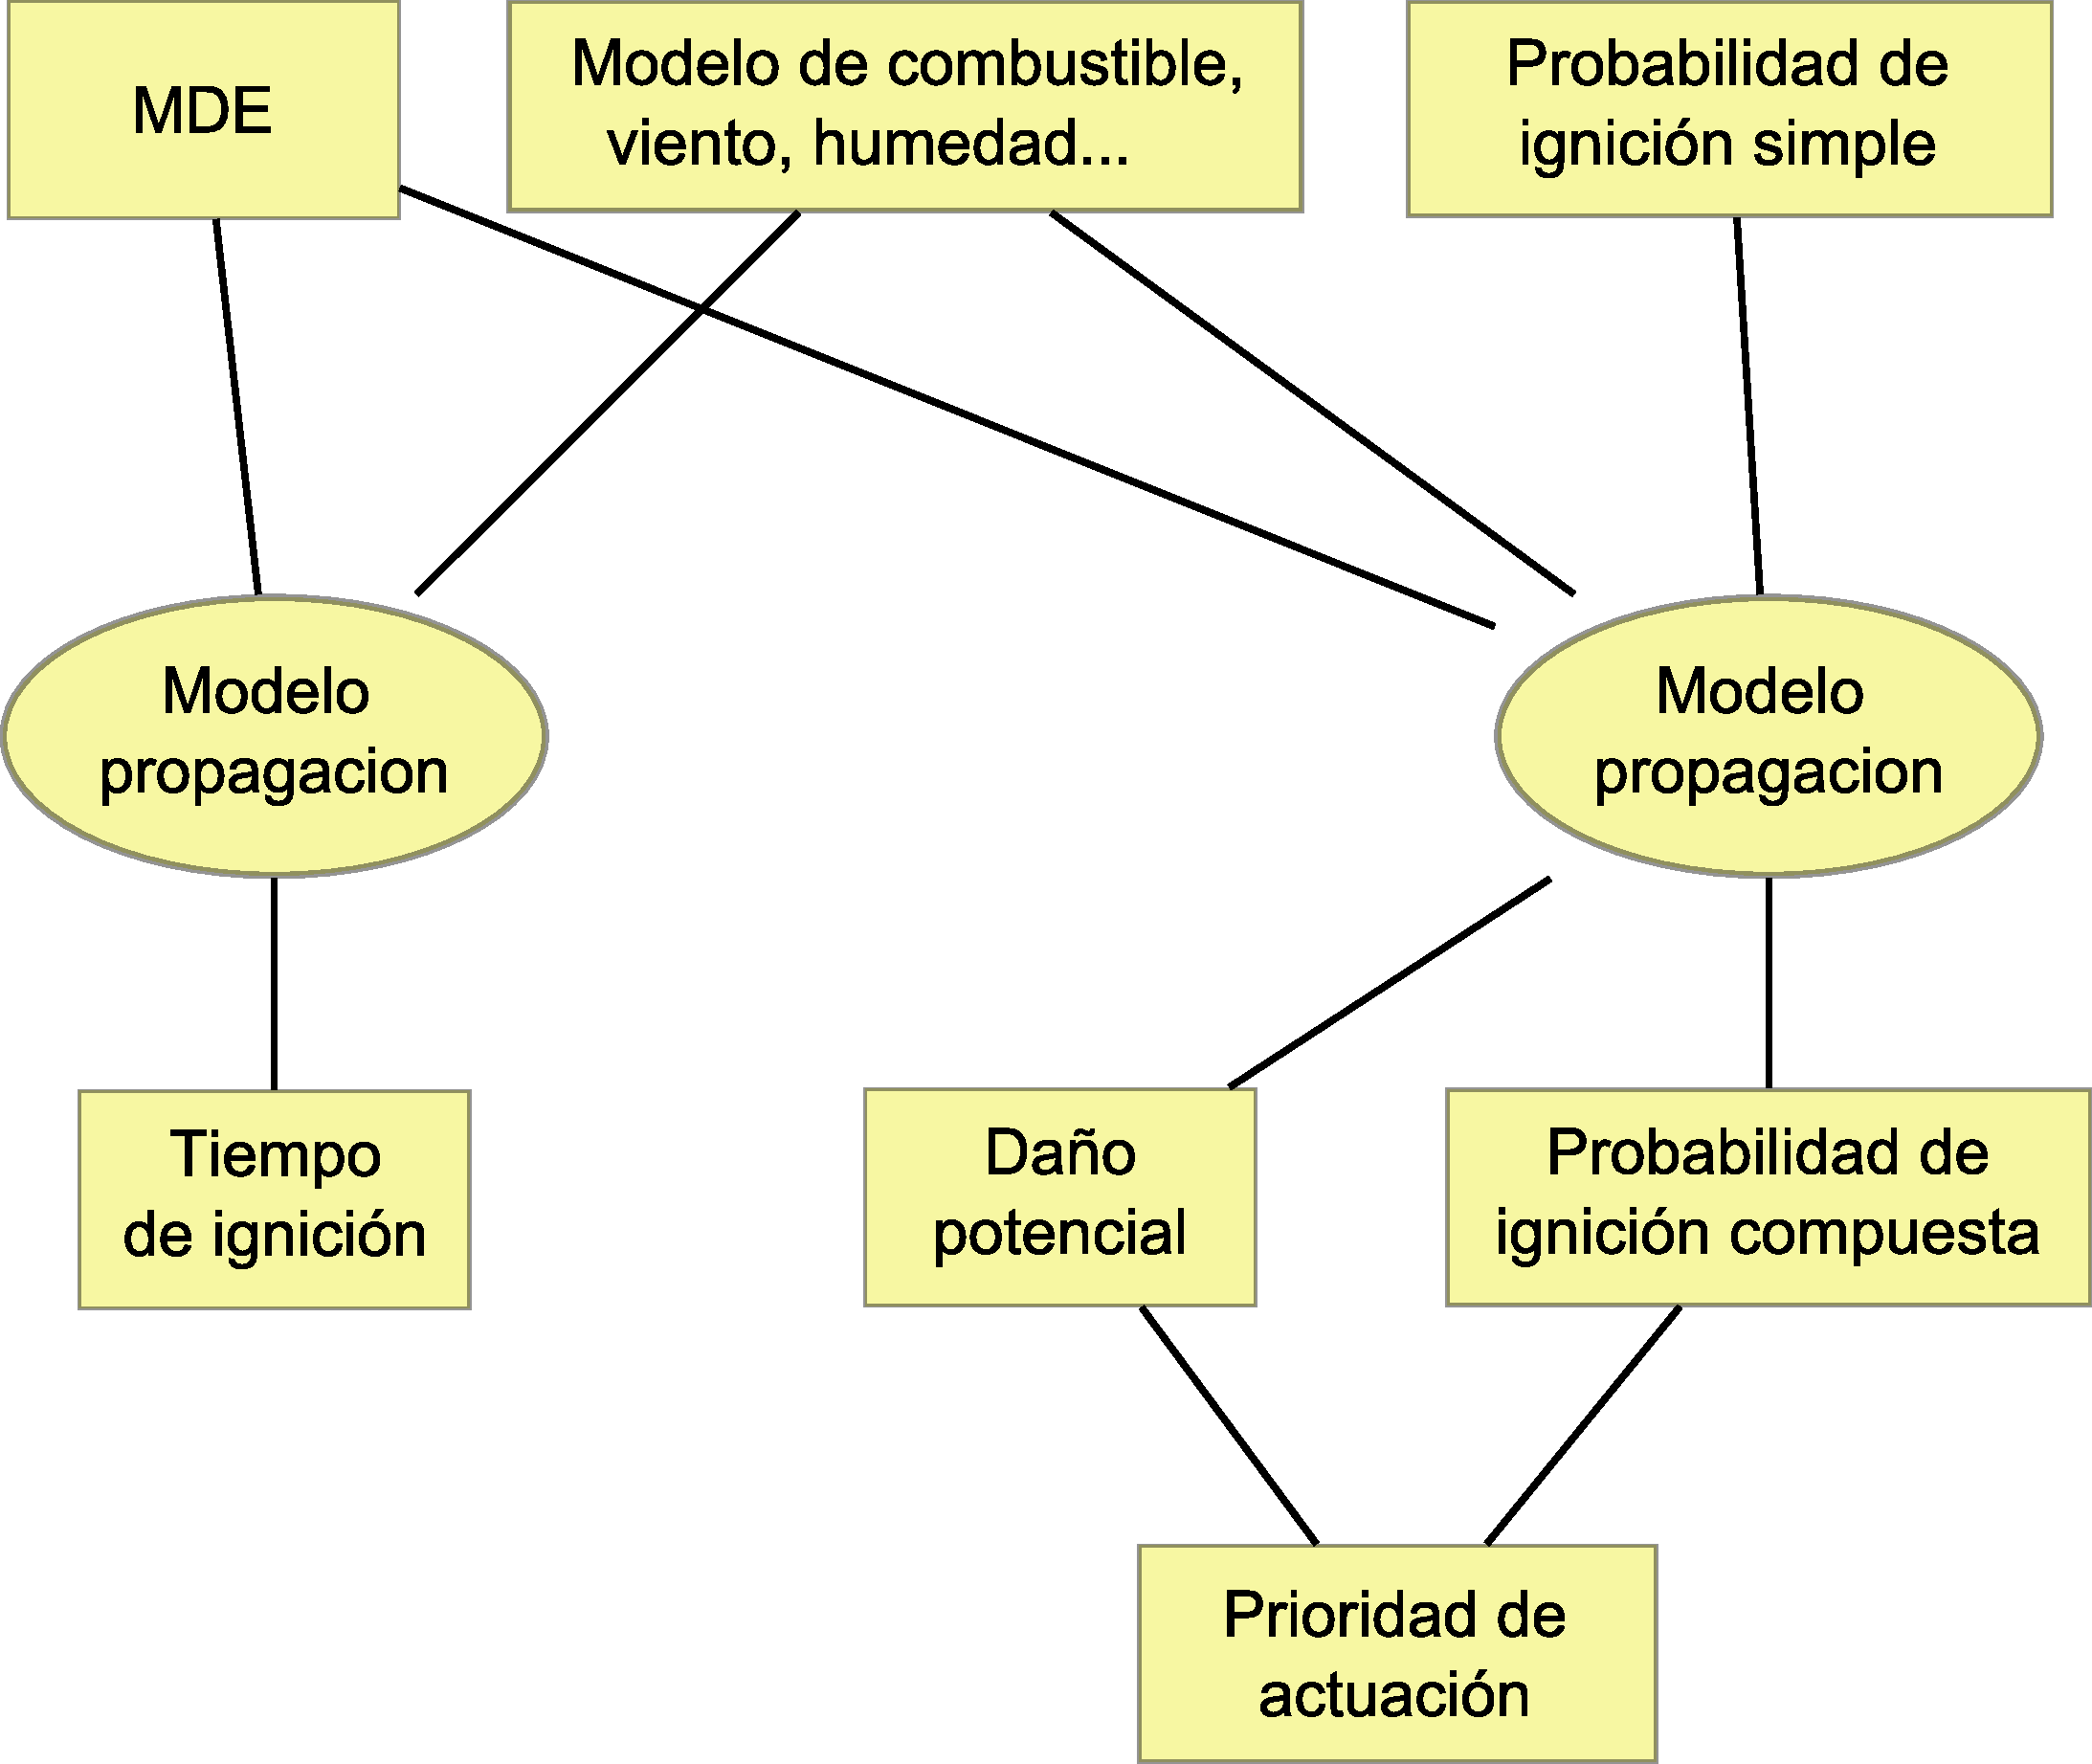
\includegraphics[width=.5\textwidth]{Analisis_riesgos/Esquema_riesgo_incendio.pdf}
\caption{\small Esquema funcional del an�lisis de riesgo de incendios.}
\label{Fig:Esquema_riesgo_incendio}
\end{figure}

\subsection{Apoyo en tareas relacionadas con riesgo de incendios}

La gesti�n de incendios y sus riesgos asociados incluye otra serie de tareas adem�s de las anteriores, siendo el SIG de gran utilidad para la mayor parte de ellas.

Como hemos visto, el estudio de riesgos combinado con la modelizaci�n nos permite obtener resultados en base a los cuales pueden establecerse prioridades de asignaci�n, Esto constituye una ayuda para decidir, por ejemplo, en qu� zonas resulta de inter�s centrar las labores de vigilancia. Situar los elementos necesarios para llevar a cabo esta labor no es, sin embargo, una labor inmediata, y optimizar su localizaci�n es una tarea de an�lisis espacial que un SIG puede desarrollar de forma inmejorable.

Las formulaciones que vimos en el cap�tulo \ref{Geomorfometria} relativas a visibilidad sirven para emplazar torres de vigilancia de la forma m�s adecuada, garantizando que el �rea que puede vigilarse desde estas sea la mayor posible. De igual modo, estos an�lisis permiten garantizar que el emplazamiento de una de tales torres cubre una zona de especial relevancia, o cualquier otra cuesti�n similar.

El trabajo de detecci�n y gesti�n de incendios se ve tambi�n ayudado por el SIG. Una vez localizado el incendio desde varias torres, la posici�n exacta de este puede calcularse por triangulaci�n, un procedimiento sencillo que se lleva a cabo de forma r�pida en un SIG. 

Aunque m�s novedosas e implementadas por el momento en menor medida, otras tecnolog�as de tipo SIG pueden adaptarse para su uso por parte de los t�cnicos encargados de las labores de vigilancia y control de operativos, as� como por los propios equipos que trabajan en campo. Las tecnolog�as Web facilitan la comunicaci�n entre todos los profesionales implicados en la lucha contra incendios, y si estas tecnolog�as incorporan elementos SIG multiplican su utilidad para todos ellos.  En \cite{Domez2008Girona} puede encontrarse una interesante propuesta tecnol�gica al respecto.

Por su parte, los SIG montados sobre dispositivos m�viles pueden aumentar las posibilidades de trabajo y coordinaci�n, ampliando el nivel de conocimiento del que las cuadrillas de extinci�n disponen en cada momento acerca del incendio.

En el nivel de control, la gesti�n de los efectivos que trabajan en las labores de extinci�n puede hacerse tambi�n desde un SIG, trabaj�ndose en tiempo real con las distintas variables tales como la extensi�n del incendio o el emplazamiento de los equipos en campo. 

En relaci�n con la situaci�n de los equipos, tecnolog�as relacionadas con los SIG como los Sistemas de Posicionamiento Global permiten un r�pido avance hasta las zonas de actuaci�n, facilitando la localizaci�n de estas. Si estos equipos est�n conectados a su vez con un elemento central que los gestione, y este incorpora funcionalidades SIG, se tiene un sistema completo para el control de las tareas de extinci�n, el cual a su vez permite an�lisis adicionales en tiempo real. El resultado es una gesti�n m�s eficaz e integrada, en la cual el SIG juega un papel central.

Una tecnolog�a de gran importancia tanto para la detecci�n como para el seguimiento de incendios es la teledetecci�n. Los productos de la teledetecci�n tienen una aplicaci�n directa en ambas tareas, y existen an�lisis particulares que pueden emplearse tanto para localizar puntos en los que se inicie un incendio (y a partir de ello, proceder a organizar las respectivas labores de combate), o seguir el avance de este.

Los fundamentos principales del uso de im�genes de sat�lite para detecci�n de incendios residen en el an�lisis de la informaci�n que estas pueden ofrecer acerca de la temperatura del terreno. Especialmente relevante para esta tarea es la banda del infrarrojo t�rmico, pues las emisiones debidas a la temperatura del cuerpo se presentan en la longitud de onda correspondiente a dicha banda. Este planteamiento ha sido desarrollado abundantemente\cite{Chuvieco1990PEARS, Ellyett1974RSE}, y su aplicaci�n ha demostrado la gran utilidad de las im�genes de sat�lite para estas tareas. El uso de la banda del infrarrojo medio tambi�n es otra posibilidad \cite{Robinson1991IJRS}, aunque menos habitual.

Aunque puede utilizarse cualquier sensor cuyos productos incluyan una banda en la zona del infrarrojo t�rmico, es particularmente popular el uso del sensor AVHRR, cuya banda 3 (3,55--3,93$\mu$m) es adecuada para este tipo de an�lisis.

La clasificaci�n de los p�xeles en funci�n de la temperatura extra�da de la banda del infrarrojo t�rmico arroja, no obstante, falsos positivos en muchos casos, e indica como p�xeles incendiados algunos que no lo son. Para filtrar los resultados, pueden aplicarse formulaciones adicionales como el an�lisis de los p�xeles vecinos tanto en la propia banda del infrarrojo t�rmico como en otras.

\section{Resumen}

El an�lisis de riesgos representa una importante �rea de aplicaci�n de las tecnolog�as SIG.

Uno de los an�lisis fundamentales es el de riesgos climatol�gicos, el cual aplica las herramientas de an�lisis y modelizaci�n climatol�gica. Estas pueden aportar informaci�n sobre la situaci�n clim�tica en un instante concreto (modelizaci�n cartogr�fica del clima), o bien sobre el comportamiento del clima a lo largo de un periodo dado (modelizaci�n din�mica del tiempo).

Los resultados de este an�lisis son el punto de partida para otros, muy especialmente los relacionados con la hidrolog�a, tales como inundaciones o aludes. En ambos casos, el SIG representa una herramienta de gran utilidad para la preparaci�n de las variables necesarias para el an�lisis, y en la actualidad se integra con aplicaciones externas que son las encargadas de llevar a cabo los procesos de modelizaci�n correspondientes. Los resultados de esta modelizaci�n (�reas de inundaci�n, �reas potencialmente afectadas por avalanchas, etc.) pueden posteriormente ser visualizados y analizados dentro de un SIG.

Otros riesgos tales como los desplazamientos en masa se pueden estudiar y cartografiar exclusivamente con el uso de un SIG, ya que dependen en su mayor�a del propio terreno, siendo un SIG una excelente herramienta para el an�lisis de Modelos Digitales de Elevaciones y la extracci�n de par�metros derivados.

Por �ltimo, hemos visto en este cap�tulo c�mo puede modelizarse el comportamiento de un incendio con un Sistema de Informaci�n Geogr�fica. Empleando los fundamentos de esa modelizaci�n, se obtienen variables derivadas tales como cartograf�a de riesgos de incendio. 

Las tecnolog�as SIG son tambi�n relevantes en el campo de la lucha directa contra incendios, no ya mediante esos procesos de modelizaci�n y an�lisis, sino como herramienta soporte para las tareas relacionadas con la extinci�n y gesti�n de equipos de combate.

%\bibliographystyle{unsrt}
%\bibliography{../../Libro_SIG}

%\chapter{Ciencias sociales}
\label{Ciencias_sociales}



\bigskip

\begin{intro}
Aunque los SIG nacieron como herramientas vinculadas al estudio del medio natural, muchas otras disciplinas han sabido sacar tanto o m�s partido de ellos que las propias ciencias del medio. Entre ellas, las ciencias sociales hacen un uso muy diverso y rico de los SIG, pues todas ellas incluyen en alg�n punto alguna componente geogr�fica en cuyo an�lisis los SIG pueden ser herramientas de primer orden.

En este cap�tulo estudiaremos esos usos y veremos la versatilidad de los SIG para aplicaciones de toda �ndole, desde sencillos modelos demogr�ficos a aplicaciones en arqueolog�a, donde las necesidades del estudio del tiempo como variable fundamental hacen necesarios elementos de un SIG muy distintos.
\end{intro}

%\bibliographystyle{unsrt}
%\bibliography{../../Libro_SIG}
\chapter{Ecolog�a}
\label{Ecologia}



\bigskip

\begin{intro}
Los SIG son herramientas b�sicas para bi�logos y otros profesionales que analizan las comunidades animales o vegetales, o cualquier otro elemento del medio natural. Trat�ndose de elementos vivos y din�micos, presentan casos de uso interesantes para demostrar las capacidades de los SIG de cara al estudio de su evoluci�n y desarrollo a lo largo del tiempo.

En este cap�tulo detallaremos algunas formulaciones particulares que estas disciplinas aportan a los SIG, y el uso que de ellas se hace en las situaciones y aplicaciones m�s habituales .
\end{intro}

\section{Introducci�n}

Los SIG son herramientas b�sicas en la actualidad dentro del campo de la ecolog�a, algo que no deber�a resultar extra�o teniendo en cuenta la importancia de la informaci�n geogr�fica en este �mbito. Del mismo modo que la cartograf�a ha sido una parte fundamental para el estudio del medio natural y de las comunidades animales y vegetales, con la aparici�n de los SIG estas tareas han pasado a adoptar todas las funcionalidades de estos, al tiempo que las han aprovechado para desarrollar nuevas formas de explotar la informaci�n geogr�fica.

El uso que se hace de los SIG en el campo de la ecolog�a es en buena parte anal�tico, tratando de extraer informaci�n a partir de los datos de que se dispone, ya sean estos acerca del medio, de una especie dada o de una comunidad natural de cualquier tipo. Este volumen de datos es, no obstante, grande en muchos casos, y el uso de SIG permite una gesti�n adecuada y, muy especialmente, una presentaci�n �ptima de estos. Mientras que el an�lisis es una labor m�s t�cnica, la ecolog�a genera productos de inter�s para un p�blico menos especializado, y mostrar a este los resultados de esos an�lisis o bien los datos de partida directamente a trav�s de cartograf�a es una soluci�n id�nea en la que los SIG se demuestran de gran ayuda. 

Veremos en este cap�tulo dos bloques de conocimiento significativos dentro del uso que se le da a los SIG en el terreno de la ecolog�a. Por una parte, la arquitectura del paisaje, un tipo de an�lisis en el que fundamentalmente se estudian las formas y patrones espaciales de los distintos elementos que forman un entorno natural o paisaje. Es decir, un an�lisis de c�mo est� compuesto espacialmente ese paisaje. Por otra, veremos los denominados \emph{modelos predictivos}, que conforman un an�lisis estad�stico m�s centrado en la componente tem�tica de la informaci�n geogr�fica. Al aplicarlos en un contexto espacial, nos van a permitir la elaboraci�n de cartograf�a de potencialidad, �til como veremos para diversas tareas.


\section{Ecolog�a del paisaje}


En ecolog�a se entiende por paisaje a un entorno natural dado, con unas caracter�sticas concretas fruto de la interacci�n de m�ltiples factores como el clima, la presencia humana, las comunidades animales y vegetales, o el relieve, entre otros. No se trata, por tanto, del concepto est�tico de paisaje como lo entendemos en su acepci�n habitual, sino un concepto geogr�fico y ecol�gico que hace referencia a c�mo todos esos elementos que act�an sobre una porci�n de terreno definen sus caracter�sticas.

\index{Ecolog�a del paisaje}

El resultado de todas esas acciones es un conjunto heterog�neo de unidades que ponen de manifiesto la forma distinta en que sobre las distintas partes del paisaje act�an los elementos que le dan forma. No es dif�cil ver que esta heterogeneidad es una heterogeneidad espacial, y que las fuerzas que la originan tambi�n tienen un car�cter espacial igual, por lo que su estudio y an�lisis es susceptible de aprovecharse en gran medida de las capacidades de un SIG.

El estudio del paisaje definido seg�n lo anterior conforma la denominada \emph{ecolog�a del paisaje}, una disciplina que analiza tanto la estructura como el funcionamiento del paisaje como entidad. SIG y ecolog�a del paisaje van �ntimamente unidas desde los inicios de ambas disciplinas, y del conjunto de t�cnicas que se utilizan para el estudio del paisaje, una buena parte han sido desarrolladas sobre la base del SIG como herramienta a emplear para su aplicaci�n.

Seg�n \cite{Forman1983Bioscience}, la ecolog�a del paisaje es el <<estudio de las interacciones entre los aspectos temporales y espaciales del paisaje y sus componentes de flora, fauna y culturales>>. Este estudio se puede entender como suma de tres tipos distintos de an�lisis:


\begin{itemize}
	\item An�lisis de las propiedades espaciales de las unidades del paisaje y sus relaciones espaciales. Estas unidades forman <<manchas>> sobre el conjunto total del paisaje, y la forma en que estas se distribuyen sobre el terreno condiciona muchos aspectos del paisaje cuyo estudio es altamente relevante, as� como las caracter�sticas espaciales de cada una, tales como su forma o el �rea que ocupan.
	\item An�lisis de la interacci�n entre las unidades. Cada unidad no es un elemento estanco, y se producen flujos entre ellas que tambi�n son de inter�s para su caracterizaci�n y la del paisaje como entidad global.
	\item An�lisis de la din�mica temporal del paisaje. Es decir, de la evoluci�n de ese conjunto de unidades a lo largo del tiempo y los cambios que se producen en su estructura.
\end{itemize}

De cara a su estudio en un SIG, el primer punto de los anteriores es el que tiene mayores posibilidades de aprovechar las capacidades de este, puesto que se trata de un an�lisis netamente espacial. Los otros dos, no obstante, tambi�n pueden llevarse a cabo en un SIG. Aunque no los veremos aqu� y nos centraremos en el estudio de las relaciones espaciales, en el apartado \ref{Cambio_usos_suelo} detallaremos los modelos de cambio de usos del suelo, cuyos fundamentos son aplicables de igual modo para estudiar el cambio en las unidades del paisaje. Estos modelos, de hecho, constituyen herramientas para el estudio del paisaje, ya que el uso de suelo es un factor m�s de la caracterizaci�n de las unidades paisaj�sticas.

El an�lisis de las relaciones espaciales entre las unidades del paisaje persigue obtener una caracterizaci�n cuantitativa de este, y lleva esto a cabo analizando diferentes propiedades espaciales de las unidades por separado, as� como de cada una junto a las circundantes, y a nivel global de todo el paisaje. Esto permite obtener resultados que pueden relacionarse con cada una de las funciones que las unidades de paisaje cumplen, y dar una caracterizaci�n de este a distintas escalas. Por su propia naturaleza, el estudio del paisaje es un �mbito en el que el concepto de escala de an�lisis es vital para que los resultados tengan sentido.

Toda la informaci�n que se maneja en el estudio espacial de las unidades del paisaje es de tipo categ�rico, ya que no nos interesan (al menos con car�cter fundamental) las caracter�sticas de esas unidades, sino saber qu� unidades hay y los l�mites de cada una. Aunque la informaci�n categ�rica resulta en general m�s conveniente manejarla en forma vectorial (como pol�gonos en este caso), el car�cter anal�tico de las tareas que se van a desarrollar hace que el modelo r�ster sea m�s id�neo desde ese punto de vista. Asimismo, las capas categ�ricas a emplear se obtienen frecuentemente mediante t�cnicas de clasificaci�n a partir de im�genes, con lo que originalmente se crean como capas r�ster. Por todo esto, la aplicaci�n de las formulaciones que seguidamente veremos puede encontrarse tanto sobre una base r�ster como sobre una base vectorial, siendo ambas alternativas posibles.

En esencia, y de un modo muy simplista, podemos decir que la labor que vamos a realizar con un SIG para el estudio del paisaje consiste en el an�lisis de los patrones que aparecen en un mapa con informaci�n categ�rica, y la definici�n de las caracter�sticas de cada unidad y de cada categor�a de las presentes. Este an�lisis puede enfocarse desde dos concepciones te�ricas distintas:

\begin{itemize}
	\item La Biogeograf�a de Islas \cite{MacArthur1967Princeton}. Considera cada unidad como una isla, en el sentido de que en su interior puede darse alg�n tipo de proceso ecol�gico, mientras que en las �reas que la rodean el terreno es <<hostil>> para este. Este modelo supone por tanto una concepci�n dicot�mica del paisaje al analizar una unidad o una clase dada. Esto permite un an�lisis sencillo, centrado en las caracter�sticas propias de cada una de esas unidades (las islas) frente al fondo formado por el resto de estas (el <<mar>>). No obstante, es un enfoque que implica una simplificaci�n excesiva, y que no tiene en cuenta la interacci�n entre las unidades ni las caracter�sticas del fondo.
	\item El modelo del mosaico paisaj�stico. Se considera el paisaje como un conjunto de unidades interconectadas y se tiene en cuenta la heterogeneidad de estas. En lugar de enfocar el estudio sobre las unidades en s�, lo hace sobre un proceso dado y sobre c�mo este tiene lugar para un paisaje con una configuraci�n y unas propiedades dadas. Es un modelo m�s real que el anterior, ya que la respuesta de los organismos sobre un tipo de unidad de paisaje no es en realidad �nicamente de dos tipos posibles (isla o mar), sino que pueden existir t�rminos intermedios.
\end{itemize}

\index{Biogeograf�a de Islas}

El n�mero de par�metros que se han definido para el an�lisis cuantitativo del paisaje (conocidos como \emph{m�tricas} del paisaje) es muy elevado, y veremos a continuaci�n solo algunos. El lector interesado en profundizar en el tema puede consultar \cite{fragstatsMetrics}. Para una definici�n completa de todas estas m�tricas, la referencia a consultar es \cite{fragstatsMetricsDefinition}.\index{Metricas@M�tricas (paisaje)}

Las m�tricas del paisaje pueden clasificarse seg�n dos criterios: la escala a la que se aplican y el tipo de propiedades que describen. Seg�n la escala encontramos tres tipos:

\begin{itemize}
	\item Metricas de unidad\footnote{\emph{Patch metrics}, traducido en ocasiones como \emph{m�tricas de parche}, aunque no emplearemos aqu� esta traducci�n}. Analizan las unidades del paisaje de forma independiente del resto.
	\item M�tricas de clase. Analizan las manchas que corresponden a una misma clase, es decir, un conjunto de pol�gonos disjuntos con las mismas caracter�sticas.
	\item M�tricas del paisaje. Analizan el paisaje en su totalidad, como un conjunto de manchas que teselan el espacio.
\end{itemize}

Las m�tricas de unidad o de clase pueden integrarse para dar informaci�n global del paisaje mediante el uso de estad�sticos tales como la media, la media ponderada, la desviaci�n t�pica o el rango del conjunto de manchas o clases, seg�n corresponda. 

En referencia a las propiedades que describen, los siguientes son los grupos principales:

\begin{itemize}
	\item M�tricas de composici�n. Se aplican tan solo para el paisaje globalmente y reflejan la forma en que las distintas clases est�n representadas en este.
	\item M�tricas de configuraci�n. Se aplican a los distintos niveles de escala y recogen la configuraci�n espacial de las distintas unidades. 
\end{itemize}\index{Composici�n, m�tricas de}\index{Configuraci�n, m�tricas de}

Veremos algunos de los principales representantes de estos dos grupos a continuaci�n. 

\subsection{M�tricas de composici�n}

Las m�tricas de composici�n estudian la variedad y la abundancia de las distintas clases dentro del paisaje. Algunas de las principales m�tricas de este tipo son las siguientes:

\begin{itemize}
	\item Abundancia. La abundancia es uno de los par�metros m�s sencillos de calcular, pero que m�s informaci�n aporta acerca del paisaje. Simplemente se expresa como el porcentaje de �rea que cada clase supone en el total del paisaje.
	\item Riqueza. La riqueza indica el n�mero total de clases distintas que el paisaje contiene. Pese a ser tambi�n un par�metro de gran simpleza, su significado es muy importante para la caracterizaci�n del paisaje. Por ejemplo, y puesto que muchos organismos se asocian con un tipo concreto de clase (un h�bitat particular definido por esta), puede asumirse que una mayor riqueza en t�rminos de estas clases supone a su vez una mayor riqueza en lo que a especies respecta. \index{Riqueza}\index{Abundancia}
	
	La riqueza tiene una relaci�n directa con la escala, ya que �reas mayores presentan mayor heterogeneidad, lo que se traduce en mayor riqueza. Comparar la riqueza de paisajes de diferente tama�o puede ser, por tanto, problem�tico.
	
	Su propia simplicidad es tambi�n el principal punto d�bil de est� m�trica, ya que un paisaje compuesto por 3 clases distintas representadas cada una por un 33\% de la superficie no es igual que un paisaje en el que una de ellas ocupara un 98\% y las restantes un 1\% cada una. Aunque los valores de riqueza sean los mismos, la estructura de las comunidades animales y vegetales ser� muy distintas en ambos casos, por lo que la informaci�n a este respecto que puede inferirse debe considerarse en conjunto con otras m�tricas que aporten informaci�n adicional, tales como las detalladas a continuaci�n.
		
	\item Equitatividad. La equitatividad es el concepto contrario a la dominancia. En un paisaje existe equitatividad cuando todas las clases se encuentran representadas de igual modo. Por el contrario, si una de ellas ocupa un �rea mayor que las restantes (como en el caso citado anteriormente), existe dominancia de esta. Existen varios �ndices que miden la equitatividad, entre los que destacan los dos siguientes:\index{Equitatividad}\index{Dominancia}
	
\begin{itemize}
	\item �ndice de equitatividad de Shannon. Se calcula seg�n la expresi�n
	\begin{equation}
E = -\frac{\sum_{i=1}^{s}{P_i\ln{P_i}}}{\ln{s}}
\end{equation}
\noindent siendo $s$ el n�mero total de clases presentes y $P_i$ la proporci�n ocupada por la clase i--esima en el paisaje.
	\item �ndice de equitatividad de Simpson. Seg�n la expresi�n
	\begin{equation}
E = \frac{1-\sum_{i=1}^{n}{P_i^2}}{1 - \frac{1}{n}}
\end{equation}
\noindent donde $n$ es el n�mero total de clases.
\end{itemize}
	En ambos casos, la dominancia puede calcularse como $1 - E$.
	
	Ambos �ndices var�an de 0 a 1.
	
\index{Indice@�ndice!de equitatividad}
	\item Diversidad. La diversidad tiene relaci�n con la equitatividad y la riqueza, y se calcula en funci�n de estas variables de diversas formas, seg�n sea la importancia asignada a cada una de ellas. Algunas de las f�rmulas m�s comunes son las siguientes:\index{Diversidad}
	
\begin{itemize}
\item �ndice de diversidad de Shannon. El m�s usado, responde a la expresi�n
	\begin{equation}
H = -\sum_{i=1}^{s}{P_i\ln{P_i}}
\end{equation}

	\item �ndice de diversidad de Simpson. Calculado seg�n la siguiente expresi�n:
		\begin{equation}
D = 1-\sum_{i=1}^{n}{P_i^2}
\end{equation}
\index{Indice@�ndice!de diversidad}
\end{itemize}

Puede verse que los �ndices de diversidad corresponden al numerador de los de equitatividad presentados anteriormente. El denominador es el valor de la diversidad m�xima.

\end{itemize}

\subsection{M�tricas de configuraci�n}

Las m�tricas de configuraci�n son m�s abundantes que las de composici�n, a la vez que m�s variadas. Las siguientes son algunas de las caracter�sticas que pueden cuantificarse mediante este tipo de m�tricas.

\begin{itemize}
\item Tama�o. El par�metro m�s b�sico, empleado a su vez como parte de otras m�tricas. Pueden calcularse estad�sticos del tama�o de unidad para todo el paisaje o bien para una clase dada. Tambi�n puede emplearse como densidad, expresando el n�mero de distintas unidades por unidad de �rea.
\item Complejidad de forma. Existen muchas m�tricas en este grupo, la mayor�a de las cuales intentan describir la complejidad de la forma geom�trica de la unidad. En muchos casos esto se lleva a cabo mediante relaciones per�metro/�rea, y comparando estas con las correspondientes a una figura geom�trica regular (circulo o cuadrado generalmente) de la misma �rea. Aunque la forma de la unidad puede relacionarse con el comportamiento de ciertas especies animales y vegetales (actividad, migraci�n, colonizaci�n de la unidad, etc.), la principal implicaci�n de estos par�metros es en relaci�n con el efecto de borde (recu�rdese lo visto en \ref{EfectoBorde}). La dimensi�n fractal de la unidad es tambi�n un par�metro empleado con frecuencia. Otras m�tricas m�s elaboradas pueden calcularse igualmente, aunque la interpretaci�n de su significado en t�rminos ecol�gicos no es tan clara.\index{Efecto!de borde}\index{Dimensi�n!fractal}\index{Complejidad de forma}
\item Bordes. Adem�s de la relaci�n directa que guarda con las m�tricas de complejidad de forma, el efecto de borde puede medirse directamente con otras m�tricas. La m�s simple de todas ellas es la mera longitud total de los bordes, es decir, de los per�metros de las distintas unidades, ya sea de forma individual o agrupadas por clases o paisaje total. Tambi�n puede expresarse como densidad, en longitud de borde por unidad de de �rea.
\item �rea central. Estas m�tricas tratan de cuantificar el �rea de la unidad libre de efecto de borde. Para ello, se elimina un �rea dada situada a una distancia del borde menor que un umbral establecido, y se cuantifica el �rea restante. Estas m�tricas integran la complejidad de la forma, el �rea y los efectos de borde en un �nico valor descriptivo. Se entiende que esta �rea central es la que es de inter�s para el estudio de ciertos procesos o el comportamiento de una comunidad concreta.
\item Aislamiento/proximidad. Las m�tricas de esta clase cuantifican la tendencia de las unidades de una misma clase a aparecer en el paisaje cercanas entre s� o bien separadas. Una forma de llevar esto a cabo es mediante el c�lculo de la distancia al vecino m�s cercano, es decir, a la mancha de paisaje de la misma clase que se encuentra a una distancia menor. Estas distancias para cada unidad de una clase pueden promediarse, ya sea asignando peso a cada una en funci�n del �rea correspondiente a la unidad en cuesti�n, o bien considerando el mismo peso para todas.\index{Aislamiento}

Como es l�gico pensar, este c�lculo de las distancias entre unidades no se lleva a cabo de la misma manera si trabajamos con datos r�ster o vectoriales, y las formulaciones difieren notablemente. Conservan, no obstante, la misma base te�rica, y la interpretaci�n de los resultados es id�ntica.
	\item Conectividad. La conectividad cuantifica el grado en que el paisaje impide o facilita el flujo entre las distintas unidades. La p�rdida de conectividad es una de las razones m�s importantes para la p�rdida de h�bitat. Si el h�bitat se fragmenta y no existe conexi�n entre las distintas comunidades de una especie, esto puede llevar a un menor n�mero de individuos en cada unidad de las habitadas por dicha especie, y en �ltima instancia incluso causar su extinci�n.\index{Conectividad}
	
	Para estudiar la conectividad, es fundamental definir qu� condiciones han de cumplir dos unidades de una clase dada para considerarse como conectadas, lo cual depende del proceso que pretendamos estudiar, as� como del resto de unidades. Se ha de trabajar con una \emph{conectividad funcional} entre unidades. La distancia es un par�metro fundamental a considerar, sin duda, aunque no el �nico. Una distancia insalvable para un peque�o reptil puede no constituir un problema para un ave o para la dispersi�n de las semillas de un �rbol. Asimismo, para una especie que habite en un h�bitat boscoso, cruzar una determinada distancia de pasto puede ser perfectamente viable, mientras que una distancia menor ocupada por agua puede constituir una barrera insalvable que no permite que exista conectividad.
	
	El conjunto de unidades y sus conexiones funcionales constituye una red que puede analizarse con algunas de las ideas que ya conocemos a este respecto, as� como definirse con par�metros derivados de la teor�a de grafos (Figura \ref{Fig:Conectividad}).\index{Teor�a de grafos}
	
\begin{figure}[!hbt]      
\centering
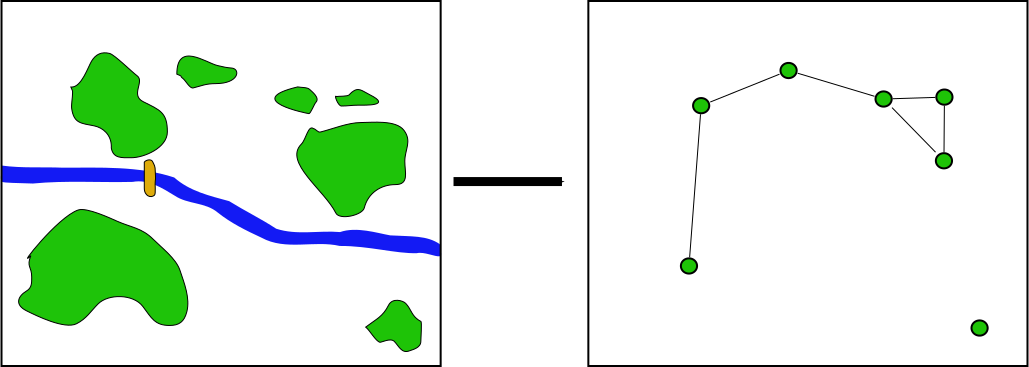
\includegraphics[width=\textwidth]{Ecologia/Conectividad.pdf}
\caption{\small Para el an�lisis de conectividad, el conjunto de unidades de una clase se convierten en una red que define la conectividad funcional entre ellas.}
\label{Fig:Conectividad}
\end{figure}

	\item Contraste. El contraste cuantifica la diferencia relativa entre cada unidad y las contiguas. Una zona de bosque rodeada de una zona de pasto no constituye el mismo tipo de paisaje que esa misma zona rodeada de �reas urbanas o de agua. Una forma de calcular m�tricas de contraste es aplicar las ideas de las m�tricas de borde, pero asignando pesos a estos en funci�n de la diferencia que exista entre las dos unidades que cada borde delimita.
	\item Contagio. El contagio expresa la tendencia de las unidades de una clase a formar grupos compactos, o bien a estar dispersas a los largo del paisaje.\index{Contraste}\index{Contagio}
\end{itemize}

\subsection{\emph{Software}}

Sin duda alguna, el software m�s extendido para el an�lisis del paisaje es FRAGSTATS \cite{referenciaFragstats}, referencia en su campo y del que derivan la mayor parte de par�metros que acabamos de ver. Existen otras aplicaciones que toman elementos de FRAGSTATS e implementan parte de las m�tricas que este calcula (muchas de ellas son sumamente sencillas y su implementaci�n no es costosa), y algunos SIG incluyen funcionalidades de an�lisis basadas en esas ideas. No obstante, es habitual encontrar componentes en algunos de los SIG m�s habituales que permiten usar FRAGSTATS directamente desde esos SIG.

Como aplicaci�n, FRAGSTATS no es un SIG, aunque dispone de capacidades para leer capas de entrada tanto r�ster como vectoriales en formatos que tambi�n pueden leerse en buena parte de los SIG de escritorio m�s populares. La interfaz es sencilla de emplear, pero no existen elementos como los que encontramos en uno de esos SIG para el manejo de capas. La figura \ref{Fig:FRAGSTATS} muestra la interfaz de ajuste de par�metros de FRAGSTATS como aplicaci�n independiente.\index{FRAGSTATS}

\begin{figure}[!hbt]      
\centering
\includegraphics[width=.5\textwidth]{Ecologia/Fragstats.png}
\caption{\small Interfaz de FRAGSTATS}
\label{Fig:FRAGSTATS}
\end{figure}

Las soluciones que enlazan FRAGSTAT con alg�n SIG permiten que pueda ejecutarse el programa directamente desde el SIG, aliment�ndolo con las capas abiertas en este en un momento dado, y completando esta informaci�n con los par�metros que se requieran para la ejecuci�n, introducidos en interfaces dise�adas a tal efecto.

Los resultados generados por FRAGSTATS son en su gran mayor�a en forma de tablas, y es habitual que, una vez el programa ha terminado su trabajo, el SIG a trav�s de su componente de enlace tome esas tablas y las introduzca en �l de la manera m�s conveniente, o al menos facilite desde su interfaz la consulta de estas.

Esta integraci�n dentro de un SIG permite combinar las m�tricas del paisaje con algunas de las posibilidades adicionales que ofrece un SIG. De especial relevancia resultan las capacidades de modelizaci�n, ya que puede modelizarse la evoluci�n del paisaje y caracterizar cada una de las etapas mediante las correspondientes m�tricas. Veremos en el apartado \ref{Cambio_usos_suelo} algo m�s acerca de este tipo de modelizaci�n.

Algunas aplicaciones m�s particulares para el an�lisis del paisaje se centran en determinados aspectos de la caracterizaci�n de este. Por ejemplo, \emph{Conefor Sensinode} \cite{Saura2009EMS} es una aplicaci�n para el an�lisis de la conectividad basada en un uso avanzado de elementos de la teor�a de grafos, as� como para el estudio de la disponibilidad de h�bitats.\index{Conefor Sensinode}

\section{Modelizaci�n de h�bitats. Modelos predictivos}
\label{Modelos_predictivos}

Uno de los an�lisis m�s interesantes en el campo de la ecolog�a, y en el que los SIG aportan mayores posibilidades, es la modelizaci�n de h�bitats. Este tipo de an�lisis pretende establecer qu� tipo de condiciones son las m�s adecuadas para una determinada especie animal o vegetal, y con ello poder establecer en qu� zonas puede estar presente dicha especie y estimar la probabilidad de encontrarla en ellas teniendo en consideraci�n las condiciones all� presentes. 
\index{Modelo!predictivo}

Este tipo de informaci�n puede ser utilizada para predecir la presencia o ausencia de individuos de la especie en unas zonas de inter�s, para analizar si resulta viable la introducci�n de una especie en una concreta, o incluso para tratar de analizar la distribuci�n pasada de una especie y la evoluci�n que desde entonces ha sufrido dicha distribuci�n.

Es f�cil ver que existen similitudes entre el estudio del paisaje y la modelizaci�n de h�bitats, ya que el paisaje condiciona que una especie pueda o no ocupar una determinada zona, y el �xito con que esto sucede, como de hecho hemos mencionado en el apartado anterior de este cap�tulo. No obstante, el tipo de modelizaci�n que tratamos ahora es muy distinto en su enfoque y metodolog�a, y veremos que se trata de t�cnicas distintas con un objetivo tambi�n diferente en lo que a los resultados buscados respecta.

En general, los modelos de h�bitat que vamos a ver toman una serie de variables que se supone tiene influencia en el comportamiento de la especie, estudian los valores de esas variables en los puntos donde se sabe con certeza que la variable est� presente, y posteriormente intentan en base a esos datos valorar la idoneidad de una serie de zonas para acoger igualmente a dicha especie. Adem�s de usar informaci�n sobre la presencia de una especie en una determinada localizaci�n, pueden emplearse datos de ausencia para indicar aquellos lugares en que la especie no aparezca. No obstante, y mientras que una zona de presencia se puede caracterizar sin ninguna duda como tal, la ausencia puede deberse a que, simplemente, no se ha observado, o bien a alg�n hecho particular ajeno a las variables que se consideran para el an�lisis. Crear registros de ausencia es, en general, una labor dif�cil \cite{Jarvis2005ME}.

El resultado de esta modelizaci�n es una cartograf�a de distribuci�n potencial de la especie estudiada, que nos dice la probabilidad de que esa especie est� presente en los distintos puntos de un �rea analizada, a partir de los datos conocidos para unos emplazamientos concretos (aquellos definidos como puntos de presencia o ausencia, y empleados como entrada del modelo). Estos modelos se conocen como \emph{modelos predictivos} o tambi�n \emph{modelos de idoneidad}.

Formalmente, el modelo es una funci�n de probabilidad $P(i)$, seg�n

\begin{equation}
P(i) = f(x_1,x_2,x_3,\ldots,x_n)
\end{equation}

\index{Funci�n! de probabilidad}

\noindent donde $f$ es la funci�n que asigna la probabilidad de aparici�n de la especie en funci�n de una serie de $n$ variables, y $x_1,x_2,\ldots,x_n$ son los valores de esas variables.

Puesto sobre el contexto de un conjunto de capas con tales variables (puesto que han de cubrir el espacio estudiado, estas ser�n de tipo r�ster preferentemente), el modelo predictivo nos proporciona esa cartograf�a de distribuci�n antes mencionada, sin m�s que aplicarlo sobre todas las celdas de las capas de entrada. La presencia del SIG ha contribuido decisivamente al desarrollo de este tipo de modelos, y el avance que se ha dado en las herramientas SIG ha favorecido la aparici�n de nuevas metodolog�as para la creaci�n de cartograf�a de tipo predictivo.

Si estudiamos la forma de proceder de este tipo de an�lisis, es claro que guarda una gran similitud con los procedimientos estad�sticos que vimos en el apartado \ref{Clasificacion}, donde tratamos los m�todos de clasificaci�n supervisada. Partiendo de un conocimiento acerca de unas localizaciones particulares (en este caso son puntos de presencia/ausencia, entonces eran �reas de entrenamiento), se trata de clasificar las restantes dentro de un marco geogr�fico. La clasificaci�n en este caso ser�a en dos �nicas clases (hay presencia o no de la especie), aunque, puesto que usamos la funci�n de probabilidad, se asemejar�a m�s al tipo de clasificaci�n que denomin�bamos \emph{d�bil}, el cual nos ofrece valores en funci�n de los cuales podemos posteriormente discriminar y establecer si la presencia de la especie puede asumirse o no.\index{Clasificaci�n!supervisada}\index{Clasificaci�n!d�bil}

Las similitudes entre la aplicaci�n de modelos predictivos y t�cnicas de clasificaci�n supervisada no es solo aparente, sino que sus fundamentos son en gran medida los mismos y emplean herramientas de an�lisis comunes. No obstante, un modelo predictivo tiene sus propias caracter�sticas y un objetivo m�s acotado que el de la clasificaci�n gen�rica, por lo que existen algunas diferencias y soluciones particulares, que ser�n las que veamos en esta secci�n. Por ejemplo, el uso de variables cualitativas no es tan habitual en los algoritmos de clasificaci�n (las metodolog�as que fueron explicadas en su momento solo trabajan con variables cuantitativas), mientras que en los modelos predictivos se contempla en algunos de ellos el uso de todo tipo de variables. En general, estos modelos est�n, como parece l�gico, adaptados al hecho particular que modelizan.

A la hora de su operativa dentro de un SIG, usaremos un conjunto de capas r�ster y una capa vectorial de puntos que debe contener un campo que especifique si el punto es de presencia o ausencia. Las capas con las variables independientes pueden ser de todo tipo, y vendr�n condicionadas a las entradas que el modelo requiera. Algunos modelos trabajan con capas cualesquiera y las estudian todas por igual como condicionantes del comportamiento de la especie. Otros exigen una cierta serie de capas concretas, ya que no emplean estas directamente como variables para los an�lisis correspondientes, sino otras intermedias que son calculadas a partir de ellas.

L�gicamente, el uso de unas u otras variables esta condicionado a la escala del estudio a realizar. Un modelo de distribuci�n para una extensi�n grande de territorio puede asumir que el clima es el factor principal a considerar. Para un estudio local, sin embargo, el clima sigue teniendo importancia, pero otras circunstancias han de considerarse igualmente, en especial el relieve \cite{Guisan2000EM}.

\subsection{Algunos modelos de uso frecuente}

Un modelo sencillo es el denominado BIOCLIM \cite{BIOCLIM}, que parte de una serie de par�metros climatol�gicos, asumiendo por tanto que el clima es el �nico factor que condiciona el comportamiento de la especie. Estos par�metros, no obstante, son utilizados para el c�lculo de otras variables biol�gicamente  m�s significativas, y es sobre estas sobre las que se opera. La t�cnica de clasificaci�n de BIOCLIM es en realidad un m�todo de paralelep�pedos como el que vimos en \ref{Paralelepipedos}, ya que calcula el hipercubo delimitado por un umbral $x$, de tal forma que la dimensi�n de ese hipercubo en cada eje es el rango de los valores de la variable correspondiente a dicho eje, recortado en un tanto por ciento $x$. Un valor habitual del umbral es 5\%, de tal modo que la dimension de cada eje se sit�e entre los valores del 5\% y el 95\% del rango para la variable correspondiente.
\index{BIOCLIM}

Se trata de un modelo simple, que sin embargo tiene muchas desventajas debido a las condiciones que asume y a que no permite el uso de variables distintas de las climatol�gicas.

Algo m�s elaborado, aunque tambi�n dentro de la misma familia (ambos modelos solo requieren datos de ausencia), es el modelo DOMAIN, basado en la denominada \emph{distancia de Grover}. Esta tiene la forma\index{Distancia!de Grover}\index{DOMAIN}

\begin{equation}
G_{AB} = \frac{1}{n}\sum_{k=1}^n{\frac{|A_k-B_k|}{\mathrm{rango}(k)}}
\end{equation}

\noindent donde $n$ es el n�mero total de variables, $A_k$ el valor de la variable $k$ en el punto de presencia $A$, $B_k$ el valor de la variable $k$ en la celda $B$ y $\mathrm{rango}(k)$ el rango de la variable $k$ en los puntos de presencia. La media de distancias de Grover entre una celda y todos los puntos de presencia nos da una idea de la diferencia entre estos �ltimos y la celda en cuesti�n. Como estad�stico de similitud puede emplearse el valor $1-G$.

Algunos modelos m�s complejos soportan el uso de datos de ausencia. Entre estos encontramos el modelo Maxent \cite{Phillips2006EM}, que crea �l mismo puntos de pseudo-ausencia. Este modelo se basa en el principio estad�stico de m�xima entrop�a. Otro modelo habitual es GARP (\emph{Genetic Algorithm for Rule set Production}), basado en algoritmos gen�ticos y con un funcionamiento mucho m�s complejo.  Los �rboles de clasificaci�n y regresi�n (\emph{classification and regression trees}, CART)\cite{Breiman1984WB} son otra t�cnica estad�stica que puede aplicarse para desarrollar modelos predictivos. Su uso en un SIG es, sin embargo, complejo \cite{Felicisimo2005Dehesa}, por lo que tienen menos valor a la hora de crear cartograf�a de distribuci�n potencial.\index{CART}\index{GARP}\index{Maxent}\index{Regresi�n!log�stica}

Citar, por �ltimo, el uso de regresi�n log�stica m�ltiple como una alternativa habitual para plantear este tipo de modelos. La probabilidad en este caso viene dada por una f�rmula del tipo

\begin{equation}
P(i) =  \frac{1}{1+e^{b_0 + x_1b_1+x_2b_2+\ldots+x_nb_n}}
\end{equation}

\noindent donde $x_1\ldots x_n$ son los valores de las variables y  $b_1 \ldots b_n$ son constantes.

Para saber m�s sobre estos y otros modelos, puede consultarse \cite{GarciaMateo2008phd}.


\subsection{Validaci�n}

La cartograf�a obtenida mediante la aplicaci�n de los anteriores modelos debe validarse del mismo modo que suced�a en el caso de la clasificaci�n. Tambi�n en este caso se necesita informaci�n complementaria que no haya sido empleada para el modelo, tal como un segundo conjunto de puntos de presencia y ausencia sobre el que contrastar la bondad de los resultados generados.

Las t�cnicas a emplear son tambi�n similares a lo que vimos entonces para la clasificaci�n, comparando aquello que se conoce en los puntos de ese segundo conjunto (si son ausencias o presencias) con lo que el modelo predice. Cruzando estas informaciones se pueden elaborar estad�sticos que ayuden a valorar si el resultado que hemos obtenido es v�lido. Es decir, a valorar la consistencia del modelo.

El �ndice Kappa que ya conocemos es un estad�stico empleado habitualmente, y se aplica de la misma forma que vimos. Otra forma frecuente de comprobar la bondad del modelo es mediante la denominada \emph{curva ROC} (\emph{Receiver Operating Characteristic}). Esta curva presenta en el eje de ordenadas valores de \emph{sensibilidad}, y en el de abscisas valores de 1-\emph{especificidad}. Estas variables se calculan seg�n\index{Curva!ROC}\index{Sensibilidad}\index{Especificidad}

\begin{eqnarray}
\mathrm{sensibilidad} = \frac{VP}{VP+FP}\nonumber \\
\mathrm{especificidad} = \frac{FN}{VN+FN}
\end{eqnarray}

\noindent siendo $VP$ los verdaderos positivos, $FP$ los falsos positivos,  $VN$ los verdaderos negativos y $FN$ los falsos negativos.

Para un umbral $x$ que define el punto de separaci�n entre las zonas viables y no viables en funci�n de los valores resultantes, se calculan los anteriores par�metros, obteniendo un punto de la curva. Variando el umbral entre 0 y 1 (los valores m�nimo y m�ximo que pueden aparecer en la capa de distribuci�n potencial, ya que como hemos visto esta expresa una probabilidad), se obtienen los distintos valores con que construir la curva ROC.
 
El aspecto t�pico de una curva ROC puede verse en la figura \ref{Fig:ROC}.

El �rea bajo la curva as� definida sirve como estad�stico de comprobaci�n, y sus valores est�n comprendidos entre 0,5 y 1. Un valor de 0,5 equivale a un modelo que clasificara al azar, mientras que 1 indica un ajuste perfecto del modelo.

\begin{figure}[!hbt]      
\centering

\includegraphics[width=.5\textwidth]{Ecologia/CurvaROC.pdf}
\caption{\small Curva ROC.}
\label{Fig:ROC}
\end{figure}

\subsection{\emph{Software}}

En lo que al \emph{software} respecta, los modelos anteriores, as� como otros que no se han citado, presentan soluciones muy variadas. Algunos de ellos, como BIOCLIM, se encuentran implementados en SIG y tambi�n como aplicaciones independientes. En este segundo caso, su uso es m�s sencillo y no requiere saber utilizar un SIG, aunque en la pr�ctica esto s� que resulta necesario, ya que las capas de entrada han de crearse y prepararse, y el SIG es la herramienta para ello. La funcionalidad SIG que estas aplicaciones incorporan es tan solo la relativa a la lectura y escritura de los datos, debiendo recurrirse a una aplicaci�n SIG para cualquier otro tipo de tareas. Estas incluyen no solo los pasos previos a la ejecuci�n del modelo, sino tambi�n los posteriores, ya que la capa resultante no puede usarse en el programa, que se limita a producirla

La forma de introducir las capas es variable, us�ndose en algunos casos formatos SIG habituales, aunque en otros existen formas menos estandarizadas de aportar datos de entrada, en particular en lo referente a los puntos de ausencia/presencia, que incluso pueden tener que introducirse manualmente.

Algunas metodolog�as, como por ejemplo la regresi�n log�stica m�ltiple, no requieren para su aplicaci�n m�s capacidades que las funciones del �lgebra de mapas que ya conocemos, y es sencillo incorporarlas en un SIG. Otras, por el contrario, necesitan elementos m�s complejos. Esto suele suceder con los modelos m�s espec�ficos, los cuales suelen tener alg�n tipo de \emph{software} asociado que es el que se utiliza para aplicarlos. Maxent dispone de una aplicaci�n del mismo nombre \cite{webMaxent}, y GARP Desktop \cite{webGARPDesktop} es una aplicaci�n que permite aplicar el modelo GARP, desarrollada por los creadores mismos de este. Un SIG sencillo enfocado a este tipo de an�lisis, y que incorpora modelos como BIOCLIM o DOMAIN, es Diva--GIS\cite{webDivaGIS}. Las referencias anteriores llevan a paginas Web de donde pueden descargarse los programas.

La figura \ref{Fig:CapturaModelosPredictivos} muestra capturas de pantalla de dos de los programas anteriores.\index{Diva GIS}

\begin{figure}[!hbt]      
\centering
\includegraphics[width=\textwidth]{Ecologia/CapturaModelosPredictivos.png}
\caption{\small Ventanas de introducci�n de datos de dos \emph{software} para aplicaci�n de modelos predictivos: Maxent(derecha) y GARP Desktop (izquierda). Como puede verse, estos programas no incluyen capacidades de manejo de capas de la forma habitual en la que estas se presentan en un SIG de escritorio.}
\label{Fig:CapturaModelosPredictivos}
\end{figure}


\subsection{Otros usos de los modelos predictivos}

Los modelos predictivos tienen uno de sus principales campo de aplicaci�n dentro del campo de la ecolog�a, donde, como acabamos de ver, ayudan a descubrir d�nde podemos encontrar una especie determinada y lo adecuado que resulta un determinado emplazamiento para esa especie en funci�n de las caracter�sticas que definen a este. Algunos modelos trabajan con capas de entrada fijas, de tal modo que los factores que se consideran relevantes para definir la idoneidad de un punto concreto ya est�n definidos. La aplicabilidad de estos modelos en otros �mbitos distintos es peque�a, ya que en un contexto diferente lo m�s probable es que las variables de influencia no sean las mismas. Los modelos que, sin embargo, pueden operar con cualquier capa de entrada y simplemente efect�an an�lisis estad�sticos sobre ellas sin interpretar su significado, s� que pueden emplearse para tareas fuera del campo de la ecolog�a.

Hay muchas otras situaciones en las que, conociendo d�nde se da un determinado fen�meno, es interesante localizar otras zonas que resulten adecuadas para que ese mismo fen�meno tambi�n se produzca. A la hora de <<buscar>> esas zonas, disponer de cartograf�a de potencialidad como la que producen los modelos que hemos estudiado puede ahorrar tiempo y dinero, ya que puede concentrar esa b�squeda en las zonas de mayor probabilidad supone optimizar el esfuerzo. Por esta raz�n, el uso de modelos predictivos lo encontramos tambi�n en otros �mbitos y con unos planteamientos muy similares a lo expuesto para el caso de la ecolog�a. Aunque esos �mbitos no est�n dentro de la tem�tica de este cap�tulo, es de inter�s revisar algunos de ellos en lo que a la aplicaci�n de modelos predictivos respecta, para tener una visi�n m�s amplia de la utilidad de estos.

Una de las disciplinas que se apoya en este tipo de modelos con m�s intensidad es la arqueolog�a, dentro de la cual constituyen un campo de gran desarrollo recientemente, y en la que la principal labor del SIG en muchos casos es precisamente esta. La popularizaci�n de este tipo de modelos, unida a la facilidad con la que gracias a los SIG pueden aplicarse sobre juegos de datos antes dif�ciles de manejar por su volumen, ha supuesto un cambio en el campo de la arqueolog�a, incorporando una herramienta ventajosa para el trabajo del arque�logo, tanto el te�rico como el desarrollado en campo.

Pueden distinguirse dos �reas distintas de aprovechamiento de los modelos predictivos dentro de la arqueolog�a: la gesti�n del patrimonio arqueol�gico y la investigaci�n \cite{Leusen2002}. En ambas, no obstante, la forma de operar es la misma, y aunque el objetivo perseguido sea distinto, tanto los modelos aplicados como la manera en que se aplican es la misma.

En lo que a la gesti�n del patrimonio respecta, una de las labores del arque�logo es la b�squeda de nuevo patrimonio, desarrollada a trav�s de yacimientos que han de localizarse en funci�n de unos determinados factores. Conociendo variables del medio, as� como la localizaci�n de otros yacimientos o de elementos que puedan relacionarse con la presencia o no de restos arqueol�gicos, un modelo predictivo ayudar a acotar las zonas candidatas donde cabe esperar nuevos hallazgos.

En el caso del arque�logo que desarrolla un trabajo m�s cient�fico, un modelo predictivo puede ayudarle a inferir nueva informaci�n a partir de la que ya tiene. Conociendo el emplazamiento de los yacimientos ya encontrados, puede establecer las zonas en las que es factible la presencia de nuevos restos, con lo que parcialmente obtiene la informaci�n que esos nuevos yacimientos aportar�an, en particular la informaci�n de su localizaci�n. Esto puede utilizarse para conocer m�s acerca de la cultura a la que corresponden los yacimientos, analizando su distribuci�n, que se conoce tanto en base a los yacimientos encontrados como a los lugares probables donde tambi�n existan.

Aunque com�n, este tipo de an�lisis no cuenta con el favor de todos los arque�logos. Algunos argumentan que se trata de un an�lisis inductivo en lugar de uno deductivo, es decir, que el hallazgo de nuevos yacimientos no se fundamenta en la comprensi�n del hecho que los origina, sino simplemente como resultado de un an�lisis estad�stico.

Puede encontrarse m�s acerca de modelos predictivos en arqueolog�a en \cite{Leusen2002}.

Por �ltimo, otro uso de los modelos predictivos es en la planificaci�n territorial, para la selecci�n de emplazamientos �ptimos. Ya vimos algo en este sentido en el cap�tulo \ref{Estadistica_avanzada}, al presentar las formas de combinar capas en modelos multicriterio. El uso de modelos como los vistos en este apartado tambi�n es una opci�n para aplicar una serie de factores a la elecci�n de una localizaci�n. La cartograf�a que se obtiene, del mismo modo que nos informa de la idoneidad de las distintas zonas para el crecimiento de una especie, tambi�n lo puede hacer para la idoneidad de estas a la hora de establecer alg�n tipo de infraestructura. Al igual que en el caso de la arqueolog�a, los factores implicados van a ser distintos, pero la metodolog�a en la que se sustenta el an�lisis es la misma.

En el cap�tulo \ref{Gestion_ambiental} veremos m�s acerca de otro tipo de modelos de localizaci�n �ptima, que pueden a su vez combinarse con estos.


\section{Resumen}

Dos son las tareas que hemos visto en este cap�tulo en las cuales el uso de SIG aporta interesantes elementos dentro del �mbito de la ecolog�a: el an�lisis del paisaje y la modelizaci�n de h�bitats mediante modelos predictivos.

En la primera de estas �reas, los SIG se emplean para el an�lisis espacial de las distintas unidades que componen el paisaje, ya sea individualmente, para el conjunto de las unidades de una misma clase o para la totalidad de dicho paisaje. Adem�s de los par�metros (denominados \emph{m�tricas}) que cuantifican la forma y otras caracter�sticas geom�tricas de cada unidad, existen otros que miden la conectividad, el aislamiento entre unidades de una misma clase o el contraste entre unidades contiguas. En conjunto, sirven para cuantificar la heterogeneidad del paisaje, y sus valores pueden emplearse para explicar el funcionamiento de este.

Por su parte, la modelizaci�n de h�bitats se basa en la aplicaci�n de modelos que, conociendo una serie de variables del medio y un conjunto de puntos en los que aparece (o no) una determinada especie, pueden calcular la idoneidad de las distintas zonas de un territorio para la presencia de dicha especie, prediciendo as� la probabilidad de que tales zonas se encuentren, o hayan podido encontrarse, habitadas por la especie en cuesti�n. Este tipo de modelos tienen una base estad�stica y son empleados no solo en el terreno de la ecolog�a, sino en otras �reas de conocimiento muy distintas, como sucede por ejemplo con la arqueolog�a.

\chapter{Gesti�n de recursos y planificaci�n}
\label{Gestion_ambiental}



\bigskip

\begin{intro}

Los SIG son una herramienta fundamental para la gesti�n de todo tipo de recursos, y muy especialmente los recursos naturales. Ya sea como herramientas de gesti�n o como �tiles de an�lisis, los SIG juegan un papel b�sico hoy en d�a para un aprovechamiento �ptimo y racional de esos recursos, como veremos en este cap�tulo.

Por otra parte, veremos las capacidades de los SIG en el terreno de la planificaci�n. Las tareas de planificaci�n para el desarrollo de actividades en el medio necesitan un an�lisis coherente de todos los elementos que toman parte, y un manejo adecuado de toda la informaci�n de que se dispone al respecto. Como herramientas de planificaci�n, los SIG cubren las necesidades de este �mbito, y permiten evaluar par�metros c�mo la mejor forma de llevar a cabo una actividad, o el mejor emplazamiento para ello, entre otros. Para esto, emplean planteamientos y t�cnicas como las que veremos a lo largo de este cap�tulo.
\end{intro}

\section{Introducci�n}


Seg�n vimos en el cap�tulo \ref{Historia} dedicado a la historia de los SIG, una de las principales razones que motivaron la aparici�n de los SIG fue el desarrollo de una mayor sensibilidad medioambiental y una creciente preocupaci�n por el impacto de las actividades humanas sobre el medio. Esto trajo como consecuencia una necesidad de disponer de herramientas potentes para el an�lisis de los distintos elementos de ese medio, lo que propici� la creaci�n de los primeros SIG e impuls� su evoluci�n.

De ser aquella herramientas experimentales, los SIG han pasado r�pidamente a ser imprescindibles para el desarrollo de cualquier actividad sobre el medio, y hoy en d�a no se conciben estas sin la intervenci�n de un SIG en uno u otro momento de su desarrollo. En este cap�tulo veremos dos bloques diferentes de aplicaciones de un SIG, que guardan, no obstante, una gran relaci�n.

Por una parte, veremos como el uso de los recursos naturales puede gestionarse con el apoyo de las herramientas SIG, que ayudan tanto en la propia explotaci�n de estos como en su conservaci�n y su manejo racional. Por otra parte, veremos algunas t�cnicas y planteamientos que sirven para la planificaci�n de actividades en el medio natural, y gracias a las cuales pueden valorarse las consecuencias de �stas y estudiar su impacto. Estas t�cnicas destacan el papel del SIG como elemento de apoyo para la toma de decisiones, pues resultan fundamentales para poder analizar conjuntamente el gran n�mero de factores implicados.


\section{Gesti�n de recursos naturales}

Las aplicaciones de los SIG dentro del �mbito de la gesti�n de recursos naturales no nos deben resultar extra�as a estas alturas de este libro. El primer ejemplo con el que comenz�bamos a definir lo que es un SIG all� en el cap�tulo \ref{Introduccion_fundamentos}, donde mostr�bamos la forma en que el SIG es de ayuda para las labores de gesti�n forestal, ya nos presentaba a este como un �til valioso para la gesti�n de los recursos naturales.

Aunque en aquella introducci�n no se profundiz� en exceso y no se describieron todos los usos que el SIG puede tener en lo relativo al aprovechamiento del monte, este va mucho m�s all� de la mera explotaci�n maderera, y el aporte del SIG es por tanto mayor que la simple gesti�n de inventarios y unidades de gesti�n desde ese punto de vista, tal como entonces mencionamos. Existen otros recursos naturales que se contemplan en la gesti�n de montes, y los SIG son en ellos una herramienta tambi�n fundamental hoy en d�a. En esta secci�n detallaremos algo m�s acerca de distintas posibilidades relativas a esos otros recursos cuya gesti�n puede apoyarse tambi�n en las capacidades de un SIG.

Con una gran relaci�n con lo anterior, los SIG son igualmente fundamentales para la gesti�n de los recursos energ�ticos, y muy especialmente los de tipo renovable. Las capacidades de un SIG permiten dise�ar y analizar todas las etapas dentro del proceso que va desde la generaci�n hasta la distribuci�n y consumo de la energ�a, siendo imprescindibles para el desarrollo de proyectos de energ�a solar, hidroel�ctrica o e�lica, as� como para proyectos relacionados con biocombustibles. Veremos en este apartado algunas ideas acerca de estas �reas de aplicaci�n.

Aunque no se trata de recursos naturales en sentido estricto, los recursos agr�colas guardan similitud con los anteriores en lo que a la incorporaci�n de los SIG a su gesti�n respecta. La presencia de los SIG es imprescindible especialmente en la denominada \emph{agricultura de precisi�n}, por lo que le dedicaremos un apartado dentro de esta secci�n.

Existen muchos otros recursos naturales cuya gesti�n es similar, al menos en gran medida y en lo que al uso de SIG respecta. No necesariamente se ha de pensar en recursos tangibles como los �nicos donde la aplicaci�n del SIG tiene sentido. Por el contrario, el SIG es de aplicaci�n igualmente en tareas como, por ejemplo, las relacionadas con la conservaci�n de los valores ecol�gicos del medio (por ejemplo, la biodiversidad). Por cuestiones de espacio, no trataremos aqu� todos esos otros recursos, aunque las ideas que mostraremos deber�an ser suficientes para dar una visi�n global del tipo de uso que se le da a los SIG en este �mbito, siendo sencillo adaptarlas a su caso particular de gesti�n.

Con independencia del tipo de recurso, se tiene siempre que este presenta una distribuci�n espacial variable, y por tanto su gesti�n y aprovechamiento requieren un conocimiento detallado de esa distribuci�n espacial. Es en esta tarea donde los SIG intervienen y en la que aportan sus diversos elementos para lograr una visi�n m�s completa de la presencia del recurso y de la mejor forma de gestionarlo.

\subsection{Gesti�n forestal}

La gesti�n forestal engloba muchos distintos elementos y recursos que han de gestionarse, y de uno u otro modo un SIG aporta herramientas de inter�s para todos ellos. Algunos de los principales campos de aplicaci�n son los siguientes:

\begin{itemize}
	\item Inventariaci�n y aprovechamiento de recursos forestales.
	\item Defensa del monte.
	\item Manejo de fauna.
	\item Ordenaci�n territorial.
\end{itemize}

Algunos de estos puntos tienen relaci�n con usos que ya conocemos o que veremos m�s adelante dentro de este mismo cap�tulo. As�, en el apartado de la defensa del monte est� claro que tiene un gran peso todo lo que vimos en el cap�tulo \ref{Analisis_riesgos} acerca de la modelizaci�n y prevenci�n de incendios. Igualmente, los aspectos relativos a la ordenaci�n territorial, aunque particularizados para el caso de las zonas de monte, son muy similares en sus planteamientos y en las t�cnicas empleadas a lo que veremos en breve acerca de la planificaci�n y gesti�n del territorio.

No obstante, estos campos son m�s extensos y comprenden otros apartados distintos. En la defensa del monte, la gesti�n de plagas es de vital importancia, y el SIG permite la determinaci�n de las �reas de riesgo, as� como el seguimiento de la evoluci�n de una determinada plaga. El dise�o de redes de trampas o puntos de control, por su componente fundamentalmente espacial, es una tarea tambi�n llevada a cabo mediante SIG.

En la ordenaci�n territorial, las decisiones de pol�tica forestal encuentran en los SIG una fuente de informaci�n b�sica, muy especialmente en las capacidades de representaci�n de estos, que son empleadas ampliamente para la creaci�n de cartograf�a tem�tica.

En lo que respecta a la inventariaci�n, se incluyen en este bloque todas las tareas que ya mencionamos al inicio de este libro, tales como gesti�n de unidades y manejo de datos de inventario asociados a estas. Sin embargo, un SIG tiene capacidades que pueden ir m�s all�, siendo de especial inter�s las capacidades de modelizaci�n. Conocidos unos datos de inventario, pueden establecerse modelos de crecimiento para estimar vol�menes esperados en las distintas zonas de un monte. M�s a�n, los resultados de esos modelos permiten establecer planes de corta y ayudan en las tareas de ordenaci�n del monte al emplearse en conjunto con datos de otra �ndole relativos a distintos aspectos del monte en cuesti�n. 

Por �ltimo, el manejo de fauna incluye las tareas relacionadas con la conservaci�n de esta, pero tambi�n todo lo relativo a la gesti�n de especies particulares dentro de la pr�ctica cineg�tica y pisc�cola. En el primer caso, las herramientas de mayor inter�s son las que ya vimos en el cap�tulo \ref{Ecologia}, ya que permiten la gesti�n de los h�bitats y el paisaje, as� como la modelizaci�n de estos y la evaluaci�n del impacto de las distintas actividades sobre el h�bitat particular de una especie. En lo que a la caza y la pesca respecta, los datos obtenidos en campo se gestionan con m�s sencillez dentro de un SIG, y este ayuda mediante sus capacidades de an�lisis a generar cartograf�a de potenciales cineg�ticos, entre otros tipos.

Atendiendo a los datos empleados, puede decirse en l�neas generales que en la gesti�n forestal las im�genes son una fuente de datos fundamental para todos estos an�lisis. Bien sea para clasificar �stas y delimitar zonas arboladas u ocupadas por una determinada especie, o bien para el c�lculo de par�metros de la vegetaci�n (recu�rdese lo visto en \ref{Parametros_de_la_vegetacion}), el uso de im�genes es una constante. La cartograf�a vectorial tiene su lugar tambi�n, particularmente para el manejo de las unidades administrativas o de elementos tales como v�as o caminos.	

\subsection{Recursos energ�ticos}

Un SIG resulta de ayuda para la gesti�n de los recursos energ�ticos en varias tareas, entre las que pueden citarse las siguientes:

\begin{itemize}
	\item Estimaci�n de la producci�n energ�tica.
	\item An�lisis para el establecimiento de instalaciones de generaci�n de energ�a.
	\item Estimaci�n de consumos.	
	\item Estudio de la distribuci�n de energ�a
\end{itemize}

Para la estimaci�n de la producci�n de energ�a, el SIG permite analizar los factores que rigen esta y elaborar modelos para predecir las condiciones existentes y a partir de ellas obtener la energ�a resultante. Estos modelos dependen, l�gicamente, del tipo de energ�a en cuesti�n, y la modelizaci�n es distinto en funci�n de este. Por ejemplo, para el caso de energ�a solar, los modelos de insolaci�n que vimos en el apartado \ref{Medidas_derivadas_primer_grado} pueden servirnos para estimar la energ�a disponible en un determinada localizaci�n. Estos c�lculos se pueden realizar para un d�a en particular o acumulados durante un periodo, y pueden incluirse otras variables adicionales para modelizar factores como la nubosidad. Si se dispone de series de fotograf�as a�reas, su clasificaci�n permitir� conocer el porcentaje de nubosidad en cada una de ellas. Si se conoce el instante en que esas fotograf�as se han realizado, esta informaci�n se puede emplear para estimar la nubosidad esperable en las distintas fechas. Tambi�n puede recurrirse a modelos climatol�gicos como los que vimos en el cap�tulo \ref{Analisis_riesgos}.

Este tipo de an�lisis no es exclusivo de las grandes instalaciones de generaci�n energ�tica. Un an�lisis similar puede llevarse a cabo para la instalaciones de paneles solares de uso dom�stico. Si se dispone de un modelo del edificio, este puede usarse para aplicar las ecuaciones correspondientes teniendo en cuenta factores como la orientaci�n o la inclinaci�n del tejado donde se sit�an los paneles.

Otras tipos de energ�a, como por ejemplo la e�lica, pueden estudiarse de igual modo. A partir de datos puntuales de anem�metros, pueden crearse mapas de velocidad del viento que recogen esta para un territorio dado. Uno de esos mapas puede encontrarse en la p�gina Web \cite{webWindMaps}. Por su parte, los modelos que permiten predecir la evoluci�n del viento son de inter�s para saber el comportamiento de este a lo largo de un periodo, de forma que puede anticiparse la gesti�n de esa energ�a que va a generarse. Todos estos c�lculos se desarrollan sobre un SIG y se integran con otros elementos tales como el relieve, que condiciona muy notablemente el movimiento de las masas de aire.

En el caso de energ�as basadas en combustibles, las t�cnicas de los SIG se aplican para estimar la disponibilidad de estos. La biomasa, por ejemplo, est� directamente relacionada con la gesti�n forestal que acabamos de ver, y donde ya sabemos que el SIG se aplica habitualmente. La potencialidad de una zona para recursos como el biog�s se puede estimar en funci�n de las caracter�sticas del suelo y la vegetaci�n, entre otros factores. Estos factores pueden obtenerse mediante operaciones dentro de un SIG, que se emplea para cartografiar sus valores.

Los modelos hidrol�gicos, de los cuales hemos hablado tambi�n en el cap�tulo \ref{Analisis_riesgos}, permiten estimar caudales, lo cual resulta de inter�s para instalaciones hidroel�ctricas, no solo para conocer la cantidad de energ�a, sino tambi�n, al igual que en el caso de la e�lica, para gestionar las instalaciones correspondientes (presas, etc.).

En lo que respecta al establecimiento de instalaciones, resulta claro que la propia estimaci�n de energ�a es un componente esencial, ya que se intenta siempre maximizar la cantidad de energ�a generada, y para ello ha de elegirse el emplazamiento id�neo para un m�ximo aprovechamiento. No obstante, este no es el �nico factor a considerar, ya que existen otros condicionantes como, por ejemplo, los de tipo medioambiental, y debe tratar de minimizarse simult�neamente el impacto de la instalaci�n. 

En algunos casos como en el de los biocombustibles, la localizaci�n tiene una influencia directa en el aspecto econ�mico, ya que es necesario llevar esos combustibles hasta la planta de producci�n de energ�a. Si se minimiza la distancia recorrida desde su origen, se aumenta el beneficio y la eficiencia en la producci�n.

Los modelos de idoneidad que ya conocemos, as� como los de localizaci�n �ptima que veremos m�s adelante en este mismo cap�tulo, sirven para poder escoger el emplazamiento m�s adecuado teniendo en cuenta todos estos factores.

Por �ltimo, la energ�a generada debe distribuirse, y ello se lleva a cabo a trav�s de una red. El an�lisis de redes que vimos en el cap�tulo \ref{Costes} es fundamental para analizar las caracter�sticas del sistema de distribuci�n y gestionarlo. Igual que aplicamos el an�lisis de redes sobre una red vial para calcular rutas �ptimas o tiempos de tr�nsito entre dos puntos, podemos utilizar esos mismos conceptos para redes de saneamiento, el�ctricas, o de agua o gas, entre otras. Mediante estos procedimientos, la red puede dise�arse adecuadamente si conocemos la demanda en los distintos extremos donde se consume la energ�a, optimizando el recorrido de esta y dimension�ndola adecuadamente. 

El papel m�s importante del SIG	en lo que a la red de distribuci�n respecta es, no obstante, como elemento para gestionar su funcionamiento. Dada la complejidad de una red de estas caracter�sticas, poder disponer de una cartograf�a adecuada de toda ella, as� como de una herramienta para acceder f�cilmente a las caracter�sticas de sus distintos nodos (tanto de producci�n como de demanda), es algo vital para garantizar un funcionamiento correcto. El control de incidencias o el an�lisis de los consumos son algunas de las tareas que, sin la ayuda de un SIG, resultar�an mucho m�s complejas y menos eficientes.

Para saber m�s sobre el papel de los SIG en el �rea de las energ�as renovables, puede consultarse \cite{ESRI2010Energy}.

\subsection{Agricultura}

La agricultura es un �rea que ha experimentado un enorme desarrollo en los �ltimos tiempos. La agricultura moderna dista mucho en sus planteamientos de la agricultura tradicional, y si hay una tecnolog�a que sea responsable principal de este cambio, esa es sin duda la relacionada con los SIG.

El concepto de \emph{agricultura de precisi�n} es fundamental para entender el papel de los SIG en el panorama agron�mico actual. La agricultura de precisi�n es un modelo de gesti�n agr�cola que busca optimizar la gesti�n de las tierras agr�colas no solo desde el punto de vista econ�mico, sino tambi�n desde el ecol�gico, teniendo entre sus objetivos la sostenibilidad y la disminuci�n del impacto causado por las pr�cticas agr�colas. Para ello, se persigue optimizar el uso de los elementos tales como fertilizantes, pesticidas, herbicidas o semillas.

En la agricultura de precisi�n juega un papel b�sico el hecho de considerar expl�citamente la variabilidad de los distintos factores que influyen en el desarrollo de las cosechas. As�, en una parcela de cultivo, y de forma m�s notable cuanto mayor sea el tama�o de esta, van a existir distintas caracter�sticas del medio (nutrientes, tipo de suelo, etc.). La idea fundamental de la agricultura de precisi�n es mejorar las pr�cticas agr�colas, formul�ndolas teniendo en cuenta esa heterogeneidad existente. 

Por ejemplo, a la hora de aplicar un fertilizante, en lugar de aplicarlo homog�neamente sobre toda la parcela, se aplicar� m�s o menos cantidad seg�n la necesidad que exista en funci�n de par�metros tales como los contenidos de f�sforo y nitr�geno del suelo. Esto no ha de disminuir necesariamente la cantidad de fertilizante empleado, pero la distribuci�n de este ser�s m�s adecuada y tendr� un mayor efecto. En cualquier caso, el uso del fertilizante es el adecuado para cada zona de la parcela, con mucha mayor precisi�n que si se aplica de forma gen�rica en toda su extensi�n. Se trata de aplicar solo lo necesario y �nicamente all� donde se necesita, adapt�ndolo a las condiciones existentes en cada punto.

La variabilidad de los factores dentro de una parcela de cultivo y el peso que se le da a esta dentro de los planteamientos de la agricultura de precisi�n hacen que el SIG tenga una gran importancia, hasta el punto de ser imprescindible para aplicar las ideas de este tipo de agricultura. De entre los elementos del �mbito SIG son especialmente importantes por un lado las herramientas de escritorio y sus capacidades anal�ticas, y por otro lado los sistemas de posicionamiento. Apoy�ndose en estos elementos, se desarrollan dos etapas de la agricultura de precisi�n: la definici�n de las pr�cticas agr�colas y la aplicaci�n de estas.

En lo que respecta a la definici�n de las pr�cticas agr�colas, y puesto que estas se van a desarrollar de manera distinta seg�n la zona, es necesario crear cartograf�a que indique la medida en que aplicar cada una de ellas a lo largo de la parcela. Esta cartograf�a se crea en funci�n de datos correspondientes a los factores que afectan al cultivo, tales como propiedades del suelo, porcentaje de malas hierbas o afecci�n de una determinada plaga. En la creaci�n de estas capas de datos base tambi�n resulta de gran ayuda el SIG, ya que en muchas de ellas la fuente de datos son muestreos puntuales, y la informaci�n de estos ha de extenderse a toda la superficie de la parcela. Los m�todos de interpolaci�n que vimos en el cap�tulo \ref{Creacion_capas_raster} se emplean para esta tarea.\index{Interpolaci�n}

Otra variable que resulta de gran inter�s es la producci�n final del cultivo, que tambi�n presenta variabilidad espacial. Para cartografiar esta, no obstante, existen soluciones distintas, y uno de los m�todos m�s avanzados es la incorporaci�n de tecnolog�a de posicionamiento y elementos SIG a la maquinaria de recolecci�n, de forma que se crea dicha cartograf�a a medida que se recoge la cosecha. Para ello, se instala un receptor GPS en la cosechadora y alg�n elemento digital de medici�n del volumen cosechado en cada instante (para el caso de granos, por ejemplo, se usan caudal�metros). Coordinando ambos, se puede conocer la cantidad recogida en cada punto, y con estos datos generar la cartograf�a correspondiente.

La figura \ref{Fig:MapaCosecha} muestra una mapa de productividad realizado con esta t�cnica. N�tese c�mo en el mapa pueden advertirse las l�neas de movimiento de la cosechadora.

\begin{figure}[!hbt]      
\centering

\includegraphics[width=.7\textwidth]{Gestion_ambiental/MapaCosecha.pdf}
\caption{\small Mapa de productividad de una cosecha generado mediante elementos SIG a bordo de una cosechadora (adaptado de \cite{SearcyPrecisionFarming}).}
\label{Fig:MapaCosecha}
\end{figure}

Si se combinan los datos de producci�n con los datos de necesidades de fertilizantes y otros elementos, se pueden elaborar mapas de beneficio neto, que permiten conocer las �reas de la parcela de cultivo que generan m�s beneficios. Estos pueden usarse asimismo para juzgar la conveniencia de aplicar un producto en una determinada zona, en base al beneficio que se espera al hacerlo o el que se deja de obtener en caso contrario.

La segunda tarea donde las tecnolog�as SIG son de ayuda es en el propio desarrollo de las actividades en la parcela de cultivo. Si en la fase de definici�n hemos generado un mapa de necesidades de fertilizante, es momento ahora de aplicar dicho fertilizante de acuerdo con �l, y esto puede hacerse manualmente o, mejor a�n, de forma automatizada. Al igual que en la creaci�n de mapas de productividad, montar receptores GPS y tecnolog�a SIG a bordo de la maquinaria en cuesti�n permite automatizar el proceso. En este caso, el operario no ha de encargarse de variar los vol�menes de producto aplicados, sino que esto se realiza de forma autom�tica, ya que se conoce en cada instante la posici�n y, consultando la cartograf�a, se conoce igualmente c�mo debe tratarse el punto por el que se est� pasando en ese instante.

La figura \ref{Fig:MaquinariaAgriculturaPrecision} muestra un ejemplo de la tecnolog�a anterior.

\begin{figure}[!hbt]      
\centering
\includegraphics[width=.7\textwidth]{Gestion_ambiental/Greenstar.png}
\caption{\small La tecnolog�a GIS montada a bordo de maquinaria agr�cola permite el desarrollo de la agricultura de precisi�n (Cortes�a John Deere).}
\label{Fig:MaquinariaAgriculturaPrecision}
\end{figure}

\section{Planificaci�n y gesti�n del territorio}

Las tareas de planificaci�n territorial tienen una obvia componente espacial que permite la incorporaci�n de los SIG para facilitar notablemente sus tareas. No en vano, la gesti�n del territorio es en realidad la gesti�n de un espacio, y en funci�n de las caracter�sticas de este y de su disposici�n es c�mo se toman las decisiones de planificaci�n correspondientes. En este apartado veremos dos tipos de tareas donde el SIG es de gran ayuda: la modelizaci�n de los usos del suelo y los modelos de localizaci�n �ptima. 

La modelizaci�n de usos de suelo tiene gran inter�s para el an�lisis del desarrollo urban�stico, y es una herramienta importante para la toma de decisiones en este �mbito. Tambi�n lo son los modelos de localizaci�n �ptima, ya que permiten emplazar de la mejor manera posible infraestructuras e instalaciones que son aprovechadas por distintos grupos de personas. Aunque las veremos aqu� fundamentalmente como t�cnicas relacionadas con el �mbito urbano y la ocupaci�n del territorio, son, al igual que otras, de aplicabilidad en diferentes �mbitos en los que se requieren an�lisis similares.

\subsection{Modelizaci�n de usos del suelo}
\label{Cambio_usos_suelo}

Una de las consecuencias m�s notables del desarrollo de las actividades humanas es el cambio en el uso de suelo. El crecimiento de las ciudades o la instauraci�n de zonas de cultivo en emplazamientos naturales donde no exist�a previamente aprovechamiento alguno son ambos ejemplos muy representativos de este cambio. L�gicamente, esto tiene un gran impacto sobre el medio, y el an�lisis de la forma en que los usos de suelo van variando es un �rea que ha centrado mucha atenci�n en los �ltimos tiempos, muy especialmente en lo relacionado con el desarrollo urbano.

Modelizar los cambios en los usos del suelo a lo largo del tiempo resulta de gran utilidad para establecer escenarios futuros, desarrollar pol�ticas de actuaci�n o evaluar posibles afecciones medioambientales de las actividades actuales, y se trata por ello de un �rea bien estudiada y con abundantes ejemplos, la gran mayor�a de ellos apoyados en las capacidades de modelizaci�n de los SIG.

Puesto que se trata de un proceso din�mico regido por la propia actividad humana, es necesario conocer esta y sus caracter�sticas, pero tambi�n la configuraci�n espacial de los distintos usos de suelo, ya que se trata de un proceso fundamentalmente espacial en el que unos usos de suelo <<avanzan>> en su evoluci�n, mientras que otros <<retroceden>>. Es decir, se produce un cierto desplazamiento que conforma esa evoluci�n que pretendemos modelizar.

Dicho de otra forma, una zona puede tener una caracter�sticas muy adecuadas para soportar un uso de suelo urbano tales como una fisiograf�a �ptima u otros factores similares, pero es muy probable que no evolucione a ese uso de suelo si se encuentra a muchos kil�metros del n�cleo urbano m�s cercano. Por el contrario, esa misma zona en la proximidad de una ciudad es probable que sea <<colonizada>> por esta en su expansi�n y se produzca efectivamente ese cambio de uso de suelo.

Se puede modelizar un determinado cambio en el uso de suelo mediante modelos de idoneidad, analizando la probabilidad de que, en funci�n de sus caracter�sticas, una zona dada pueda acoger un uso concreto. No obstante, no son solo las caracter�sticas de la zona las que condicionan esa idoneidad, sino tambi�n las del entorno, por lo que incluir el factor espacial resulta fundamental. En la metodolog�a que veremos en esta secci�n se sigue un planteamiento distinto al de un modelo de idoneidad, ya que se modeliza la naturaleza din�mica del proceso.

Para poder aplicar un modelo de cambios de usos de suelo sobre una �rea de estudio, es habitual definir este en dos etapas: en primer lugar, un estudio de la evoluci�n pasada para detectar los patrones de cambio que han tenido lugar; en segundo lugar, la aplicaci�n como tal de un modelo que permita extender ese mismo patr�n de cambio hacia un determinado instante futuro. Dos t�cnicas que conjuntamente se pueden emplear para llevar esto a cabo, y  que ser�n las que veamos aqu� por ser en su conjunto las que dan importancia expl�cita a las relaciones espaciales, son las \emph{cadenas de Markov} y los aut�matas celulares. 

Ya conocemos los aut�matas celulares del cap�tulo \ref{Analisis_riesgos}, donde se mencionaron como metodolog�a para modelizar la propagaci�n de incendios. Del mismo modo que entonces, podemos ahora aplicarlos para estudiar la <<propagaci�n>> de un tipo de uso de suelo seg�n este sustituye a otro en una zona contigua. Las cadenas de Markov son la herramienta matem�tica que nos permitir� definir las reglas seg�n las que opera ese aut�mata celular, aunque otros planteamientos probabil�sticos pueden aplicarse de modo similar.

Un esquema funcional de este proceso se recoge en la figura \ref{Fig:EsquemaCAMarkov}

\begin{figure}[!hbt]      
\centering

\includegraphics[width=.8\textwidth]{Gestion_ambiental/EsquemaCAMarkov.pdf}
\caption{\small Esquema del proceso de modelizaci�n de cambios en los usos del suelo.}
\label{Fig:EsquemaCAMarkov}
\end{figure}

Comenzando con el estudio de la evoluci�n pasada, este se basa en tomar la cartograf�a de usos de suelo correspondiente a dos momentos dados y analizar la variaci�n que se ha producido en este. Para ello, se comparan los usos en cada localizaci�n y se elabora una tabla en la que se recoja la superficie de cada uso que ha pasado a tener un uso distinto. Esta tabla conforma una matriz de cambios similar a la matriz de confusi�n que vimos en el apartado \ref{Validacion}. Normalizando los valores dividi�ndolos por el total de celdas originalmente en cada clase de suelo, se obtiene una matriz como la mostrada en el cuadro \ref{Tabla:MatrizCambios}. Esta matriz refleja la probabilidad de transici�n entre los distintos usos de suelo. Las clases en la columna izquierda representan las clases en el instante $t$, mientras que las de la fila superior representan las clases a las que se pasa en el instante $t+1$

\begin{table}
\begin{center}
\begin{tabular}{cccc}\toprule
Uso de suelo & Urbano & Agr�cola & Forestal \\ \midrule
Urbano & 0,98 & 0,01 & 0,01 \\ 
Agr�cola & 0,30 & 0,65 & 0,05 \\ 
Forestal & 0,08 & 0,11 & 0,81 \\ \bottomrule
\end{tabular}
\end{center}
\caption{\small Matriz de transici�n.}
\label{Tabla:MatrizCambios}
\end{table} 

El uso de capas r�ster es claramente m�s adecuado para la elaboraci�n de esta matriz de transici�n, ya que se pueden hacer las comparaciones celda a celda entre ambas capas y simplemente recoger el recuento de celdas en las que se ha producido cada cambio particular. Las capas de usos de suelo r�ster son habituales, ya que la clasificaci�n de im�genes es una de las t�cnicas m�s habituales para obtenerlas, seg�n vimos en el apartado \ref{Clasificacion}.

Adem�s de servirnos para establecer el modelo de cambio y predecir los cambios futuros en el uso del suelo, la matriz de transici�n es una herramienta para monitorizar estos, ya que nos informa de qu� cambios han tenido lugar y de su magnitud.

Para modelizar la evoluci�n esperable de los usos de suelo, los valores de probabilidad se pueden emplear mediante diversas formulaciones, de forma que en base a ellos se pueda conocer hacia d�nde va a evolucionar el sistema. Como ya mencionamos, las cadenas de Markov son una de esas formulaciones.

Una cadena de Markov es un proceso estoc�stico en el que la probabilidad de que una variable se encuentre en un estado dado en un instante de tiempo $t$ depende �nicamente del estado de esa variable en el instante $t-1$. Si la probabilidad de cambio entre los distintos estados es constante a lo largo del tiempo, se tiene un proceso estacionario temporalmente, que viene definido seg�n

\begin{equation}
p = \left(
\begin{array}{cccc}
p_{11} & p_{12} & \cdots & p_{1n} \\
p_{21} & p_{22} & \cdots & p_{2n} \\   
\vdots & \vdots & \ddots & \vdots \\
p_{n1} & p_{n2} & \cdots & p_{nn} \\  
\end{array}
\right) \; ; \; \sum_{j=1}^n{p_{ij} = 1}
\end{equation}

La matriz anterior es la matriz de transici�n, con las probabilidades de cambio en nuestro caso calculadas comparando las capas de usos de suelo de dos instantes dados.

Mas detalle sobre cadenas de Markov se puede encontrarse en \cite{webCadenasMarkov}.

Combinando la teor�a de aut�matas celulares con lo anterior, se pueden modelizar procesos no solo temporales, sino espacio-temporales. Para ello, se plantean las probabilidades de transici�n no s�lo en funci�n de los valores de la variable en un instante, sino tambi�n los de las celdas en su vecindad. En nuestro caso, la probabilidad de que una celda con un uso de suelo dado pase a otro se desglosa en distintas probabilidades en funci�n de qu� otros usos existan en su entorno. Por tanto, el an�lisis de las dos capas ya no es exclusivamente celda a celda (una an�lisis local), sino con una ventana de an�lisis (es decir, un an�lisis focal). Las probabilidades as� calculadas son las que se emplean como reglas para el aut�mata celular, que evoluciona a lo largo de los distintos instantes y modeliza el proceso de cambio.

Otras formulaciones distintas pueden adaptarse de forma similar. Asimismo, se puede incorporar otro tipo de informaci�n para que el modelo sea m�s fiable. Por ejemplo, si queremos modelizar la evoluci�n del suelo urbano para conocer el crecimiento de una ciudad, este est� directamente relacionado con el crecimiento de la poblaci�n. Conociendo el crecimiento poblacional estimado, se puede estimar la superficie en que se espera que aumente la ciudad. Introduciendo esa informaci�n en el modelo, podemos acotar el cambio de los usos de suelo, limitando la aparici�n de nuevo suelo urbano a esa cifra de superficie estimada. El modelo nos dir�a en este caso d�nde es m�s probable que se produzca esa aparici�n, pero su magnitud estar�a condicionada por el resultado de otro modelo estad�stico, en este caso relativo a la poblaci�n y su crecimiento.

Para saber m�s sobre modelos de cambios de usos de suelo y la aplicaci�n de las t�cnicas anteriores, cons�ltese \cite{HENRIQUEZ2006, Lopez2001IG}

\section{Modelos de localizaci�n �ptima}
\label{Localizacion_optima}

El problema de localizar un emplazamiento �ptimo para una determinada actividad, de gran importancia en la gesti�n territorial, lo hemos abordado ya en otros puntos de este libro. En el cap�tulo \ref{Estadistica_avanzada} vimos algunas operaciones que nos permit�an combinar varias capas r�ster, cada una de las cuales recog�a un determinado factor, y mediante las cuales pod�amos desarrollar modelos que tuvieran en cuenta diversas condiciones, en lo que denomin�bamos modelos de evaluaci�n multicriterio. Siendo la elecci�n de un �rea �ptima esencialmente un problema multicriterio en el que se trata de buscar un lugar id�neo para una actividad en funci�n de una serie de par�metros que influyen en ella, aquellas operaciones que ve�amos entonces son una herramienta fundamental para llevar a cabo este tipo de estudios, como entonces mencionamos.

En el cap�tulo \ref{Ecologia}, por su parte, vimos los modelos predictivos, acerca de los cuales se mencion� asimismo su uso en campos distintos al de la ecolog�a. Entre ellos, el de la gesti�n territorial y la localizaci�n de �reas adecuadas para el desarrollo de una actividad dada.

Existen, no obstante, otros modelos con un enfoque distinto, cuya finalidad es similar a los anteriores, y que son de aplicaci�n en casos distintos. Estos modelos de localizaci�n �ptima tienen en consideraci�n no solo las caracter�sticas propias de cada zona, sino tambi�n su relaci�n con otras zonas de las que tambi�n se eval�a su idoneidad, y hacen un uso m�s expl�cito de la componente espacial y de la forma en que dicha componente espacial condiciona las anteriores relaciones. Aunque en un modelo de evaluaci�n multicriterio podemos tambi�n incorporar elementos espaciales y distancias (por ejemplo, si una de las capas usadas representa la distancia o coste hasta a un punto dado, calculada seg�n lo visto en el cap�tulo \ref{Costes}), esa incorporaci�n es distinta, como veremos, a la de los modelos que trataremos en este apartado. Asimismo, y mientras que tanto modelos predictivos y modelos de evaluaci�n multicriterio usaban fundamentalmente capas r�ster, estos modelos trabajan con capas vectoriales y un n�mero de zonas candidatas a evaluar, definidas estas como simples puntos.

Veamos un ejemplo para presentar estos modelos de localizaci�n �ptima:

Imaginemos que es necesario construir un hospital para dar servicio a una zona dada en la cual se encuentran un conjunto de poblaciones. Conocemos la localizaci�n exacta de cada poblaci�n, as� como los tiempos que se emplean para desplazarse de cada una de ellas a cada una de las restantes. Disponemos, asimismo, de informaci�n acerca del n�mero de habitantes de cada n�cleo poblacional y de los hospitales que previamente existen en cada zona y que dan actualmente servicio. 

El problema que debemos resolver ahora es conocer cu�l de las poblaciones anteriores resulta m�s adecuado situar el hospital (asumimos que este ha de estar en una de esas poblaciones y no en una zona fuera de ellas), de tal forma que d� el mejor servicio posible a los habitantes que lo utilicen. Este problema, como vemos, es distinto a los que plante�bamos mediante la evaluaci�n multicriterio y no puede ser resuelto del mismo modo, ya que incorpora unos elementos diferentes. En particular, incluye como parte fundamental los flujos de las personas que se desplazan entre las ciudades, y que, como seguidamente veremos, condicionan la idoneidad de una u otra elecci�n.

Seleccionar en este caso el emplazamiento �ptimo implica combinar la existencia de unos puntos de demanda (las poblaciones que utilizar�n el hospital), unos puntos preexistentes de oferta (los hospitales), y la relaci�n existente entre ellos (en este caso, una relaci�n de tipo espacial definida por la distancia entre las poblaciones o el tiempo de desplazamiento entre ellas). Nos encontramos con un problema de optimizaci�n matem�tica, en el cual se ha de maximizar o minimizar el valor de una funci�n que tome valores que de un modo u otro expresen la bondad de una determinada soluci�n.

En un supuesto como el propuesto en el ejemplo, la funci�n m�s habitual a minimizar es el coste total, que en este caso ser�a la suma de las distancias que cada individuo de la regi�n debe recorrer hasta su hospital m�s cercano. La adici�n de un nuevo hospital debe disminuir el valor actual de esa suma total, permitiendo a una cierta parte de la poblaci�n el acudir a un centro m�s cercano al que actualmente va. En caso de que se plantee la instalaci�n de un hospital sin existir ninguno anterior, el problema es el mismo, y se debe minimizar igualmente esa suma total de distancias.

Haciendo m�s general el problema para la instalaci�n de un n�mero $k$ de nuevas instalaciones, podemos expresar este como el de minimizar la siguiente funci�n \cite{Bosque2004Rama}:

\begin{equation}
Z = \sum_{i=1}^m{\sum_{j=1}^n{d_it_{ij}x_ij}}
\end{equation}

\noindent con las restricciones

\begin{equation}
\sum_{j=1}^n y_i = k
\end{equation}

\begin{equation}
\sum_{j=1}^n x_{ij} = 1  \; , \; \forall i = 1,\ldots , m
\end{equation}

\begin{equation}
y_j \in {0,1} \; , \forall j = 1,\ldots , n
\end{equation}

\noindent siendo $d_i$ la demanda en el lugar $i$, $t_{ij}$ el coste del transporte entre punto de demanda $i$ y el de oferta $j$, $k$ el n�mero total de instalaciones a instalar, $x_{ij}$ la proporci�n de la demanda de $i$ asignada al punto de oferta $j$

Aplicado sobre un espacio discreto tal como una red de carreteras que une las distintas zonas de demanda, este problema se conoce como \emph{p--mediano}.

Sobre esta misma base, pueden darse otros planteamientos con objeto de lograr un tipo distinto de optimizaci�n. Por ejemplo, aunque la formulaci�n anterior minimiza el coste, puede dejar algunos puntos de demanda muy alejados de su centro de oferta m�s cercano, creando una situaci�n que, aunque �ptima desde el punto de vista de los costes, no es especialmente justa. Para solucionar esto, podemos reformular el modelo de tal forma que no minimice los costes, sino que haga m�nima la distancia m�xima que se haya de recorrer de cada punto de demanda a su punto de oferta m�s cercano. De esta manera, se logra una mayor \emph{justicia espacial}, a costa de perder \emph{eficiencia espacial}. Minimizar la desviaci�n t�pica de esas distancias al punto de oferta m�s cercano es tambi�n otra opci�n en este sentido.

Otro planteamiento posible es el problema de cobertura m�xima. Si se considera que el servicio no tiene sentido si el coste es mayor que un determinado valor (por ejemplo, si se trata de un servicio de urgencias en el cual se ha de acudir en un periodo inferior a un tiempo dado), se trata de situar los centros de demanda de forma que se maximice el n�mero de personas para las cuales el coste a su punto de oferta es menor que ese valor umbral.

El tipo de instalaci�n que se desea establecerse tambi�n condiciona la funci�n objetivo a emplear. Si la instalaci�n representa alg�n elemento cuya cercan�a no es deseable, tal como un vertedero, se ha de proceder de forma distinta, tratando por ejemplo de maximizar la distancia media a este o bien tratando de garantizar que el menor n�mero de personas posible se encuentren demasiado cerca de �l. Al mismo tiempo, puede tratar de minimizarse el coste del transporte de basura hasta el vertedero desde los puntos que la producen, buscando un correcto equilibrio entre el gasto y el bienestar de las poblaciones representadas por los puntos afectados. Para saber m�s sobre localizaci�n de instalaciones no deseables y los modelos correspondientes aplicados mediante SIG, puede consultarse \cite{Bosque2006CG}

La soluci�n de estos problemas de optimizaci�n requiere el empleo de heur�sticas, ya que se trata de problemas que no pueden resolverse por fuerza bruta. Un algoritmo habitual en este caso es el propuesto por Teitz y Bart \cite{Teitz1968OR}.

En la figura \ref{Fig:LocalizacionOptima} pueden verse algunos ejemplos ilustrativos de lo anterior. En todos ellos se cuenta con veinte puntos candidatos, de los cuales tres son a su vez puntos de oferta ya existentes (representados en rojo), y se pretende establecer cuatro nuevos. Tanto los puntos de oferta existentes como los candidatos son a su vez puntos de demanda. Dependiendo del tipo de funci�n objetivo, puede apreciarse como los resultados son diferentes y el emplazamiento de los puntos soluci�n (representados con un mayor tama�o) es distinto. Todos los puntos tienen el mismo peso asignado.

Las l�neas mostradas unen cada punto de demanda con su punto de oferta m�s cercano, y son una forma de mostrar la relaci�n entre estos. Obs�rvese que los puntos de oferta son tanto los preexistentes como los nuevos a�adidos al solucionar el problema de localizaci�n. Es decir, la soluci�n es el conjunto de todos los puntos de oferta que van a existir.

\begin{figure}[!hbt]      
\centering
\includegraphics[width=\textwidth]{Gestion_ambiental/LocalizacionOptima.png}
\caption{\small Resultados del an�lisis de localizaci�n �ptima para el caso de suma m�nima (a), desviaci�n t�pica m�nima (b) y suma m�xima (c).}
\label{Fig:LocalizacionOptima}
\end{figure}

Puede advertirse c�mo, en el �ltimo caso de la figura (caso c), parece que tan solo hay un punto nuevo a�adido. En realidad, los otros tres puntos hasta completar los cuatro nuevos coinciden con los tres preexistentes. Puesto que todos los puntos son candidatos, incluidos aquellos que ya tienen instalaci�n previa, pueden formar parte de la soluci�n. En este caso, ello implicar�a ampliar la capacidad de las instalaciones en esos puntos. 

En el caso de instalaciones deseables, es mejor ocupar otros lugares para minimizar las distancias. En el caso de una instalaci�n no deseable, sin embargo, y si se busca maximizar la suma de distancias, emplear las ya existentes es una opci�n m�s adecuada. No obstante, no es una soluci�n que resulte en una gran equidad espacial, ya que concentra la afecci�n en unos determinados lugares, haciendo que estos la sufran en mayor medida. Al igual que para el caso de instalaciones deseables, tambi�n existen modelos alternativos para considerar este hecho.

Las expresiones matem�ticas de los planteamientos desarrollados en este apartado no se incluyen aqu�, pero pueden encontrarse junto con las correspondientes a otras propuestas derivadas en \cite{Bosque2004Rama}. Para m�s referencias sobre este tema, cons�ltese la p�gina Web \cite{webLocalizacionOptima}.

Rese�ar, por �ltimo, que este tipo de modelos no han de verse como algo sin relaci�n con otros modelos de idoneidad como los que vimos en cap�tulo pasados y comentamos al comienzo de este, sino que pueden combinarse y son complementarios. Por ejemplo, a la hora de establecer una instalaci�n, podemos elegir en qu� poblaci�n se sit�a haciendo uso de las ideas vistas en este apartado. Posteriormente, y dentro del territorio de esa poblaci�n elegida, podemos aplicar modelos de idoneidad, para ver en qu� parte de esta resulta m�s adecuado llevar a cabo esa instalaci�n, considerando otro tipo de factores (uso de suelo, orograf�a...). Por una parte, aplicamos un modelo que estudia la relaci�n entre los puntos candidatos, y con el resultado de este aplicamos un nuevo modelo que considera las propias caracter�sticas de las distintas �reas de la zona escogida.


\section{Resumen}

Los SIG permiten un mejor an�lisis de todos los factores implicados en la realizaci�n de actividades en el medio. En este cap�tulo hemos visto c�mo ayudan a un aprovechamiento mejor y m�s sostenible de los recursos naturales, as� c�mo a la conservaci�n de estos. En particular, hemos tratado el caso los recursos forestales y los energ�ticos. 

La agricultura es otro �mbito al que el SIG ha aportado grandes avances, particularmente en la denominada agricultura de precisi�n.

Por otra parte, hemos visto como en la planificaci�n de actividades sobre el medio los SIG se han convertido tambi�n en �tiles fundamentales, sobre todo por sus capacidades de modelizaci�n y an�lisis, y tambi�n por la mayor facilidad con la que pueden combinarse distintos factores mediante su uso. La modelizaci�n de los usos del suelo es de inter�s para predecir la evoluci�n de estos, especialmente el uso urbano, pudiendo modelizarse el crecimiento de las �reas urbanas a trav�s del tiempo. El an�lisis del cambio que ha tenido lugar entre dos instantes pasados, y la aplicaci�n de modelos probabil�sticos hacia el futuro, permiten en conjunto realizar este tipo de modelizaci�n.

Por �ltimo, a la hora de establecer instalaciones que den servicio a grupos de individuos, el an�lisis espacial de las alternativas disponibles permite escoger la mejor de todas ellas. A trav�s de modelos de localizaci�n �ptima se eval�an las soluciones �ptimas para el emplazamiento de instalaciones tanto deseables como no deseables.

